% ==============================================================================
% BÁO CÁO DỰ ÁN - HỌC PHẦN THỊ GIÁC MÁY TÍNH
% Đề tài: Nhận diện biển báo giao thông Việt Nam
% Nhóm 7 - Trường ĐH Công nghệ Thông tin và Truyền thông
% Biên dịch: xelatex -> biber -> xelatex -> xelatex   (hoặc: latexmk -xelatex main)
% ==============================================================================
\documentclass{ictureport}

% Thông tin bìa theo yêu cầu của Nhóm 7.
% Thứ tự thành viên: nhóm trưởng đứng đầu (đánh dấu # trên trang bìa); TV1..TV5 theo kế hoạch sprint.
\newcommand{\courseName}{Thị giác máy tính}
\newcommand{\courseTitle}{THỊ GIÁC MÁY TÍNH}
\newcommand{\coverTitle}{HỆ THỐNG NHẬN DIỆN\\BIỂN BÁO GIAO THÔNG}
\newcommand{\projectTitle}{Hệ thống nhận diện biển báo giao thông}
\newcommand{\groupName}{NHÓM 7}
\newcommand{\memberOne}{Trần Trọng Hoàn}     % TV1 — nhóm trưởng
\newcommand{\memberTwo}{Nông Hữu Thịnh}      % TV2
\newcommand{\memberThree}{Nguyễn Quang Minh} % TV3
\newcommand{\memberFour}{Vũ Ngọc Quý}        % TV4
\newcommand{\memberFive}{Trần Văn Dưỡng}     % TV5
\newcommand{\leaderMark}{\ \#}               % dấu nhóm trưởng, chỉ in trên trang bìa
\newcommand{\instructorName}{TS. Nguyễn Thị Thanh Nhàn}
\newcommand{\reportMonth}{11}
\newcommand{\reportYear}{2026}
\newcommand{\logoPath}{figures/logo_ictu.png}

% ==============================================================================
% CẤU HÌNH BỔ SUNG: tài liệu tham khảo, liên kết, macro của đề tài
% ==============================================================================

% Tài liệu tham khảo dạng [n] (IEEE) qua BibLaTeX/Biber
\usepackage[
    backend=biber,
    style=ieee,
    sorting=none,
    doi=true,
    isbn=false,
    url=true
]{biblatex}
\addbibresource{references.bib}
\setlength{\bibitemsep}{3pt}

% Liên kết nội bộ (không tô màu, giống bản in Word)
\usepackage{hyperref}
\hypersetup{
    hidelinks,
    pdfauthor={Nhóm 7 - Trần Trọng Hoàn, Nông Hữu Thịnh, Nguyễn Quang Minh, Vũ Ngọc Quý, Trần Văn Dưỡng},
    pdftitle={\projectTitle},
    pdfsubject={Báo cáo dự án học phần \courseName},
    pdfkeywords={Nhận diện biển báo giao thông, thị giác máy tính, học sâu}
}

% Macro tiện ích
\newcommand{\code}[1]{\texttt{#1}}
\newcommand{\abbr}[2]{\textbf{#1} (#2)}

% ------------------------------------------------------------------------------
% Bổ sung riêng cho đề tài
% ------------------------------------------------------------------------------
\usetikzlibrary{positioning,arrows.meta,fit,calc,shapes.geometric,backgrounds}
\usepackage{bm}
\usepackage{float}
\usepackage{pifont}
\usepackage{xurl}
\setcounter{biburlnumpenalty}{100}
\setcounter{biburllcpenalty}{100}
\setcounter{biburlucpenalty}{100}
% Ghi chú ngắn dưới bảng / hình (như báo cáo môn Học sâu)
\newcommand{\tablenote}[1]{\par\vspace{3pt}{\centering\small #1\par}}
\newcommand{\fignote}[1]{\par\vspace{2pt}{\centering\small #1\par}}


\begin{document}

% ------------------------------------------------------------------------------
% 1. TRANG BÌA (không đánh số trang)
% ------------------------------------------------------------------------------
\makecoverpage

% ------------------------------------------------------------------------------
% 2. PHẦN ĐẦU (đánh số trang La Mã)
% ------------------------------------------------------------------------------
\pagenumbering{roman}
\setcounter{page}{1}

\unnumberedchapter{LỜI CẢM ƠN}

Lời đầu tiên, chúng em xin gửi lời biết ơn sâu sắc đến \instructorName, người đã tận tình hướng dẫn, chỉ bảo, giúp đỡ chúng em trong suốt quá trình làm đề tài này.

Chúng em cũng xin gửi lời cảm ơn đến các thầy cô giáo Trường Đại học Công nghệ Thông tin và Truyền thông - Đại học Thái Nguyên đã truyền đạt những kiến thức và giúp đỡ chúng em trong suốt quá trình học tập của mình.

Xin chân thành cảm ơn!

\vspace{6pt}
\begin{flushright}
\setstretch{1.3}\textit{Thái Nguyên, ngày …… tháng …… năm 2026}
\end{flushright}

\noindent
\begin{tabular}{@{}p{0.45\textwidth}>{\centering\arraybackslash}p{0.5\textwidth}@{}}
 & \textbf{Nhóm sinh viên thực hiện} \\[2.2cm]
 & \memberOne \\
 & \memberTwo \\
 & \memberThree \\
 & \memberFour \\
 & \memberFive \\
\end{tabular}

\tableofcontents
\unnumberedchapter{PHÂN CÔNG NHIỆM VỤ}

% Vai trò chính theo tệp kế hoạch sprint của hệ thống nhận diện biển báo giao thông;
% phần cùng thực hiện của Quý được làm rõ theo yêu cầu của nhóm.
% TV1: Hoàn; TV2: Thịnh; TV3: Minh; TV4: Quý; TV5: Dưỡng.
% Giữ cấu trúc, độ rộng cột và giãn dòng của báo cáo mẫu.
\noindent\textbf{Phân công nhiệm vụ theo tiến độ thực hiện:}

\begingroup
\setstretch{1.15}
\noindent
\begin{tabularx}{\textwidth}{|>{\centering\arraybackslash}p{1.0cm}|>{\raggedright\arraybackslash}X|>{\raggedright\arraybackslash}p{4.2cm}|}
\hline
\textbf{Stt} & \centering\arraybackslash\textbf{Tên nhiệm vụ} & \centering\arraybackslash\textbf{Người thực hiện} \\ \hline
1 & Khởi động, thống nhất kiến trúc; audit dữ liệu, fine-tune baseline, kiểm tra notebook và khung web/Docker (Sprint 1) & Hoàn chủ trì; cả nhóm \\ \hline
2 & Lọc, chia và đóng gói dữ liệu v1; fine-tune YOLO11; tăng cường ảnh, đặc trưng vùng, pipeline và trang Ảnh (Sprint 2) & Dưỡng, Minh, Thịnh; Hoàn đánh giá; Quý cùng rà soát dữ liệu, kiểm thử và viết báo cáo \\ \hline
3 & Bộ xác minh LightGBM, đọc số, tracking, tích hợp VietOCR và xử lý video; gán nhãn OCR (Sprint 3) & Hoàn, Thịnh, Minh, Dưỡng; Quý cùng gán nhãn OCR, kiểm thử và phân tích lỗi \\ \hline
4 & Webcam WebSocket, OCR chữ và biển phụ; tác vụ nền theo track; đánh giá độ bền, OCR và hiệu năng (Sprint 4) & Minh, Thịnh, Hoàn, Dưỡng; Quý cùng kiểm thử webcam, OCR và đánh giá kết quả \\ \hline
5 & Tối ưu hiệu năng, chốt trọng số; ablation, kiểm thử chấp nhận; hoàn thiện bản nháp báo cáo (Sprint 5) & Cả nhóm; Quý cùng chạy đánh giá, kiểm thử và tổng hợp báo cáo \\ \hline
6 & Sửa lỗi, chốt mã nguồn; kiểm thử hồi quy, báo cáo cuối, slide, video và diễn tập bảo vệ (Sprint 6) & Cả nhóm; Quý cùng kiểm thử, phụ trách báo cáo, slide và video \\ \hline
\end{tabularx}
\endgroup

\clearpage
\noindent\textbf{Phân công nhiệm vụ theo thành viên thực hiện:}

\begingroup
\setstretch{1.15}
\noindent
\begin{tabularx}{\textwidth}{|>{\centering\arraybackslash}p{1.0cm}|>{\raggedright\arraybackslash}p{3.6cm}|>{\raggedright\arraybackslash}X|>{\centering\arraybackslash}p{2.2cm}|}
\hline
\textbf{Stt} & \centering\arraybackslash\textbf{Thành viên} & \centering\arraybackslash\textbf{Nhiệm vụ} & \textbf{Chữ ký} \\ \hline
1 & \memberOne\newline(nhóm trưởng) & - Tech Lead, ML và đánh giá.\newline - Kiến trúc, review; bộ xác minh LightGBM, hậu xử lý OCR; thiết kế và chạy thí nghiệm (T0--T4, E1--E8), phân tích lỗi và phản biện. & \\[1.2cm] \hline
2 & \memberTwo & - CV, Frontend, hỗ trợ báo cáo.\newline - Tăng cường ảnh, đặc trưng vùng, tracking, cắt vùng OCR; React; kiểm tra độ ổn định video. & \\[1.2cm] \hline
3 & \memberThree & - Dev chính, DL, Backend, DevOps.\newline - Fine-tune YOLO11; notebook; pipeline, VietOCR, FastAPI, WebSocket; Docker, CI và tối ưu hiệu năng. & \\[1.2cm] \hline
4 & \memberFour & - Chủ trì báo cáo, slide, video và nội dung biển báo.\newline - Cùng Hoàn chạy đánh giá, phân tích lỗi.\newline - Cùng Thịnh kiểm thử CV và giao diện.\newline - Cùng Minh tích hợp, chạy thử hệ thống.\newline - Cùng Dưỡng rà soát dữ liệu, gán nhãn OCR và kiểm thử. & \\[1.2cm] \hline
5 & \memberFive & - Dữ liệu và kiểm thử.\newline - Audit, lọc, chia, đóng gói dữ liệu; nhãn OCR, video thử; benchmark, kiểm thử chấp nhận và hồi quy. & \\[1.2cm] \hline
\end{tabularx}
\endgroup
\clearpage

\listoftables
\listoffigures
\unnumberedchapter{DANH MỤC CÁC TỪ VIẾT TẮT}

\begingroup
\setstretch{1.0}
\renewcommand{\arraystretch}{1.3}
\begin{longtable}{|p{3.0cm}|p{11.6cm}|}
    \hline
    \centering\arraybackslash\textbf{Từ viết tắt} & \centering\arraybackslash\textbf{Tên đầy đủ / Diễn giải} \\
    \hline
    \endhead
    API & Application Programming Interface -- Giao diện lập trình ứng dụng \\ \hline
    AP & Average Precision -- Độ chính xác trung bình của một lớp \\ \hline
    AUC & Area Under the ROC Curve -- Diện tích dưới đường ROC \\ \hline
    BoVW & Bag of Visual Words -- Túi từ thị giác \\ \hline
    CER & Character Error Rate -- Tỉ lệ lỗi ký tự \\ \hline
    CI & Confidence Interval -- Khoảng tin cậy \\ \hline
    CLAHE & Contrast Limited Adaptive Histogram Equalization -- Cân bằng histogram thích nghi có giới hạn tương phản \\ \hline
    CNN & Convolutional Neural Network -- Mạng nơ-ron tích chập \\ \hline
    CPU / GPU & Central / Graphics Processing Unit -- Bộ xử lý trung tâm / đồ hoạ \\ \hline
    CV & Computer Vision -- Thị giác máy tính (trong báo cáo: xử lý ảnh và đặc trưng thủ công) \\ \hline
    DL & Deep Learning -- Học sâu \\ \hline
    EDA & Exploratory Data Analysis -- Phân tích khám phá dữ liệu \\ \hline
    FN / FP / TP & False Negative / False Positive / True Positive -- Bỏ sót / phát hiện sai / phát hiện đúng \\ \hline
    FPS & Frames Per Second -- Số khung hình mỗi giây \\ \hline
    HOG & Histogram of Oriented Gradients -- Đặc trưng histogram hướng gradient \\ \hline
    HSV & Hue, Saturation, Value -- Không gian màu sắc độ, bão hoà, độ sáng \\ \hline
    IoU & Intersection over Union -- Tỷ lệ giao trên hợp \\ \hline
    mAP & Mean Average Precision -- Trung bình độ chính xác trung bình \\ \hline
    ML & Machine Learning -- Học máy \\ \hline
    NMS & Non-Maximum Suppression -- Loại bỏ khung không cực đại \\ \hline
    OCR & Optical Character Recognition -- Nhận dạng ký tự quang học \\ \hline
    pHash & Perceptual Hash -- Băm cảm nhận \\ \hline
    QCVN & Quy chuẩn kỹ thuật quốc gia \\ \hline
    RBF & Radial Basis Function -- Hàm cơ sở bán kính (nhân Gauss) \\ \hline
    SAHI & Slicing Aided Hyper Inference -- Suy luận hỗ trợ bằng cắt ô \\ \hline
    SIFT & Scale-Invariant Feature Transform -- Biến đổi đặc trưng bất biến tỉ lệ \\ \hline
    SVM & Support Vector Machine -- Máy vector hỗ trợ \\ \hline
    YOLO & You Only Look Once -- Mô hình phát hiện đối tượng một giai đoạn \\ \hline
\end{longtable}
\endgroup

\unnumberedchapter{MỞ ĐẦU}
\label{chap:introduction}

Biển báo giao thông cung cấp thông tin về quy định, cảnh báo và hướng đi trên đường. Nhận diện biển báo từ ảnh hoặc video gồm tìm vị trí biển, xác định loại biển và đọc nội dung chữ, số khi có. Bài toán gặp nhiều khó khăn: biển ở xa rất nhỏ, ánh sáng yếu hoặc ảnh mờ làm thay đổi màu sắc và hình dạng, nhiều loại biển chỉ khác nhau ở ký hiệu bên trong, còn nền đường phố có nhiều vật thể cùng màu với biển. Các công trình về biển báo Việt Nam gần đây chủ yếu dùng họ YOLO trên dữ liệu riêng~\cite{tung2024vietnam,cu2024vietnamese}, ít so sánh trực tiếp với phương pháp xử lý ảnh truyền thống.

Từ thực tiễn trên, nhóm chọn đề tài ``Hệ thống nhận diện biển báo giao thông''. Hệ thống kết hợp học sâu (YOLO11 phát hiện và phân loại, VietOCR đọc chữ và số) với thị giác máy tính truyền thống (đánh giá chất lượng và tăng cường ảnh, theo vết bằng bộ lọc Kalman, đặc trưng màu, hình dạng, HOG kết hợp SVM). Đề tài có bốn mục tiêu: (M1) xây dựng hệ thống hoàn chỉnh nhận ảnh, video, webcam và trả về vị trí, tên lớp, giá trị số, ý nghĩa theo QCVN cho 27 lớp biển; (M2) đánh giá riêng từng phương pháp và so sánh trực tiếp đặc trưng thủ công với học sâu; (M3) cải thiện kết quả với biển nhỏ và ảnh tối mà không bổ sung dữ liệu; (M4) đánh giá đáng tin cậy, có khoảng tin cậy và tái lập được.

Phạm vi đề tài là 27 lớp trong bộ dữ liệu biển báo Việt Nam đã chọn, giữ cố định trong suốt quá trình thực hiện; không xử lý đèn tín hiệu, vạch kẻ đường hay điều khiển phương tiện. Báo cáo gồm ba chương: Chương~\ref{chap:cosolythuyet} trình bày cơ sở lý thuyết và các nghiên cứu liên quan; Chương~\ref{chap:chuong2} trình bày dữ liệu, kiến trúc hệ thống và phương pháp; Chương~\ref{chap:chuong3} trình bày kết quả thực nghiệm, chương trình demo và thảo luận.


% ------------------------------------------------------------------------------
% 3. NỘI DUNG CHÍNH (đánh số trang Ả Rập)
% ------------------------------------------------------------------------------
\clearpage
\pagenumbering{arabic}
\setcounter{page}{1}

\chapter{CƠ SỞ LÝ THUYẾT}
\label{chap:cosolythuyet}

Chương này trình bày kiến thức nền về trí tuệ nhân tạo, học máy, học sâu, xử lý ảnh và biểu diễn đặc trưng. Nội dung tập trung vào cách mô hình học từ dữ liệu, cách thông tin ảnh được thu nhận, biến đổi và rút gọn. Mục cuối tổng hợp các nghiên cứu liên quan đến nhận diện biển báo. Bài toán, phương pháp áp dụng và cách đánh giá được trình bày ở Chương 2.

% Kiến thức nền; giữ các hình và bảng đang dùng trong báo cáo.
\section{Trí tuệ nhân tạo và thị giác máy tính}
\subsection{Khái niệm và mục tiêu của trí tuệ nhân tạo}
Trí tuệ nhân tạo (Artificial Intelligence -- AI) nghiên cứu cách xây dựng các hệ thống có khả năng nhận biết, suy luận, học từ dữ liệu và đưa ra quyết định trong một phạm vi nhiệm vụ xác định. Một hệ thống có thể hoạt động theo các quy tắc do con người thiết kế hoặc dùng mô hình được học từ các ví dụ~\cite{goodfellow2016deep}.

Trong nhận diện biển báo, thông tin ban đầu chỉ là các điểm ảnh. Hệ thống phải tìm được vùng chứa biển, phân biệt loại biển và đọc nội dung nếu có. Chẳng hạn, một vùng tròn màu đỏ có thể là biển giao thông nhưng cũng có thể là logo trên xe. Vì vậy, việc nhận diện cần kết hợp nhiều dấu hiệu thay vì chỉ kiểm tra một màu hoặc một hình dạng.

\subsection{Mối quan hệ giữa trí tuệ nhân tạo, học máy và học sâu}
Học máy (Machine Learning -- ML) là một nhánh của trí tuệ nhân tạo, trong đó mô hình học quy luật từ dữ liệu. Học sâu (Deep Learning -- DL) thuộc học máy và sử dụng mạng nơ-ron nhiều lớp để học cách biểu diễn dữ liệu. Như vậy, học sâu nằm trong học máy, còn học máy nằm trong trí tuệ nhân tạo. Mạng nơ-ron ít lớp cũng là mô hình học máy, nhưng thường không được gọi là mạng sâu~\cite{goodfellow2016deep}.

Có thể hình dung sự khác nhau qua ba cách nhận diện một vùng biển báo. Cách thứ nhất dùng quy tắc chọn vùng đỏ gần tròn. Cách thứ hai tính các đặc trưng màu, hình dạng rồi học một bộ phân loại từ những vùng đã gán nhãn. Cách thứ ba dùng mạng sâu để học đặc trưng trực tiếp từ ảnh. Hình~\ref{fig:ai_ml_dl} minh hoạ quan hệ này.

\begin{figure}[H]
\centering
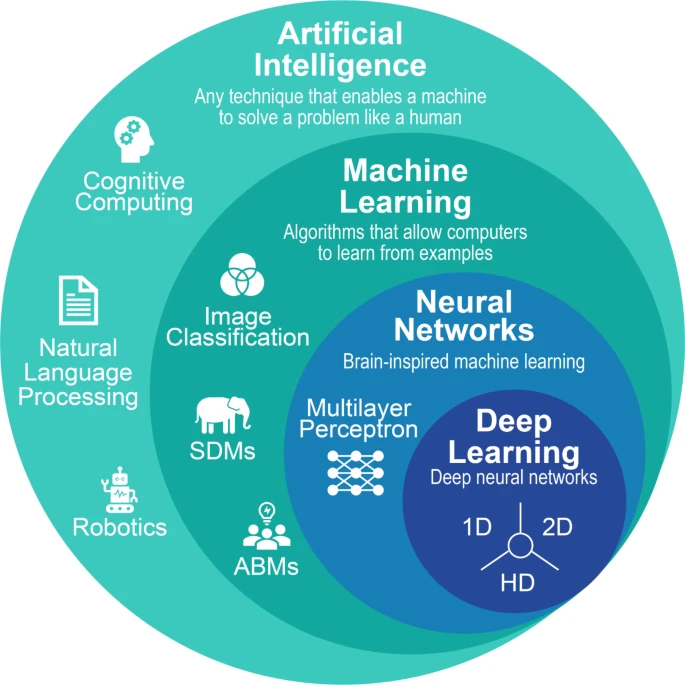
\includegraphics[width=.65\textwidth]{figures/sodoquanhe.png}
\caption[Mối quan hệ giữa AI, học máy, mạng nơ-ron và học sâu]{Mối quan hệ giữa trí tuệ nhân tạo, học máy, mạng nơ-ron và học sâu. }
\label{fig:ai_ml_dl}
\end{figure}

\subsection{Thị giác máy tính và các bài toán cơ bản}
Thị giác máy tính (Computer Vision) khai thác thông tin từ ảnh và video. Xử lý ảnh thường tạo ra một ảnh mới, chẳng hạn ảnh giảm nhiễu hoặc ảnh rõ tương phản hơn; thị giác máy tính dùng những thông tin đó để mô tả đối tượng và cảnh~\cite{tailieu_bai1}. Một hệ thống thị giác có thể sử dụng cả quy tắc xử lý ảnh, mô hình học máy và mạng sâu.

Các nhiệm vụ cơ bản gồm phân loại, phát hiện, phân đoạn và theo dõi. Phân loại trả lời đối tượng thuộc loại nào. Phát hiện còn xác định vị trí bằng khung bao. Phân đoạn xác định các điểm ảnh thuộc từng vùng. Theo dõi liên kết đối tượng qua nhiều khung hình~\cite{szeliski2022vision}. Với ảnh biển báo đã cắt sẵn, hệ thống chỉ cần phân loại vùng ảnh đó; với ảnh đường phố, hệ thống phải tìm biển giữa nhiều vật thể khác trước khi xác định lớp. Nhận dạng ký tự bổ sung bước chuyển chữ và số trong vùng biển thành văn bản.

\subsection{Quá trình thu nhận ảnh}
Ảnh số được tạo từ ánh sáng phản xạ trên vật thể đi qua hệ quang học và tới cảm biến. Lấy mẫu chia mặt phẳng ảnh thành các vị trí rời rạc; lượng tử hoá biểu diễn mức sáng tại mỗi vị trí bằng một tập giá trị hữu hạn. Đây là hai bước khác nhau: tăng số điểm ảnh làm lưới lấy mẫu dày hơn, còn tăng số bit làm các mức cường độ được biểu diễn chi tiết hơn~\cite{tailieu_bai1}.

Diện mạo của một vật trên ảnh phụ thuộc cả đặc điểm bề mặt lẫn nguồn sáng và cách ghi hình. Cùng một mặt biển màu đỏ có thể xuất hiện tối hơn trong bóng râm hoặc nhạt màu khi bị phản sáng. Khi vùng ảnh đã bão hoà trắng hoặc mất chi tiết trong vùng tối, thao tác tăng sáng sau đó không thể tạo lại những nét chưa được ghi nhận.

Chuyển động trong thời gian phơi sáng tạo vệt mờ, còn lấy nét không đúng làm các ranh giới bị trải rộng. Nén ảnh cũng có thể sinh các khối hoặc dao động quanh biên. Vì vậy, độ phân giải không phải tiêu chí duy nhất về chất lượng: một ảnh lớn nhưng mờ có thể chứa ít thông tin nhận dạng hơn một vùng ảnh nhỏ được lấy nét tốt.

\section{Học máy}
\subsection{Các hình thức học và quy trình xây dựng mô hình}
Các hình thức học được phân biệt theo thông tin dùng trong quá trình huấn luyện. Với học có giám sát, mỗi mẫu có nhãn đích, ví dụ ảnh và tên loại biển. Học không giám sát tìm cấu trúc trong dữ liệu chưa có nhãn, như nhóm các ảnh có đặc điểm gần nhau. Học bán giám sát kết hợp cả hai nguồn dữ liệu; một cách thực hiện là chọn các dự đoán đủ tin cậy làm nhãn giả để tiếp tục huấn luyện. Học tăng cường học cách hành động thông qua tương tác với môi trường và phần thưởng~\cite{google_intro_ml,google_ml_types}.

Bảng~\ref{tab:hinhthuchoc} và Hình~\ref{fig:machine_learning} tóm tắt bốn hình thức trên. Việc chọn hình thức học phụ thuộc nhiệm vụ và dữ liệu có sẵn. Phân loại biển từ ảnh có nhãn thường là bài toán có giám sát; phân cụm ảnh phục vụ kiểm tra dữ liệu là ví dụ của học không giám sát.

Một quy trình học máy bắt đầu từ xác định đầu vào và nhãn, kiểm tra dữ liệu, chọn biểu diễn, huấn luyện rồi đánh giá trên các mẫu độc lập. Chất lượng nhãn và cách chia dữ liệu ảnh hưởng trực tiếp đến độ tin cậy của kết quả, ngay cả khi thuật toán được giữ nguyên.

\begin{table}[H]
\centering
\caption[Các hình thức học máy cơ bản]{Các hình thức học máy cơ bản; tổng hợp theo~\cite{google_intro_ml,google_ml_types}.}
\label{tab:hinhthuchoc}
\small
\begin{tabularx}{\textwidth}{|>{\raggedright\arraybackslash}p{2.5cm}|>{\raggedright\arraybackslash}X|>{\raggedright\arraybackslash}X|}
\toprule
\textbf{Hình thức học} & \textbf{Dữ liệu và cách học} & \textbf{Kết quả và ví dụ dễ hình dung} \\
\midrule
Học có giám sát & Dữ liệu có nhãn đúng. Mô hình so sánh dự đoán với nhãn để điều chỉnh tham số. & Dự đoán lớp hoặc giá trị: học từ ảnh đã ghi nhãn để phân loại biển cấm, biển nguy hiểm. \\ \hline
Học không giám sát & Dữ liệu không có nhãn. Mô hình tìm cấu trúc, sự tương đồng hoặc cách biểu diễn gọn hơn. & Phân cụm hoặc giảm chiều: nhóm ảnh biển báo có đặc điểm tương tự để hỗ trợ khám phá dữ liệu. \\ \hline
Học bán giám sát & Kết hợp dữ liệu có nhãn với dữ liệu chưa gán nhãn; có thể dùng nhãn giả được chọn lọc. & Tận dụng ảnh chưa gán nhãn để hỗ trợ huấn luyện; cần kiểm soát nhãn giả sai. \\ \hline
Học tăng cường & Tác nhân thực hiện hành động, nhận thưởng hoặc phạt từ môi trường và học qua tương tác. & Học chính sách tối đa hoá tổng phần thưởng, ví dụ điều khiển xe trong mô phỏng. \\
\bottomrule
\end{tabularx}
\end{table}


\begin{figure}[H]
\centering
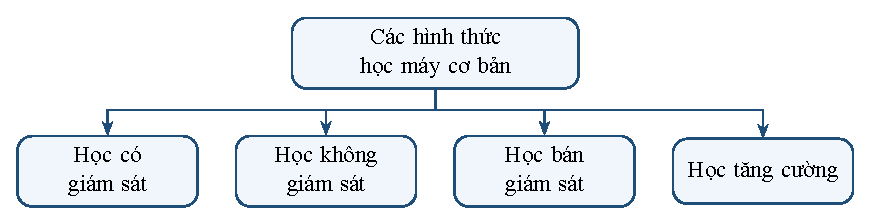
\includegraphics[width=.9\textwidth]{figures/fig_1_2_learning_methods.pdf}
\caption[Các hình thức học máy cơ bản]{Các hình thức học máy cơ bản}
\label{fig:machine_learning}
\end{figure}

\subsection{Các mô hình học máy}
Các mô hình học máy thường nhận một vector đặc trưng và trả về lớp hoặc điểm dự đoán. Màu sắc, hình dạng và cấu trúc nét là những nguồn thông tin có thể đưa vào vector; cách biểu diễn và giảm chiều được trình bày tại Mục~\ref{sec:image_features}.

Máy vector hỗ trợ (Support Vector Machine -- SVM) học ranh giới phân chia các nhóm mẫu với biên phân cách lớn. Các mẫu gần ranh giới có vai trò quyết định cách đặt biên; hàm kernel cho phép xây dựng ranh giới phi tuyến~\cite{cortes1995svm,sklearn_svm}. Với một số mẫu khó, mô hình có thể chấp nhận sai số để cân bằng giữa biên phân cách rộng và mức khớp dữ liệu. Một đặc trưng có giá trị lớn chỉ vì đơn vị đo cũng có thể chi phối khoảng cách, nên cần xem xét chuẩn hoá đầu vào.

Cây quyết định tách dữ liệu bằng những câu hỏi theo đặc trưng, ví dụ tỉ lệ màu có vượt một ngưỡng hay không. Một cây sâu có thể mô tả nhiều trường hợp riêng nhưng dễ phụ thuộc nhiễu. Rừng ngẫu nhiên (Random Forest) tổng hợp dự đoán của nhiều cây được học với sự ngẫu nhiên trong lựa chọn mẫu và đặc trưng. Nhờ đó, kết quả ít phụ thuộc vào một cây đơn lẻ~\cite{sklearn_ensemble}.

LightGBM thuộc nhóm tăng cường cây: các cây được bổ sung theo từng bước để giảm sai số còn lại. Khác với việc tổng hợp nhiều cây học tương đối độc lập, cây mới trong quá trình tăng cường được xây dựng dựa trên thông tin của mô hình hiện tại. Cơ chế chia các giá trị thành những khoảng rời rạc giúp tìm phép tách hiệu quả hơn về thời gian và bộ nhớ~\cite{ke2017lightgbm,lightgbm_features}. Số cây, số lá và tốc độ học ảnh hưởng đến độ phức tạp; tăng các giá trị này không tự bảo đảm dự đoán tốt hơn trên ảnh mới.

Đầu ra của bộ phân loại có thể là nhãn, điểm quyết định hoặc một giá trị biểu diễn mức tin cậy. Các giá trị cùng nằm trong khoảng từ 0 đến 1 chưa chắc đã có cùng ý nghĩa xác suất. Chẳng hạn, trong nhóm mẫu được gán điểm gần $0{,}8$ cho một sự kiện, tỉ lệ sự kiện đó thực sự xảy ra có thể thấp hơn mức này. Hiệu chỉnh điểm dự đoán dùng dữ liệu thích hợp để kiểm tra và điều chỉnh quan hệ đó; nó khác với việc chỉ chọn một ngưỡng chấp nhận~\cite{sklearn_calibration}.

\subsection{Chia dữ liệu, quá khớp và khả năng tổng quát hoá}
Tập huấn luyện được dùng để học tham số. Tập xác thực dùng để lựa chọn mô hình, siêu tham số và ngưỡng quyết định. Tập kiểm thử dùng để đánh giá sau khi các lựa chọn đã được chốt. Những bước học từ dữ liệu như chuẩn hoá hoặc PCA chỉ được khớp trên phần huấn luyện thích hợp, sau đó mới áp dụng sang các tập còn lại~\cite{sklearn_pitfalls}.

Quá khớp xảy ra khi mô hình học quá sát các chi tiết riêng của tập huấn luyện và dự đoán kém trên mẫu mới. Một dấu hiệu thường gặp là sai số huấn luyện tiếp tục giảm nhưng chất lượng xác thực giảm hoặc không cải thiện. Giới hạn độ phức tạp, tăng cường dữ liệu phù hợp và dừng sớm có thể giảm hiện tượng này. Nếu chất lượng trên cả hai tập đều thấp, cần xem lại khả năng biểu diễn, dữ liệu và quá trình huấn luyện.

Ảnh lấy từ cùng một đoạn video có thể gần như trùng nhau. Chia ngẫu nhiên từng ảnh dễ đưa các cảnh rất giống nhau vào cả tập học và tập kiểm thử. Chia theo video, phiên ghi hình hoặc cụm ảnh gần trùng sẽ hạn chế nguy cơ này. Với hệ thống có nhiều mô hình, dữ liệu dùng để huấn luyện bất kỳ thành phần nào đều phải tách khỏi tập kiểm thử của toàn hệ thống.

\section{Mạng nơ-ron và học sâu}
\subsection{Mạng nơ-ron nhân tạo và mạng tích chập}
Một nơ-ron nhân tạo nhận các giá trị đầu vào, tính tổng có trọng số, cộng độ lệch rồi đưa qua hàm kích hoạt. Với đầu vào $\mathbf{x}$, trọng số $\mathbf{w}$ và độ lệch $b$, đầu ra là:
\begin{equation}
 y=\phi(\mathbf{w}^{\top}\mathbf{x}+b).
 \label{eq:neuron}
\end{equation}
Hàm $\phi$ tạo tính phi tuyến; ví dụ ReLU có dạng $\phi(z)=\max(0,z)$. Nhiều lớp nơ-ron kết hợp các biểu diễn trung gian để mô tả quan hệ phức tạp hơn giữa đầu vào và đầu ra~\cite{stanford_neuralnets}.

Mạng nơ-ron tích chập (Convolutional Neural Network -- CNN) xử lý ảnh bằng các bộ lọc nhỏ dùng chung trọng số tại nhiều vị trí. Một bộ lọc có thể phản ứng với nét ngang, nét dọc hoặc một mẫu cục bộ. Với đầu vào một kênh $X$, bộ lọc $K$ kích thước $k\times k$, bước trượt bằng 1 và bỏ qua xử lý biên, ta có:
\begin{equation}
 Y(i,j)=\phi\!\left(b+\sum_{u=0}^{k-1}\sum_{v=0}^{k-1}K(u,v)X(i+u,j+v)\right).
 \label{eq:conv}
\end{equation}
Trong đó $Y(i,j)$ là giá trị đầu ra tại vị trí $(i,j)$; $u,v$ là chỉ số trong bộ lọc. Với đầu vào nhiều kênh, phép tính còn cộng theo các kênh đó. Trong các thư viện học sâu, thao tác này thường gọi là tích chập dù được thực hiện theo dạng tương quan chéo.

Các lớp đầu học những mẫu cục bộ; các lớp sau kết hợp chúng thành biểu diễn rộng hơn. Bước trượt và phần đệm điều chỉnh kích thước bản đồ đặc trưng. Lớp gộp làm giảm độ phân giải, giúp giảm tính toán nhưng cũng có thể làm mất chi tiết của đối tượng nhỏ~\cite{stanford_cs231n_cnn}. Hình~\ref{fig:cnn} minh hoạ một mạng phân loại gồm phần trích đặc trưng và phần đưa ra lớp dự đoán; những kiến trúc khác có thể thay đổi cách tổ chức đầu ra.

Vùng tiếp nhận của một giá trị đặc trưng là phần ảnh đầu vào có thể ảnh hưởng đến nó. Khi đi qua nhiều lớp tích chập và giảm kích thước, vùng tiếp nhận thường mở rộng. Nhờ vậy, các lớp sâu có thể kết hợp nét cục bộ với hình dạng rộng hơn. Tuy nhiên, vùng tiếp nhận lớn không bảo đảm giữ được chi tiết nhỏ nếu chi tiết đã mất trong các bước giảm độ phân giải.

Việc dùng chung bộ lọc giúp CNN nhận ra một mẫu tại nhiều vị trí mà không cần học một bộ trọng số riêng cho từng điểm ảnh. Khả năng này khác với bất biến hoàn toàn trước mọi phép biến đổi. Đổi tỉ lệ, xoay mạnh, thay ánh sáng hoặc che khuất vẫn có thể làm biểu diễn và dự đoán thay đổi. Dữ liệu huấn luyện cần phản ánh những biến đổi có ý nghĩa đối với nhiệm vụ~\cite{stanford_cs231n_cnn}.

Các đầu ra phân loại thường tổng hợp đặc trưng của toàn vùng ảnh. Đầu ra phát hiện còn cần giữ thông tin về vị trí. Do đó, một vector đặc trưng dùng để phân loại ảnh đã cắt không thể được hiểu như danh sách vị trí đối tượng trên cả ảnh; hai kiểu đầu ra đòi hỏi cách tổ chức phần dự đoán khác nhau.

\begin{figure}[H]
\centering
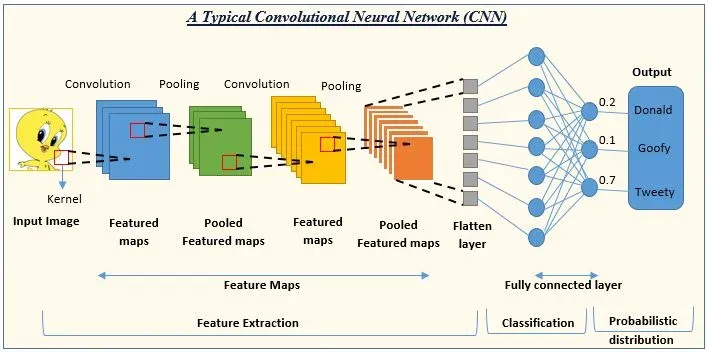
\includegraphics[width=.9\textwidth]{figures/Thuat-toan-CNN-co-cau-truc-nhu-the-nao.png}
\caption[Kiến trúc CNN cơ bản]{Mạng Neural tích chập(CNN) điển hình. nguồn ảnh: InterData~\cite{interdata_cnn_image}.}
\label{fig:cnn}
\end{figure}

\begin{table}[H]
\centering
\caption[So sánh học máy truyền thống và học sâu]{So sánh học máy truyền thống và học sâu trong xử lý ảnh.}
\label{tab:mldl}
\small
\begin{tabularx}{\textwidth}{|>{\raggedright\arraybackslash}p{2.5cm}|>{\raggedright\arraybackslash}X|>{\raggedright\arraybackslash}X|}
\toprule
\textbf{Tiêu chí} & \textbf{Học máy truyền thống} & \textbf{Học sâu} \\
\midrule
Luồng xử lý ảnh & Trích màu, biên, hình dạng hoặc HOG trước; đưa vector đặc trưng vào bộ phân loại. & Mạng nhiều lớp tự học đặc trưng và ánh xạ từ ảnh đến kết quả dự đoán. \\ \hline
Mô hình tiêu biểu & SVM, Random Forest, LightGBM. & CNN; mạng phát hiện đối tượng như YOLO. \\ \hline
Dữ liệu huấn luyện & Thường phù hợp với dữ liệu vừa hoặc nhỏ nếu đặc trưng được chọn tốt. & Huấn luyện từ đầu thường cần nhiều dữ liệu; học chuyển giao giúp giảm nhu cầu này. \\ \hline
Tài nguyên tính toán & Thường nhẹ hơn với vector đặc trưng gọn; nhiều mô hình huấn luyện được trên CPU. & Huấn luyện thường cần GPU; chi phí suy luận phụ thuộc kiến trúc và kích thước ảnh. \\ \hline
Ưu điểm và hạn chế & Dễ kiểm tra đặc trưng; hiệu quả phụ thuộc bước trích chọn, khó bao quát cảnh phức tạp. & Học được đặc trưng phức tạp; cần kiểm soát quá khớp và khó giải thích hơn. \\ \hline
Ví dụ ứng dụng & Kiểm tra vùng nghi ngờ bằng màu, hình dạng và các đặc trưng đã trích xuất. & Phát hiện, phân loại biển báo hoặc nhận dạng chữ trong vùng ảnh. \\
\bottomrule
\end{tabularx}
\end{table}


\subsection{Nguyên lý học của mạng nơ-ron}
Huấn luyện điều chỉnh tham số để giảm hàm mất mát, tức đại lượng đo sai khác giữa dự đoán và nhãn. Lan truyền ngược tính gradient của mất mát theo tham số; thuật toán tối ưu dùng thông tin đó để cập nhật mô hình. Dạng cập nhật cơ bản trên một lô nhỏ dữ liệu là:
\begin{equation}
 \theta_{t+1}=\theta_t-\eta\nabla_{\theta}\mathcal{L}_{\mathcal{B}_t}(\theta_t),
 \label{eq:gradient_update}
\end{equation}
với $\theta_t$ là tham số ở bước $t$, $\eta$ là tốc độ học và $\mathcal{L}_{\mathcal{B}_t}$ là mất mát trên lô $\mathcal{B}_t$. Một lượt đi qua toàn bộ tập huấn luyện được gọi là một epoch. Tốc độ học quá lớn có thể làm quá trình học dao động; tốc độ quá nhỏ làm cập nhật chậm~\cite{goodfellow_optimization}.

Học chuyển giao sử dụng biểu diễn đã học trên dữ liệu nguồn cho một nhiệm vụ mới. Có thể giữ cố định bộ trích đặc trưng và chỉ học phần dự đoán mới, hoặc tiếp tục cập nhật một phần hay toàn bộ mạng. Cách tiếp tục cập nhật này gọi là tinh chỉnh mô hình, hay fine-tuning~\cite{stanford_transfer}.

Với dữ liệu ảnh hạn chế, mô hình huấn luyện trước cung cấp các đặc trưng khởi đầu về biên, màu và kết cấu. Dữ liệu đích vẫn cần đủ đại diện cho điều kiện sử dụng, vì trọng số huấn luyện trước không thay thế được những ví dụ về biển nhỏ, ảnh mờ hoặc ban đêm. Bảng~\ref{tab:mldl} so sánh cách học từ đặc trưng thiết kế trước với cách học biểu diễn bằng mạng sâu.

Trong một lần học có giám sát, hàm mất mát đo sai khác giữa dự đoán và nhãn trên tập mẫu. Với phân loại, sai khác liên quan đến lớp dự đoán; với xác định vị trí, sai khác còn liên quan đến khung bao. Lựa chọn hàm mất mát phải phù hợp đầu ra cần học, trong khi chỉ số đánh giá phản ánh chất lượng theo tiêu chí sử dụng. Mất mát giảm không có nghĩa mọi nhóm lỗi đều giảm như nhau.

Các biện pháp giảm quá khớp có thể tác động vào dữ liệu hoặc mô hình. Tăng cường dữ liệu tạo thêm các biến đổi vẫn giữ được nhãn; giới hạn trọng số hoặc độ phức tạp hạn chế mô hình học những trường hợp quá riêng; dừng sớm chọn thời điểm trước khi chất lượng xác thực suy giảm. Một phép biến đổi làm đổi ý nghĩa đối tượng không còn là tăng cường giữ nguyên nhãn. Ví dụ, lật ngang một ký hiệu có hướng có thể tạo ra một lớp khác.

Khi học chuyển giao, mức khác biệt giữa dữ liệu nguồn và dữ liệu đích ảnh hưởng đến phần mạng nên được điều chỉnh. Giữ cố định nhiều lớp giảm số tham số cần học nhưng cũng hạn chế thích nghi. Cập nhật toàn bộ mạng cho phép thích nghi rộng hơn, đổi lại cần kiểm soát tốc độ học và mức quá khớp. Việc lựa chọn cần dựa trên dữ liệu xác thực, không chỉ dựa vào số lượng lớp của mô hình~\cite{stanford_transfer}.

\subsection{Các phương pháp phát hiện đối tượng}
Phát hiện đối tượng kết hợp phân loại với xác định vị trí. Hai hướng thường gặp là phát hiện hai giai đoạn và một giai đoạn, cũng được giới thiệu trong Bài 9 của tài liệu học phần~\cite{tailieu_bai9}.

Với hướng hai giai đoạn, Faster R-CNN dùng mạng đề xuất vùng để tìm những vị trí có khả năng chứa đối tượng. Đặc trưng ở các vùng này được dùng để phân loại và hiệu chỉnh khung bao. Mạng đề xuất vùng chia sẻ đặc trưng tích chập với mạng phát hiện, giảm việc trích đặc trưng lặp lại~\cite{ren2015faster}.

Với hướng một giai đoạn, các mô hình như YOLO dự đoán khung bao và thông tin lớp trực tiếp từ đặc trưng của ảnh. Cách tổ chức này phù hợp với những ứng dụng cần xử lý liên tiếp nhiều khung hình~\cite{redmon2016yolo,sapkota2025yolo}. Các phiên bản YOLO thay đổi về cấu trúc và cách huấn luyện; cấu trúc lưới của phiên bản đầu không phải mô tả chung cho mọi phiên bản sau.

Kết quả của hai hướng phụ thuộc dữ liệu, kích thước đầu vào, biến thể mạng và phần cứng. Với biển báo nhỏ, việc giảm độ phân giải có thể làm mất những nét giúp phân biệt lớp. Vì vậy cần xem xét đồng thời khả năng định vị, phân loại và thời gian xử lý khi lựa chọn mô hình.

\section{Xử lý ảnh số}
\subsection{Biểu diễn ảnh và các không gian màu}
Ảnh số là một lưới điểm ảnh. Ảnh xám lưu một giá trị cường độ tại mỗi điểm, còn ảnh RGB lưu ba thành phần đỏ, lục và lam. Với ảnh 8 bit mỗi kênh, giá trị thường nằm từ 0 đến 255~\cite{tailieu_bai1}. OpenCV thường đọc ảnh theo thứ tự kênh BGR, nên cần thống nhất thứ tự kênh trước khi hiển thị hoặc đưa ảnh vào mô hình.

HSV mô tả màu bằng sắc màu $H$, độ bão hoà $S$ và độ sáng $V$. Cách tách này thuận tiện để chọn vùng có màu gần nhau. Sắc màu có tính tuần hoàn, vì vậy vùng đỏ có thể nằm ở cả hai đầu miền giá trị $H$. Lab tách độ sáng $L^*$ khỏi hai trục màu: $a^*$ theo hướng lục--đỏ và $b^*$ theo hướng lam--vàng~\cite{opencv_color}. Xử lý riêng độ sáng có thể hạn chế thay đổi màu khi tăng tương phản.

Bảng~\ref{tab:khonggianmau} tóm tắt đặc điểm của từng không gian màu. Trong Hình~\ref{fig:color_spaces}, các kênh được hiển thị riêng bằng thang xám để quan sát giá trị: vùng sáng biểu thị giá trị kênh cao hơn, vùng tối biểu thị giá trị thấp hơn. Đây là cách xem từng kênh, không phải hiện tượng ảnh bị mất màu sau chuyển đổi. Riêng kênh sắc màu, giá trị cao hơn không có nghĩa là màu gốc sáng hơn.

\begin{table}[H]
\centering
\caption{Đặc điểm và vai trò của các không gian màu.}
\label{tab:khonggianmau}
\small
\begin{tabularx}{\textwidth}{|p{2.2cm}|p{3cm}|X|}
\toprule
\textbf{Không gian màu} & \textbf{Các thành phần} & \textbf{Vai trò trong xử lý ảnh} \\
\midrule
RGB & Đỏ, lục, lam & Biểu diễn ảnh màu và hiển thị kết quả \\ \hline
HSV & Sắc màu, độ bão hoà, độ sáng & Tạo mặt nạ vùng màu; phân tích màu đặc trưng của biển \\ \hline
Lab & Độ sáng L và hai thành phần màu a, b & Xử lý độ sáng, tương phản trên kênh L \\
\bottomrule
\end{tabularx}
\end{table}


\begin{figure}[H]
\centering
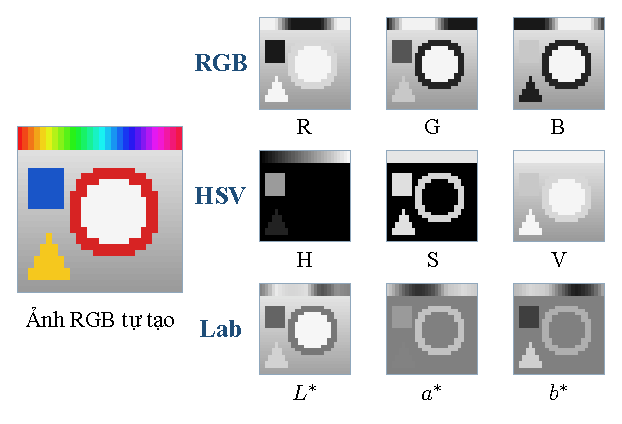
\includegraphics[width=.94\textwidth]{figures/fig_1_4_color_spaces.pdf}
\caption[Minh hoạ các kênh RGB, HSV và Lab]{Minh hoạ các kênh RGB, HSV và Lab . Giá trị các kênh được chuẩn hoá để hiển thị ở thang xám.}
\label{fig:color_spaces}
\end{figure}

\subsection{Lấy mẫu, đổi kích thước và cắt vùng ảnh}
Đổi kích thước ảnh tạo một lưới điểm ảnh mới. Giá trị ở vị trí mới được ước lượng từ các điểm ảnh cũ bằng nội suy. Nội suy láng giềng gần nhất lấy giá trị của điểm gần nhất; nội suy song tuyến tính kết hợp các điểm lân cận; các cách nội suy khác sử dụng vùng rộng hơn hoặc quan hệ diện tích khi thu nhỏ~\cite{opencv_geometry}.

Thu nhỏ làm giảm số điểm biểu diễn đối tượng. Nếu một nét chữ chỉ rộng vài điểm ảnh, nó có thể bị trộn với nền rồi biến mất. Khi phóng to, lưới mới dày hơn nhưng không bổ sung được thông tin chi tiết vốn không có trong ảnh gốc. Vì vậy, kích thước ảnh sau nội suy và lượng thông tin thực còn lại là hai vấn đề cần phân biệt.

Nếu ép một ảnh chữ nhật thành hình vuông bằng hai hệ số co giãn khác nhau, hình tròn có thể thành elip và tỉ lệ nét bị thay đổi. Giữ nguyên tỉ lệ rồi thêm phần đệm tránh biến dạng đó, nhưng phải lưu hệ số tỉ lệ và độ lệch do phần đệm để đổi toạ độ trở lại ảnh ban đầu. Lựa chọn này ảnh hưởng đến cả khung bao và vùng cắt dùng cho các bước sau.

Cắt vùng ảnh giữ lại một phần không gian cần quan sát. Vùng cắt quá hẹp có thể mất viền hoặc ký tự; vùng quá rộng đưa thêm nền và những vật thể khác vào bộ nhận dạng. Với ảnh nhị phân hoặc mặt nạ nhãn, nội suy cũng cần được chọn cẩn thận vì một phép nội suy tạo giá trị trung gian có thể làm thay đổi ý nghĩa của nhãn. Đây là lý do xử lý ảnh màu và xử lý mặt nạ không nhất thiết dùng cùng một phép nội suy.

\subsection{Chất lượng ảnh và điều chỉnh độ sáng}
Độ sáng, tương phản, nhiễu và độ mờ ảnh hưởng đến khả năng quan sát viền và nét chữ. Độ sáng trung bình phản ánh mức sáng chung; độ phân tán cường độ gợi ý mức tương phản. Phương sai đáp ứng Laplacian thường được dùng như một dấu hiệu về độ nét, nhưng nhiễu và nền nhiều chi tiết cũng làm đại lượng này tăng. Các chỉ báo cần được kết hợp và kiểm tra theo loại ảnh sử dụng.

Biến đổi gamma điều chỉnh cường độ để làm sáng hoặc tối ảnh. Cân bằng histogram thích nghi có giới hạn tương phản, thường gọi là CLAHE, thực hiện theo các vùng cục bộ và giới hạn mức tăng tương phản để giảm khuếch đại nhiễu~\cite{zuiderveld1994clahe,opencv_clahe}. Khi thao tác trên kênh độ sáng, màu của ảnh thường ít bị ảnh hưởng hơn so với xử lý độc lập từng kênh RGB.

Histogram là thống kê số điểm ảnh tại từng mức cường độ. Histogram tập trung trong một khoảng hẹp có thể gợi ý tương phản thấp, nhưng không cho biết các điểm sáng và tối nằm ở đâu. Hai ảnh có cách bố trí vật thể khác nhau vẫn có thể có histogram giống nhau. Vì vậy, thống kê toàn ảnh cần được xem cùng cấu trúc cục bộ và nội dung cần nhận dạng.

Với cường độ đã chuẩn hoá $r\in[0,1]$, một cách viết biến đổi gamma là:
\begin{equation}
 s=r^{1/\gamma},\qquad \gamma>0.
 \label{eq:gamma_intensity}
\end{equation}
Trong công thức này, $s$ là đầu ra, $\gamma>1$ làm tăng các mức sáng trung gian và $0<\gamma<1$ làm chúng tối hơn. Cần nêu rõ quy ước vì một số tài liệu viết số mũ trực tiếp là $\gamma$, khi đó chiều tác động của tham số được đảo lại. Hai đầu 0 và 1 vẫn được giữ nguyên.

Cân bằng histogram toàn ảnh dùng một phép biến đổi chung cho mọi vị trí. Với ảnh có vùng sáng và vùng tối khác nhau, tăng tương phản theo vùng có thể phù hợp hơn. CLAHE chia ảnh thành các vùng cục bộ, giới hạn histogram trước khi cân bằng và kết hợp kết quả giữa các vùng để giảm ranh giới giả~\cite{opencv_clahe}. Tăng tương phản cần giữ được các nét thật thay vì chỉ làm mọi chi tiết, kể cả nhiễu, nổi rõ hơn.

\subsection{Lọc nhiễu và làm nổi biên}
Phép lọc xét một vùng lân cận thay vì xử lý độc lập từng điểm ảnh. Lọc trung bình thay một điểm bằng trung bình các điểm quanh nó, nên làm giảm dao động nhưng cũng làm mờ ranh giới. Lọc Gaussian dùng trọng số lớn hơn cho các điểm gần tâm. Khi cửa sổ lọc hoặc độ trải Gaussian tăng, ảnh được làm trơn mạnh hơn và những cấu trúc nhỏ dễ bị mất~\cite{tomasi1998bilateral,opencv_filtering}.

Lọc trung vị sắp các giá trị trong cửa sổ và chọn giá trị ở giữa, phù hợp khi xuất hiện những điểm sáng hoặc tối bất thường rời rạc. Lọc song phương lại xét cả khoảng cách trên ảnh và khác biệt cường độ: hai điểm ở gần nhưng khác màu mạnh có thể được gán mức ảnh hưởng thấp. Nhờ đó một số ranh giới được giữ rõ hơn, nhưng chi phí tính toán và mức lọc vẫn phụ thuộc tham số.

\begin{table}[H]
\centering
\caption{Đặc điểm của một số phép lọc ảnh.}
\label{tab:filters_theory}
\small
\begin{tabularx}{\textwidth}{|>{\raggedright\arraybackslash}p{2.4cm}|>{\raggedright\arraybackslash}X|>{\raggedright\arraybackslash}X|}
\toprule
\textbf{Phép lọc} & \textbf{Cách xử lý} & \textbf{Điểm cần lưu ý} \\
\midrule
Gaussian & Lấy tổng có trọng số theo khoảng cách quanh tâm. & Giảm biến thiên nhỏ nhưng có thể làm mờ biên và nét chữ. \\ \hline
Trung vị & Chọn giá trị giữa trong cửa sổ. & Hữu ích với nhiễu xung; cửa sổ lớn có thể xoá nét mảnh. \\ \hline
Song phương & Kết hợp khoảng cách không gian và khác biệt cường độ. & Có thể giữ biên tốt hơn khi lọc; cần cân nhắc tham số và thời gian. \\
\bottomrule
\end{tabularx}
\end{table}

Đạo hàm ảnh mô tả mức thay đổi cường độ. Với ảnh xám $I$, hai đáp ứng theo chiều ngang và dọc được ký hiệu là $G_x,G_y$. Độ lớn và hướng biến thiên có thể tính bằng:
\begin{equation}
 m=\sqrt{G_x^2+G_y^2},\qquad
 \alpha=\operatorname{atan2}(G_y,G_x).
 \label{eq:gradient_magnitude}
\end{equation}
Độ lớn $m$ phản ánh mức thay đổi tại vị trí xét; góc $\alpha$ chỉ hướng tăng cường độ mạnh nhất, không phải hướng của đường biên. Những toán tử như Sobel ước lượng đạo hàm trên lưới ảnh; Laplacian sử dụng đạo hàm bậc hai để làm nổi những thay đổi cục bộ~\cite{opencv_gradients}.

Biên thật, nhiễu và các vân nền đều có thể tạo đáp ứng đạo hàm lớn. Lọc trước khi tính biên thường giúp giảm ảnh hưởng của nhiễu nhưng có thể làm yếu nét nhỏ. Đáp ứng có dấu cũng cần được lưu bằng kiểu số phù hợp; chuyển ngay sang số nguyên không dấu có thể làm mất phần âm. Kết quả tính biên là thông tin để mô tả hoặc phân vùng, chưa phải kết luận đối tượng thuộc lớp nào.

\subsection{Phân vùng ảnh và đặc trưng hình dạng}
Phân vùng ảnh tách các điểm ảnh thành những vùng có ý nghĩa, chẳng hạn mặt nạ vùng đỏ hoặc vùng sáng chứa chữ. Ngưỡng theo màu là cách thực hiện đơn giản, nhưng nhạy với ánh sáng và bóng đổ. Phát hiện biên tìm nơi cường độ biến đổi mạnh; đường bao mô tả ranh giới của một vùng. Một ảnh biên có thể chứa nhiều đoạn rời, chưa tạo thành đường bao hoàn chỉnh của đối tượng.

Các phép hình thái học dùng phần tử cấu trúc, tức một mẫu lân cận nhỏ, để điều chỉnh hình dạng vùng. Trên ảnh nhị phân có tiền cảnh trắng, phép co làm thu hẹp vùng trắng, phép giãn làm mở rộng vùng trắng. Phép mở là co rồi giãn, thường loại đốm nhỏ; phép đóng là giãn rồi co, có thể lấp lỗ nhỏ hoặc khe hẹp~\cite{opencv_morphology}. Kích thước phần tử cấu trúc cần phù hợp với chi tiết muốn giữ.

Hàng trên của Hình~\ref{fig:morphology_shapes} minh hoạ bốn phép xử lý với cùng một ảnh nhị phân. Hàng dưới là các hình học độc lập để minh hoạ đặc trưng: nét đỏ chỉ đường bao, nét xanh đứt chỉ khung chữ nhật bao quanh, chấm đen chỉ tâm. Hình tròn, tam giác và hình vuông xoay nghiêng không phải kết quả của các phép xử lý ở hàng trên.

Từ đường bao có thể tính diện tích, chu vi, tâm và số đỉnh sau xấp xỉ đa giác~\cite{opencv_contours}. Độ tròn là một ví dụ:
\begin{equation}
 C=\frac{4\pi A}{P^2},
 \label{eq:circularity}
\end{equation}
trong đó $A$ là diện tích, $P$ là chu vi. Hình tròn lý tưởng có $C=1$; những hình kém tròn có giá trị nhỏ hơn. Trên ảnh số, cách lấy đường bao ảnh hưởng đến kết quả. Tỉ lệ rộng/cao, độ đặc (diện tích vùng chia cho diện tích bao lồi) và số đỉnh bổ sung thông tin về hình dạng. Góc nhìn nghiêng có thể làm biển tròn xuất hiện thành elip, nên cần kết hợp các đặc trưng thay vì dùng một ngưỡng loại bỏ cứng.

Số đỉnh của một đường bao được xác định sau khi xấp xỉ thành đa giác. Mức cho phép sai lệch nhỏ giữ nhiều chi tiết, kể cả răng cưa do ảnh số; mức lớn hơn làm đường bao gọn nhưng có thể mất góc thật. Vì vậy, việc đếm ba hay bốn đỉnh phải đi cùng cách xấp xỉ và chất lượng mặt nạ, thay vì xem là tính chất luôn ổn định của vùng ảnh.

Moment mô tả cách các điểm của một vùng phân bố trong mặt phẳng. Với mặt nạ nhị phân $M(x,y)$ nhận giá trị 1 trong vùng và 0 ngoài vùng, moment bậc $(p,q)$ là:
\begin{equation}
 m_{pq}=\sum_x\sum_y x^p y^q M(x,y).
 \label{eq:region_moment}
\end{equation}
Ở đây $p,q$ là các số nguyên không âm. $m_{00}$ đếm diện tích theo điểm ảnh; khi $m_{00}>0$, tâm vùng có toạ độ $m_{10}/m_{00}$ và $m_{01}/m_{00}$. Trừ toạ độ tâm trước khi tính moment giúp loại ảnh hưởng tịnh tiến; bước chuẩn hoá tiếp theo giảm ảnh hưởng của kích thước.

Bảy moment Hu được tạo từ các moment đã chuẩn hoá để mô tả hình dạng với tính bất biến đối với tịnh tiến, thay đổi tỉ lệ và quay trong mô hình lý tưởng~\cite{hu1962moments,opencv_shape_descriptors}. Trên ảnh rời rạc, chúng vẫn thay đổi do nội suy, nhiễu, che khuất và góc nhìn. Các moment vì vậy bổ sung mô tả của toàn vùng, không thay cho đường bao hay ký hiệu bên trong. Với phép phản chiếu, dấu của moment Hu thứ bảy có thể thay đổi.

\begin{figure}[H]
\centering
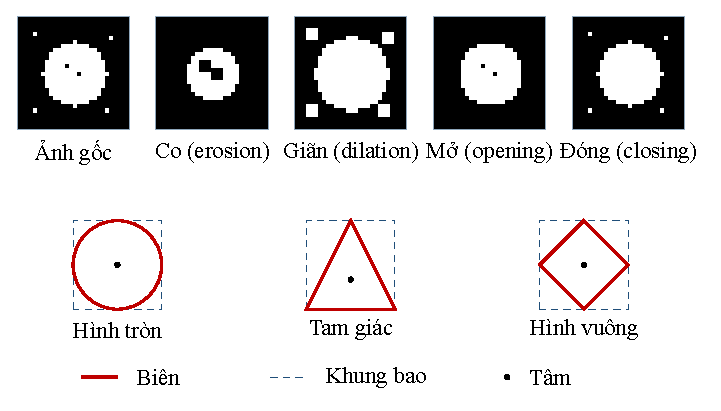
\includegraphics[width=\textwidth]{figures/fig_1_4_morphology_shapes.pdf}
\caption[Phép hình thái học và đặc trưng hình dạng]{Phép co, giãn, mở, đóng trên ảnh nhị phân tự tạo với kernel vuông $3\times3$; bên dưới minh hoạ biên, khung bao và tâm của các hình cơ bản.}
\label{fig:morphology_shapes}
\end{figure}

\subsection{Biến đổi ảnh trong miền tần số}
Trong miền không gian, ảnh được mô tả bằng cường độ tại các vị trí. Trong miền tần số, ảnh được biểu diễn qua các thành phần biến thiên chậm hoặc nhanh. Vùng nền tương đối đồng đều chủ yếu đóng góp vào tần số thấp, còn nét mảnh, đường biên và một phần nhiễu tạo thành phần tần số cao. Bài 2 trình bày hai cách biến đổi thường gặp là Fourier rời rạc và cosin rời rạc~\cite{tailieu_bai2}.

Biến đổi Fourier dùng các thành phần hình sin và cos để mô tả biến thiên theo hai hướng của ảnh. Biên độ thể hiện mức đóng góp của thành phần tần số, còn pha liên quan đến cách các thành phần được sắp xếp trong không gian. Chỉ giữ thông tin biên độ không đủ để tái tạo vị trí chi tiết ban đầu.

Biến đổi cosin rời rạc, thường viết tắt là DCT, biểu diễn ảnh bằng tổng các mẫu cosin. Với nhiều ảnh tự nhiên, phần lớn năng lượng có thể tập trung vào một nhóm hệ số tần số thấp. Điều này cho phép tạo một biểu diễn gọn về cấu trúc tổng thể. Nếu bỏ các hệ số tần số cao, những nét nhỏ cũng có thể bị mất; vì vậy cách rút gọn này không phù hợp để bảo toàn mọi ký tự.

Miền tần số giải thích đánh đổi khi làm trơn: giảm biến thiên nhanh có thể giảm nhiễu nhưng đồng thời làm yếu biên. Tuy nhiên, không thể coi mọi tần số cao là nhiễu và mọi tần số thấp là thông tin cần giữ. Trong so sánh ảnh gần trùng, các thành phần thấp có thể làm dấu hiệu về bố cục chung; trong nhận dạng ký hiệu, chính những nét nhỏ lại có thể quyết định sự khác nhau giữa hai lớp. Cách sử dụng phụ thuộc mục đích của biểu diễn.

\section{Đặc trưng ảnh và giảm chiều dữ liệu}
\label{sec:image_features}
\subsection{Màu sắc, hình dạng và kết cấu}
Đặc trưng chuyển vùng ảnh thành một tập giá trị có cùng quy ước để các mẫu được so sánh hoặc đưa vào mô hình. Đặc trưng màu mô tả phân bố màu; đặc trưng hình dạng mô tả đường bao hay vùng; đặc trưng kết cấu mô tả cách cường độ thay đổi trong một lân cận. Bài 3 phân biệt những thông tin trực tiếp từ điểm ảnh với biểu diễn được tổng hợp trên phạm vi rộng hơn~\cite{tailieu_bai3}.

Tỉ lệ điểm ảnh thuộc một khoảng màu là một đặc trưng đơn giản, ít phụ thuộc kích thước vùng hơn số điểm ảnh tuyệt đối. Tuy nhiên, tỉ lệ đó không cho biết màu nằm ở viền hay ở giữa. Histogram màu cũng bỏ qua nhiều thông tin vị trí. Hai vật thể có cách sắp xếp màu khác nhau vẫn có thể cho biểu diễn gần nhau, nên thường cần thêm thông tin hình dạng hoặc cấu trúc nét.

Đặc trưng cục bộ mô tả một vùng nhỏ quanh điểm nổi bật; đặc trưng toàn vùng tổng hợp cả vùng quan tâm. Các mô tả điểm ở Bài 4 minh hoạ nhu cầu giữ thông tin khi đối tượng thay đổi tỉ lệ hoặc hướng nhìn~\cite{tailieu_bai4}. Lựa chọn giữa hai kiểu mô tả phụ thuộc nhiệm vụ: một vùng rất nhỏ có thể không có đủ điểm nổi bật ổn định, còn một vector toàn vùng lại nhạy với phần nền bị cắt vào.

Khi ghép nhiều loại đặc trưng, cần giữ đúng thứ tự và cách tính ở cả bước học lẫn bước sử dụng. Một giá trị thiếu do không tìm được đường bao phải được phân biệt với giá trị đo bằng 0. Các bước đổi kích thước vùng, chọn mặt nạ và chuẩn hoá cũng là một phần của biểu diễn, vì thay chúng có thể làm vector đầu vào khác với dữ liệu mà mô hình đã học.

\subsection{Mô tả hướng biên}
Bộ mô tả hướng biên HOG thống kê cách các nét phân bố trong vùng ảnh. Thay vì ghi chính xác cường độ của từng điểm, nó gom các hướng biến thiên vào những ô nhỏ. Hai vùng có mức sáng khác nhau nhưng cấu trúc nét gần giống nhau có thể nhận được biểu diễn gần nhau hơn so với việc so trực tiếp từng điểm ảnh~\cite{tailieu_bai5,dalal2005hog}.

Quá trình trích đặc trưng bắt đầu từ một vùng có kích thước thống nhất. Tại mỗi điểm, đạo hàm theo hai hướng được dùng để tính độ lớn và góc theo~\eqref{eq:gradient_magnitude}. Trong mỗi ô, các điểm đóng góp vào histogram hướng, thường có trọng số theo độ lớn. Với biểu diễn không phân biệt dấu, hai hướng chênh $180^\circ$ được gộp lại vì chúng mô tả cùng một phương của nét.

Các ô lân cận được ghép thành khối và chuẩn hoá. Nếu chỉ nhân độ sáng của ảnh với một hệ số, các độ lớn gradient có xu hướng cùng tăng; chuẩn hoá theo khối làm giảm ảnh hưởng của sự thay đổi đó. Các khối có thể chồng lấn để cùng một vị trí được xem trong nhiều lân cận, sau đó các vector khối được nối theo thứ tự cố định~\cite{skimage_hog}.

Có thể hình dung một ví dụ gồm $4\times4$ ô, mỗi ô có 9 khoảng hướng. Nếu mỗi khối gồm $2\times2$ ô và dịch từng ô một, ta có $3\times3$ khối. Mỗi khối có $2\times2\times9=36$ giá trị, nên vector cuối có $3\times3\times36=324$ thành phần. Đây là ví dụ cách xác định số chiều, không phải một kích thước bắt buộc của HOG.

Ô nhỏ mô tả nét chi tiết hơn nhưng nhạy với nhiễu và làm vector dài hơn. Ô lớn tạo biểu diễn gọn hơn nhưng có thể trộn các nét cần phân biệt. HOG cũng không tự bất biến trước mọi phép quay hoặc biến dạng phối cảnh. Chất lượng vùng cắt và lượng chi tiết của ảnh vẫn quyết định thông tin còn lại trong vector.

\subsection{Phân tích thành phần chính}
Phân tích thành phần chính (Principal Component Analysis -- PCA) tìm một hệ trục mới để biểu diễn dữ liệu bằng ít chiều hơn. Những chiều ban đầu có thể chứa thông tin liên quan nhau; giữ tất cả làm tăng bộ nhớ và chi phí tính toán. PCA chọn các hướng có phương sai lớn để giữ phần biến thiên chủ yếu của tập dữ liệu~\cite{tailieu_bai8}.

Giả sử có $n$ vector $\mathbf{x}_i\in\mathbb{R}^{d}$. Trước hết tính vector trung bình $\boldsymbol{\mu}$ và ma trận hiệp phương sai $S$:
\begin{equation}
 \boldsymbol{\mu}=\frac{1}{n}\sum_{i=1}^{n}\mathbf{x}_i,\qquad
 S=\frac{1}{n-1}\sum_{i=1}^{n}(\mathbf{x}_i-\boldsymbol{\mu})(\mathbf{x}_i-\boldsymbol{\mu})^{\top},
 \label{eq:pca_covariance}
\end{equation}
với $n>1$. Các vector riêng trực chuẩn của $S$ xác định những hướng mới; trị riêng cho biết phương sai theo từng hướng. Sau khi sắp theo trị riêng giảm dần, chọn $r<d$ hướng đầu thành các cột của ma trận $U_r\in\mathbb{R}^{d\times r}$. Vector trong không gian giảm chiều là:
\begin{equation}
 \mathbf{z}_i=U_r^{\top}(\mathbf{x}_i-\boldsymbol{\mu}).
 \label{eq:pca_projection}
\end{equation}
Như vậy, $d$ giá trị ban đầu được thay bằng $r$ toạ độ mới; đây là tổ hợp của các đặc trưng cũ, không đơn thuần là xoá một số vị trí trong vector.

Số chiều giữ lại có thể được chọn theo tỉ lệ tổng phương sai hoặc kiểm tra theo nhiệm vụ sử dụng. Giữ nhiều chiều bảo toàn thêm biến thiên nhưng giảm ít chi phí. Giữ quá ít có thể làm mất những nét phân biệt quan trọng. PCA không dùng nhãn lớp để chọn hướng, nên phương sai lớn không đồng nghĩa với khả năng phân loại tốt.

PCA cần trừ trung bình; việc có chuẩn hoá từng đặc trưng về cùng thang đo trước đó hay không là một lựa chọn riêng. Ví dụ, ghép chu vi tính bằng điểm ảnh với tỉ lệ màu trong khoảng 0 đến 1 có thể khiến nhóm giá trị lớn ảnh hưởng mạnh hơn nếu không xử lý thang đo. Tài liệu scikit-learn cũng phân biệt việc trừ trung bình với việc chia theo độ lệch chuẩn~\cite{sklearn_pca}.

Vector trung bình, phép chuẩn hoá và các trục PCA phải được học trên phần huấn luyện thích hợp rồi giữ cố định khi biến đổi dữ liệu xác thực, kiểm thử hoặc ảnh mới. Nếu tính lại trên toàn bộ dữ liệu trước khi chia, thông tin của tập kiểm thử đã ảnh hưởng tới biểu diễn. Cùng một bộ trích đặc trưng nhưng khác bộ PCA cũng tạo ra không gian đầu vào khác nhau.

\subsection{Độ tương đồng và ảnh gần trùng}
So sánh ảnh thường được thực hiện thông qua biểu diễn của chúng. Bài 6 giới thiệu việc dùng khoảng cách giữa các vector để tìm những mô tả gần nhau~\cite{tailieu_bai6}. Khoảng cách nhỏ chỉ có ý nghĩa trong quy ước đặc trưng đã chọn: gần nhau về màu không nhất thiết là cùng đối tượng, còn gần nhau về hình dạng chưa chắc có cùng nội dung chữ.

Hai tệp có thể khác dữ liệu lưu nhưng vẫn cho những ảnh nhìn gần giống nhau, chẳng hạn một ảnh được nén lại hoặc đổi kích thước. Ngược lại, hai ảnh khác cảnh có thể cùng chứa một loại biển. Cần phân biệt trùng tệp, gần trùng về nội dung ảnh và giống nhau về lớp đối tượng, vì chúng phục vụ các mục đích kiểm tra khác nhau.

Mã băm cảm nhận tạo một chuỗi bit ngắn mô tả những dấu hiệu tổng thể của ảnh. Một cách tạo mã là chuyển ảnh về xám, đổi về kích thước thống nhất, tính DCT, lấy một vùng hệ số tần số thấp rồi so với giá trị trung vị để tạo bit~\cite{imagehash_phash}. Đây là ứng dụng của biểu diễn tần số để so sánh bố cục, không phải mã hoá bảo mật hoặc phương pháp đọc nội dung biển.

Với hai mã $h^{(1)},h^{(2)}$ cùng có $L$ bit, khoảng cách Hamming là số vị trí khác nhau:
\begin{equation}
 d_H(h^{(1)},h^{(2)})=\sum_{j=1}^{L}\mathbf{1}[h_j^{(1)}\ne h_j^{(2)}].
 \label{eq:hamming_hash}
\end{equation}
Ký hiệu $\mathbf{1}$ bằng 1 khi điều kiện đúng và bằng 0 khi sai. Khoảng cách nhỏ gợi ý hai biểu diễn giống nhau hơn. Ngưỡng quá rộng có thể gộp nhầm những cảnh khác; ngưỡng quá chặt có thể bỏ qua các bản gần trùng. Ảnh bị cắt nhiều, quay mạnh hoặc có bố cục thay đổi cũng có thể cho mã khác dù cùng nguồn.

Kiểm tra gần trùng giúp hạn chế thông tin lặp giữa các tập dữ liệu. Các nhóm nghi ngờ cần được duyệt cùng nguồn ghi hình trước khi chia tập. Trong một cụm ghép nối tiếp, hai ảnh ở hai đầu vẫn có thể khác nhau đáng kể.


% ==============================================================================
\section{Các nghiên cứu liên quan}
\label{sec:related_work}

Mục này tổng hợp các công trình về nhận diện biển báo theo bốn nhóm: bộ dữ liệu và cách đánh giá, phương pháp truyền thống, phương pháp học sâu cho biển nhỏ, theo vết và xác minh trên video. Mọi tài liệu đã được đối chiếu với nơi công bố (DOI hoặc trang của nhà xuất bản). Số liệu của các công trình khác dùng tập dữ liệu, cách chia và chỉ số khác với đề tài, nên chỉ dùng làm bối cảnh, không so sánh trực tiếp.

\subsection{Bộ dữ liệu và cách đánh giá}
\label{sec:rw_data}

Hai bộ dữ liệu của Đức tách bài toán thành hai phần. GTSRB là bài toán phân loại vùng biển đã cắt sẵn với 43 lớp; trong cuộc thi, một tổ hợp mạng tích chập đạt tỉ lệ phân loại đúng cao hơn người tham gia thử nghiệm~\cite{stallkamp2012gtsrb}. GTSDB là bài toán phát hiện trên ảnh đường phố (900 ảnh, 600 để huấn luyện và 300 để đánh giá), đánh giá riêng theo nhóm biển cấm, nguy hiểm và hiệu lệnh~\cite{houben2013gtsdb}. Việc tách hai phần cho thấy độ chính xác phân loại trên vùng đã cắt không thay thế được chỉ số phát hiện trên cả ảnh. Đề tài áp dụng nguyên tắc này khi so sánh phương pháp truyền thống với YOLO (Mục~\ref{sec:e8}).

Tsinghua-Tencent 100K (TT100K) có 100 nghìn ảnh toàn cảnh với khoảng 30 nghìn biển, phần lớn chiếm diện tích rất nhỏ trong ảnh. Các tác giả chỉ ra rằng mạng phát hiện thiết kế cho vật thể lớn hoạt động kém với biển nhỏ~\cite{zhu2016tt100k}. Bộ dữ liệu Mapillary mở rộng phạm vi ra toàn cầu, có lớp \textit{other-sign} cho biển nằm ngoài danh mục và báo cáo kết quả theo kích thước biển~\cite{ertler2020mapillary}. Đây là tiền lệ cho lớp ``Biển báo khác'' và cho cách phân tích theo kích thước của đề tài.

Với biển báo Việt Nam, Zalo AI Challenge 2020 cung cấp ảnh đường phố độ phân giải $1622\times626$ có nhiều biển rất nhỏ~\cite{zalo2020tsd}; ảnh cùng độ phân giải này chiếm 41\% bộ dữ liệu của đề tài. Pham và cộng sự xây dựng mô-đun nhận diện dựa trên YOLOv5, huấn luyện trên dữ liệu tự thu ngoài đường và chạy trên thiết bị Jetson~\cite{tung2024vietnam}. Cu và cộng sự xây dựng bộ dữ liệu biển nguy hiểm và cảnh báo theo QCVN~41:2019 và dùng YOLOv5 để phát hiện~\cite{cu2024vietnamese,qcvn41_2019}. Các công trình này dùng bộ dữ liệu riêng và chưa so sánh với phương pháp truyền thống trên cùng tập kiểm thử.

\subsection{Phương pháp thị giác máy tính truyền thống}
\label{sec:rw_classic}

Hướng kinh điển gồm hai bước: tìm vùng ứng viên theo màu và hình dạng, sau đó nhận dạng vùng đó. De la Escalera và cộng sự định vị biển bằng ngưỡng màu và hình dạng rồi nhận dạng bằng mạng nơ-ron~\cite{escalera1997road}. Maldonado-Bascón và cộng sự dùng ba giai đoạn: phân đoạn màu, phân loại hình dạng bằng SVM tuyến tính và nhận dạng nội dung bằng SVM nhân Gauss~\cite{maldonado2007svm}. Ưu điểm của hướng này là nhanh và dễ giải thích; nhược điểm là ngưỡng màu thay đổi theo ánh sáng và hình dạng bị biến dạng theo góc nhìn.

HOG mô tả hình dạng bằng histogram hướng gradient trên lưới ô và chuẩn hoá theo khối~\cite{dalal2005hog}. Trên GTSDB, HOG kết hợp bộ phân loại tuyến tính là một trong các phương pháp cơ sở~\cite{houben2013gtsdb}. Vieira so sánh các bước tiền xử lý cho HOG-SVM trên GTSRB: độ chính xác tăng từ 89,65\% lên 91,25\% khi chuyển sang không gian YUV, còn ghép nhiều bước (CLAHE, kênh Hue, YUV) không phải lúc nào cũng tốt hơn~\cite{vieira2025hogsvm}. Đặc trưng điểm khoá như SIFT~\cite{lowe2004sift} kết hợp túi từ thị giác~\cite{csurka2004bovw} hiệu quả với vật thể giàu kết cấu; biển báo lại có ít điểm đặc trưng, nhất là khi biển nhỏ. Đề tài dùng SIFT làm đối chứng âm để kiểm chứng nhận định này (Mục~\ref{sec:e8}).

\subsection{Học sâu và vấn đề biển nhỏ}
\label{sec:rw_deep}

Bộ phát hiện hai giai đoạn như Faster R-CNN đề xuất vùng rồi phân loại~\cite{ren2015faster}; họ YOLO dự đoán khung và lớp trong một lần truyền, phù hợp xử lý thời gian thực~\cite{redmon2016yolo}. Bài tổng quan của Sapkota và cộng sự hệ thống hoá các phiên bản từ YOLOv1 đến YOLOv12~\cite{sapkota2025yolo}. YOLO11 thay đổi khối trích đặc trưng (C3k2, C2PSA) và có nhiều kích cỡ từ \textit{nano} đến \textit{extra-large}~\cite{khanam2024yolo11,ultralytics_yolo11}. Các mô hình này thường được khởi tạo từ trọng số học trên COCO~\cite{lin2014coco} rồi tinh chỉnh cho bài toán đích.

Biển nhỏ là thách thức chung. Với ảnh độ phân giải cao, SAHI chia ảnh thành các ô chồng lấn, chạy bộ phát hiện trên từng ô rồi gộp kết quả. Chỉ riêng bước suy luận cắt ô đã tăng AP 5,1--6,8 điểm trên VisDrone và xView; khi tinh chỉnh thêm trên ô cắt, mức tăng lên 12,7--14,5 điểm~\cite{akyon2022sahi}. Lời giải của nhiều đội tại Zalo AI 2020 cũng dùng cắt ô vì biển rất nhỏ~\cite{zalo2020tsd}. Đề tài không thể bổ sung dữ liệu, nên chỉ thử những cách không cần huấn luyện lại: tăng độ phân giải suy luận và cắt ô khi suy luận (Mục~\ref{sec:t3}).

\subsection{Theo vết và xác minh trên video}
\label{sec:rw_video}

SORT kết hợp bộ lọc Kalman~\cite{kalman1960filter} để dự đoán vị trí và thuật toán Hungarian~\cite{kuhn1955hungarian} để ghép phát hiện theo IoU. Phương pháp rất đơn giản nhưng đạt độ chính xác tương đương các bộ theo vết trực tuyến cùng thời và chạy khoảng 260 khung hình mỗi giây; tác giả cũng nhận xét chất lượng theo vết phụ thuộc nhiều vào bộ phát hiện~\cite{bewley2016sort}. Với biển báo, Šegvić và cộng sự xây dựng chuỗi phát hiện nhất quán theo thời gian rồi lọc chuỗi bằng một mô hình phân biệt học riêng~\cite{segvic2014temporal}. Đây là cơ sở cho thiết kế theo vết và bộ xác minh trong hệ thống của nhóm.

\subsection{Tổng hợp và khoảng trống}
\label{sec:rw_gap}

Bảng~\ref{tab:related_work} tóm tắt các công trình chính và vai trò của chúng trong đề tài.

\begin{table}[H]
\centering
\caption{Tóm tắt các nghiên cứu liên quan}
\label{tab:related_work}
\small
\begin{tabularx}{\textwidth}{|>{\raggedright\arraybackslash}p{3.3cm}|>{\centering\arraybackslash}p{1.2cm}|>{\raggedright\arraybackslash}X|>{\raggedright\arraybackslash}p{4.1cm}|}
\toprule
\textbf{Công trình} & \textbf{Năm} & \textbf{Nội dung chính} & \textbf{Vai trò trong đề tài} \\
\midrule
De la Escalera và cs.~\cite{escalera1997road} & 1997 & Định vị theo màu + hình dạng, nhận dạng bằng mạng nơ-ron & Cơ sở của pipeline CV đối chứng \\ \hline
Maldonado-Bascón và cs.~\cite{maldonado2007svm} & 2007 & Phân đoạn màu, SVM cho hình dạng và nội dung & Cơ sở dùng SVM sau ứng viên màu \\ \hline
Dalal, Triggs~\cite{dalal2005hog} & 2005 & Đặc trưng HOG & Đặc trưng thủ công chính \\ \hline
GTSRB, GTSDB~\cite{stallkamp2012gtsrb,houben2013gtsdb} & 2012, 2013 & Tách đánh giá phân loại và phát hiện & Thiết kế thí nghiệm E8 \\ \hline
TT100K~\cite{zhu2016tt100k} & 2016 & Biển nhỏ trong ảnh toàn cảnh & Phân tích theo kích thước \\ \hline
Mapillary~\cite{ertler2020mapillary} & 2020 & Phạm vi toàn cầu, lớp \textit{other-sign} & Lớp ``Biển báo khác'' \\ \hline
SAHI~\cite{akyon2022sahi} & 2022 & Suy luận và tinh chỉnh trên ô cắt & Thí nghiệm T3 \\ \hline
SORT~\cite{bewley2016sort} & 2016 & Kalman + Hungarian theo IoU & Mô-đun theo vết \\ \hline
Šegvić và cs.~\cite{segvic2014temporal} & 2014 & Chuỗi theo vết + bộ lọc phân biệt & Bộ xác minh \\ \hline
Vieira~\cite{vieira2025hogsvm} & 2025 & Tiền xử lý cho HOG-SVM & Mốc tham chiếu HOG-SVM \\ \hline
Pham và cs.~\cite{tung2024vietnam}; Cu và cs.~\cite{cu2024vietnamese} & 2024 & YOLOv5 cho biển báo Việt Nam & Bối cảnh trong nước \\
\bottomrule
\end{tabularx}
\end{table}

Từ tổng hợp trên, đề tài hướng tới ba vấn đề còn ít được xem xét:
\begin{enumerate}
 \item So sánh trực tiếp phương pháp truyền thống và học sâu trên cùng tập kiểm thử biển báo Việt Nam, theo từng nhóm kích thước biển và có khoảng tin cậy.
 \item Đo đóng góp của từng khâu xử lý ảnh truyền thống trong một hệ thống học sâu, gồm cả những khâu không mang lại cải thiện.
 \item Cải thiện recall biển nhỏ và độ bền với ảnh tối khi không thể bổ sung dữ liệu: tăng độ phân giải suy luận, cắt ô và tăng cường ảnh thích nghi.
\end{enumerate}


\chapter{PHƯƠNG PHÁP VÀ MÔ HÌNH}
\label{chap:chuong2}

Chương này trình bày phương pháp của hệ thống nhận diện biển báo giao thông. Hệ thống dùng hai nhóm phương pháp theo yêu cầu của học phần. Nhóm học sâu gồm YOLO11 để phát hiện và phân loại, VietOCR để đọc chữ và số. Nhóm thị giác máy tính truyền thống gồm đánh giá chất lượng ảnh, tăng cường ảnh thích nghi, theo vết bằng bộ lọc Kalman, và một pipeline đối chứng hoàn toàn bằng đặc trưng thủ công (màu, hình dạng, HOG) với SVM. Chương lần lượt trình bày phát biểu bài toán, dữ liệu, kiến trúc tổng thể, từng phương pháp và cách tổ chức huấn luyện, đánh giá. Kết quả thực nghiệm được trình bày ở Chương~\ref{chap:chuong3}.

\section{Phát biểu bài toán nhận diện biển báo}
\label{sec:baitoannhandien}
\subsection{Mô tả bằng lời}
Phát hiện biển báo xác định vị trí của biển trong cảnh bằng khung bao. Phân loại gán tên lớp cho vùng biển đã tìm được. Nhận dạng chữ và số đọc nội dung bên trong vùng ảnh. Hệ thống cần kết hợp ba nhiệm vụ này để trả về thông tin sử dụng được.

Đầu vào là một ảnh màu hoặc một chuỗi khung hình từ video, camera. Trong mỗi ảnh, hệ thống tìm các biển thuộc bộ nhãn đã chọn, xác định vị trí và trả về tên lớp cùng điểm tin cậy. Với biển có chữ hoặc giá trị số, hệ thống đọc thêm nội dung khi vùng ảnh đủ rõ. Với video, các lần quan sát của cùng một biển được gắn cùng mã theo vết để tổng hợp thông tin và hạn chế thông báo lặp.

Ví dụ, khi gặp biển giới hạn tốc độ, đầu ra cần có khung bao, tên lớp và giá trị đọc được, chẳng hạn 40 km/h. Nếu vùng số quá nhỏ, hệ thống vẫn trả kết quả phát hiện và để trống nội dung số. Tên và ý nghĩa hiển thị được tra từ danh mục lớp theo QCVN~41:2019/BGTVT~\cite{qcvn41_2019}, còn giá trị cụ thể phải được đọc từ ảnh. Hình~\ref{fig:traffic_sign_tasks} minh hoạ thông tin nhận diện mong muốn.

\begin{figure}[H]
\centering
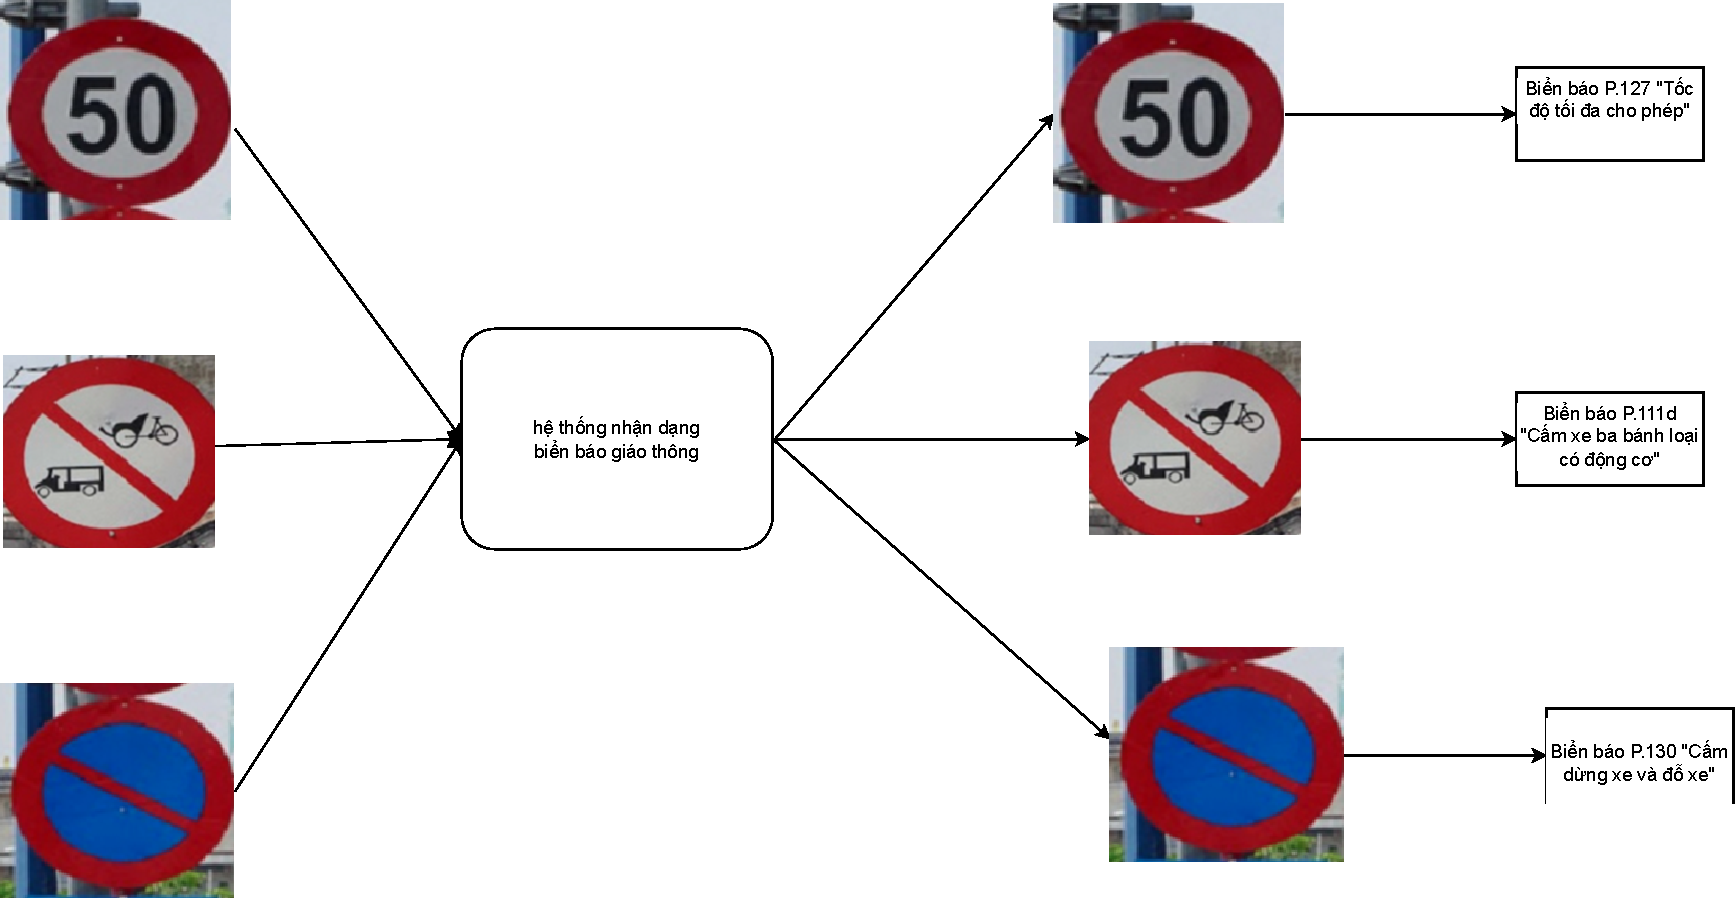
\includegraphics[width=\textwidth]{figures/anhnhandien.pdf}
\caption[Minh hoạ bài toán nhận diện biển báo giao thông]{Minh hoạ bài toán nhận diện biển báo giao thông}
\label{fig:traffic_sign_tasks}
\end{figure}

\subsection{Mô tả bằng toán học}
Gọi ảnh ở thời điểm $t$ là $I_t\in\{0,\ldots,255\}^{H_t\times W_t\times3}$, trong đó $H_t,W_t$ là chiều cao và chiều rộng. Tập nhãn của mô hình là $\mathcal{C}=\{0,1,\ldots,26\}$, theo tệp cấu hình lớp của dự án.

Kết quả tại thời điểm $t$ được mô tả bởi tập:
\begin{equation}
 \widehat{\mathcal{Y}}_t=
 \left\{(b_{tj},c_{tj},s_{tj},k_{tj},o_{tj})\right\}_{j=1}^{n_t}.
 \label{eq:output_problem}
\end{equation}
Trong đó $n_t$ là số biển được giữ lại; $b_{tj}$ là khung bao; $c_{tj}\in\mathcal{C}$ là lớp; $s_{tj}\in[0,1]$ là điểm tin cậy; $k_{tj}$ là mã theo vết hoặc giá trị rỗng với ảnh tĩnh. Thành phần $o_{tj}$ chứa thông tin bổ sung: chữ trên biển chính, chữ trên biển phụ, giá trị số, đơn vị và trạng thái đọc.

Gọi $\Sigma$ là bảng ký tự gồm chữ tiếng Việt, chữ số và các dấu cần đọc; $\Sigma^*$ là tập các chuỗi hữu hạn tạo từ bảng đó. Chuỗi chữ thuộc $\Sigma^*\cup\{\bot\}$; giá trị số thuộc $\mathbb{R}\cup\{\bot\}$ và đi kèm đơn vị khi đọc được. Ký hiệu $\bot$ biểu thị chưa có kết quả hoặc không áp dụng; nó khác với giá trị số 0. Một đối tượng có thể đã có lớp và vị trí nhưng nội dung chữ vẫn là $\bot$.

Khung bao dùng toạ độ điểm ảnh của ảnh gốc, có gốc ở góc trên bên trái:
\begin{equation}
 \begin{aligned}
 b_{tj}&=(x_{tj}^{\min},y_{tj}^{\min},x_{tj}^{\max},y_{tj}^{\max}),\\
 0&\le x_{tj}^{\min}<x_{tj}^{\max}\le W_t,\\
 0&\le y_{tj}^{\min}<y_{tj}^{\max}\le H_t.
 \end{aligned}
 \label{eq:box_problem}
\end{equation}
Toạ độ từ ảnh đã đổi kích thước được quy đổi về ảnh gốc trước khi cắt vùng hoặc hiển thị. Với ảnh không có biển phù hợp, tập kết quả là rỗng. Kích thước của một biển được đo bằng cạnh tương đương $\sqrt{wh}$ của khung bao (đơn vị điểm ảnh); các nhóm kích thước $<16$, $16$--$32$, $32$--$64$ và $\ge64$~px được dùng xuyên suốt báo cáo.

Gọi $\mathcal{S}_{t-1}$ là trạng thái lưu từ các khung hình trước, gồm các đối tượng đang theo vết và kết quả chữ đã có. Ánh xạ xử lý được viết:
\begin{equation}
 (\widehat{\mathcal{Y}}_t,\mathcal{S}_t)
 =F_{\theta,\psi,\omega}(I_t,\mathcal{S}_{t-1}).
 \label{eq:system_problem}
\end{equation}
Ở đây $\theta$ là tham số mô hình phát hiện, $\psi$ là tham số bộ xác minh và $\omega$ là tham số bộ nhận dạng chữ. Với ảnh tĩnh, trạng thái ban đầu rỗng. Ba bộ tham số được học hoặc nạp riêng; biểu thức~\eqref{eq:system_problem} mô tả quan hệ đầu vào--đầu ra, không phải một hàm mất mát chung để huấn luyện toàn hệ thống.

\subsection{Phạm vi và giới hạn xử lý}
Bộ nhãn có 27 lớp, gồm 26 lớp được giữ riêng và một lớp ``Biển báo khác''. Sáu lớp có ít hơn 60 cụm cảnh độc lập được gộp vào lớp này theo quyết định thiết kế của nhóm~\cite{utci_nhanlop}; lớp gộp không phải bộ nhận diện mọi biển ngoài dữ liệu và hệ thống không trả tên chi tiết của từng biển trong đó.

Chức năng đọc số áp dụng cho biển giới hạn tốc độ (km/h) và giới hạn chiều cao (m). Lớp giới hạn trọng lượng đã được gộp vào ``Biển báo khác'', nên đọc tải trọng không thuộc phạm vi. Biển phụ chưa là một lớp phát hiện độc lập; vùng biển phụ được tìm bằng xử lý ảnh phía dưới biển chính.

Bộ dữ liệu được giữ cố định ở phiên bản v1: nhóm không bổ sung ảnh và không gán thêm nhãn. Vì vậy, không có nhãn chữ để đo định lượng khả năng đọc chữ, và không có tập kiểm thử ngoài phân phối. Đề tài không giải quyết nhận diện đèn tín hiệu, vạch kẻ đường hoặc điều khiển phương tiện.

\subsection{Khó khăn trong nhận diện}
Biển báo có màu, hình dạng và ký hiệu tương đối rõ, nhưng ảnh thu nhận thay đổi theo khoảng cách, góc nhìn và điều kiện ghi hình. Biển ở xa chiếm ít điểm ảnh; trong dữ liệu của đề tài, 53,7\% số biển có cạnh dưới 32~px (Mục~\ref{sec:data_eda}). Góc nghiêng làm thay đổi hình dạng; mưa, bóng đổ, rung máy hoặc che khuất làm mất nét. Các bộ dữ liệu quy mô lớn cũng cho thấy biển nhỏ là thách thức chính~\cite{zhu2016tt100k,ertler2020mapillary}.

Các lớp biển có thể chỉ khác nhau ở một ký hiệu hoặc chữ số nhỏ. Nền đường phố lại chứa logo, quảng cáo, áo hoặc xe cùng màu với biển. Dữ liệu mất cân bằng khiến mô hình học lớp phổ biến tốt hơn lớp ít mẫu; vì vậy chỉ số trung bình cần được xem cùng kết quả theo lớp và theo kích thước.

\subsection{Các hướng tiếp cận}
Hướng dựa trên màu và hình dạng chọn các vùng đỏ, xanh hoặc vàng, làm sạch mặt nạ rồi kiểm tra đường bao gần tròn, tam giác hay chữ nhật~\cite{escalera1997road,maldonado2007svm}. Các bước dễ quan sát và giải thích, nhưng ngưỡng màu thay đổi theo ánh sáng, còn hình dạng bị ảnh hưởng bởi góc nhìn và che khuất. Hướng đặc trưng thủ công kết hợp học máy đưa màu, hình dạng hoặc HOG vào bộ phân loại; khi đầu vào là cả cảnh đường phố, vẫn cần một bước tạo vùng ứng viên.

Hướng học sâu học biểu diễn trực tiếp từ dữ liệu; mạng phát hiện dự đoán cả vị trí và lớp. Trong một hệ thống kết hợp, mỗi thành phần đảm nhiệm một nhiệm vụ: tăng cường ảnh, tìm biển, xác minh, đọc chữ, tổng hợp theo thời gian. Mỗi khâu thêm vào cần được đo đóng góp riêng, vì thêm bước xử lý làm tăng thời gian và có thể phát sinh lỗi mới. Đây là nguyên tắc chính của phần thực nghiệm.

\section{Dữ liệu và cách chuẩn bị}
\label{sec:data}

\subsection{Nguồn dữ liệu và nhãn}
Dự án sử dụng bộ dữ liệu biển báo Việt Nam \textit{merge\_Real-time Viet Nam Traffic Dtctn 2} trên Roboflow, giấy phép CC BY 4.0~\cite{roboflow_dataset,utci_data}. Bộ dữ liệu gộp từ nhiều nguồn, trong đó có ảnh đường phố của Zalo AI Challenge 2020~\cite{zalo2020tsd}. Nhãn ở định dạng YOLO: với tâm $(x_c,y_c)$, chiều rộng $w$, chiều cao $h$ trên ảnh $W\times H$, các giá trị lưu là $x_c/W$, $y_c/H$, $w/W$ và $h/H$. Nhãn gốc có 32 lớp; ánh xạ sang 27 lớp mô hình nằm trong danh mục lớp của dự án, kèm mã hiệu QCVN, nhóm biển và ý nghĩa.

\subsection{Kiểm tra, lọc và chia dữ liệu}
Quy trình chuẩn bị gồm năm bước (Hình~\ref{fig:data_flow}a):
\begin{enumerate}
 \item Kiểm tra toàn bộ 5\,453 ảnh và 13\,478 nhãn gốc: không có ảnh hỏng định dạng hay khung bao vượt biên; 12 ảnh lỗi nội dung và 55 ảnh còn biển chưa được gán nhãn bị loại (ghi danh sách cùng lý do).
 \item Tìm ảnh gần trùng bằng băm cảm nhận pHash $8\times8$~\cite{imagehash_phash}; hai ảnh có khoảng cách Hamming $\le6$ thuộc cùng một cụm. Kết quả có 3\,889 cụm cảnh.
 \item Gộp sáu lớp có dưới 60 cụm cảnh vào ``Biển báo khác'', còn 27 lớp.
 \item Chia lại theo cụm với tỉ lệ 70/15/15, phân tầng theo lớp và độ phân giải, hạt giống 42. Mọi ảnh của một cụm nằm trong cùng một tập, nên tập kiểm thử không chứa ảnh gần trùng với tập huấn luyện.
 \item Đóng gói thành phiên bản dữ liệu v1 kèm mã băm và báo cáo chia tập.
\end{enumerate}

\begin{figure}[H]
\centering
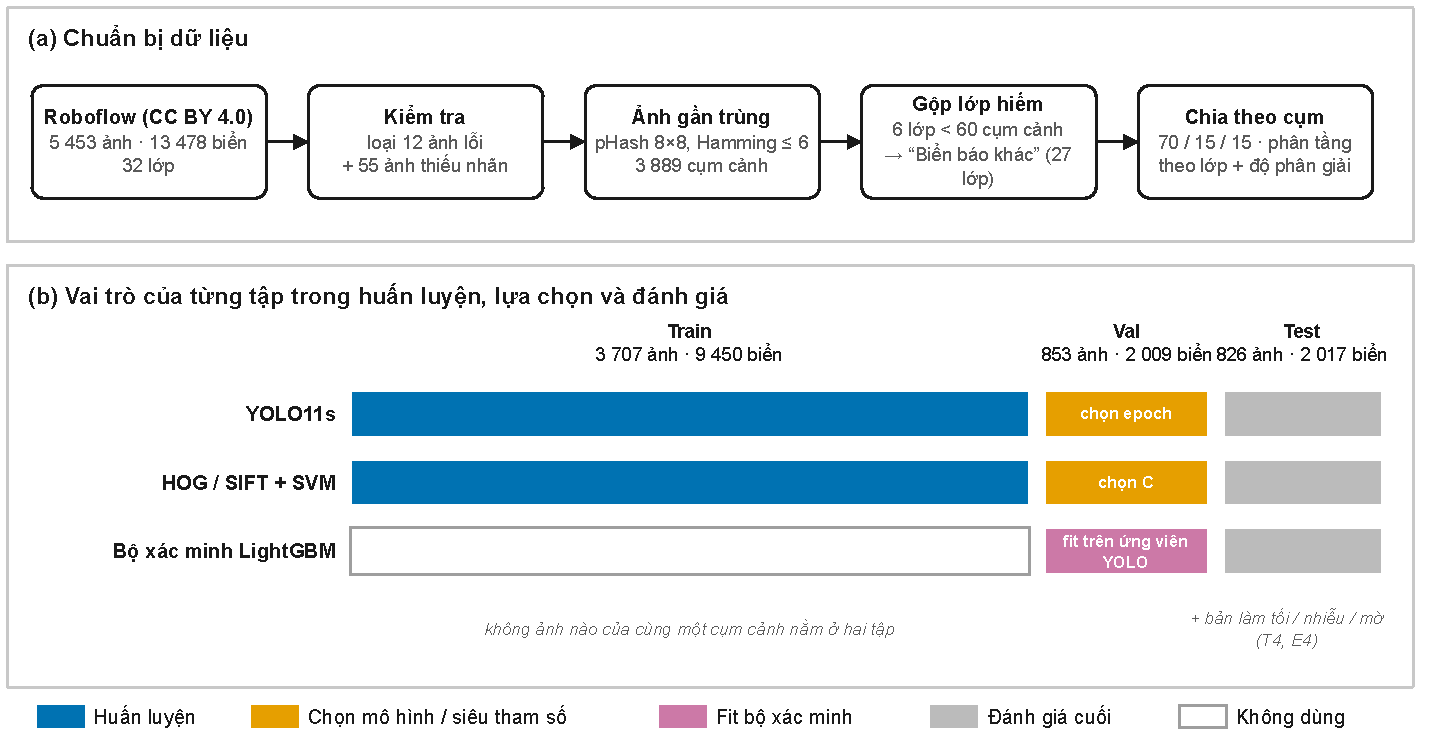
\includegraphics[width=\textwidth]{figures/Fig_du_lieu.pdf}
\caption[Chuẩn bị dữ liệu và vai trò của từng tập]{Chuẩn bị dữ liệu (a) và vai trò của từng tập đối với các mô hình (b)}
\label{fig:data_flow}
\fignote{Độ rộng thanh tỉ lệ với số ảnh (Val và Test được nới tối thiểu để đọc được nhãn).}
\end{figure}

Bảng~\ref{tab:split} cho số ảnh và số biển sau khi chia. Hình~\ref{fig:data_flow}b cho biết mỗi tập được dùng vào việc gì: tập huấn luyện để học tham số, tập xác thực để chọn epoch của YOLO, chọn tham số $C$ của SVM và học bộ xác minh; tập kiểm thử chỉ dùng cho đánh giá cuối và không tham gia bất kỳ lựa chọn nào.

\begin{table}[H]
\centering
\caption{Thống kê bộ dữ liệu sau khi chia theo cụm}
\label{tab:split}
\small
\begin{tabularx}{\textwidth}{|>{\raggedright\arraybackslash}X|>{\centering\arraybackslash}p{2.2cm}|>{\centering\arraybackslash}p{2.2cm}|>{\centering\arraybackslash}p{2.2cm}|>{\centering\arraybackslash}p{2.2cm}|}
\toprule
 & \textbf{Train} & \textbf{Val} & \textbf{Test} & \textbf{Tổng} \\
\midrule
Số ảnh & 3\,707 & 853 & 826 & 5\,386 \\ \hline
Số biển (khung bao) & 9\,450 & 2\,009 & 2\,017 & 13\,476 \\ \hline
Tỉ lệ ảnh (\%) & 68,8 & 15,8 & 15,3 & 100 \\
\bottomrule
\end{tabularx}
\tablenote{53 ảnh không có biển được giữ làm ảnh nền.}
\end{table}

\subsection{Phân tích khám phá dữ liệu}
\label{sec:data_eda}
Hình~\ref{fig:eda_size} và Hình~\ref{fig:eda_class} tóm tắt các đặc điểm ảnh hưởng trực tiếp đến thiết kế:
\begin{itemize}
 \item Biển rất nhỏ. Cạnh tương đương trung vị là 30~px; 18,3\% số biển nhỏ hơn 16~px và 53,7\% nhỏ hơn 32~px. Một số lớp có tới 38--48\% số biển dưới 16~px (Cấm đi ngược chiều, Phải đi vòng sang bên phải, Giới hạn chiều cao, Vạch sang đường cho người đi bộ).
 \item Bốn độ phân giải. $960\times540$ (2\,346 ảnh), $1622\times626$ (2\,213 ảnh, nguồn Zalo), $1920\times1080$ (798 ảnh) và $540\times960$ (29 ảnh). Ảnh $1622\times626$ có nhiều biển nhỏ ở xa.
 \item Mất cân bằng lớp. Nhiều nhất là Giới hạn tốc độ (1\,705 biển), ít nhất là Chỗ quay xe (76 biển), chênh 22 lần; trước khi gộp là 55 lần. Biển cấm chiếm 57\% số biển.
 \item Nhiều biển trên một ảnh. Trung bình 2,5 biển mỗi ảnh; 73 ảnh có từ 10 biển trở lên.
\end{itemize}

\begin{figure}[H]
\centering
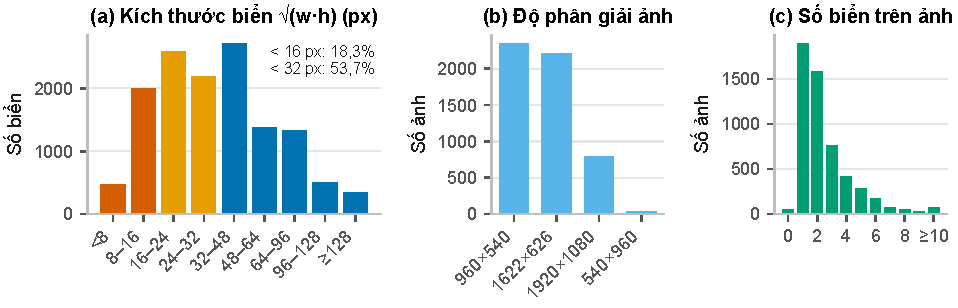
\includegraphics[width=\textwidth]{figures/ch2_eda_kich_thuoc.pdf}
\caption{Phân bố kích thước biển, độ phân giải ảnh và số biển trên mỗi ảnh}
\label{fig:eda_size}
\fignote{Cột đỏ: biển $<16$~px; cột cam: $16$--$32$~px.}
\end{figure}

\begin{figure}[H]
\centering
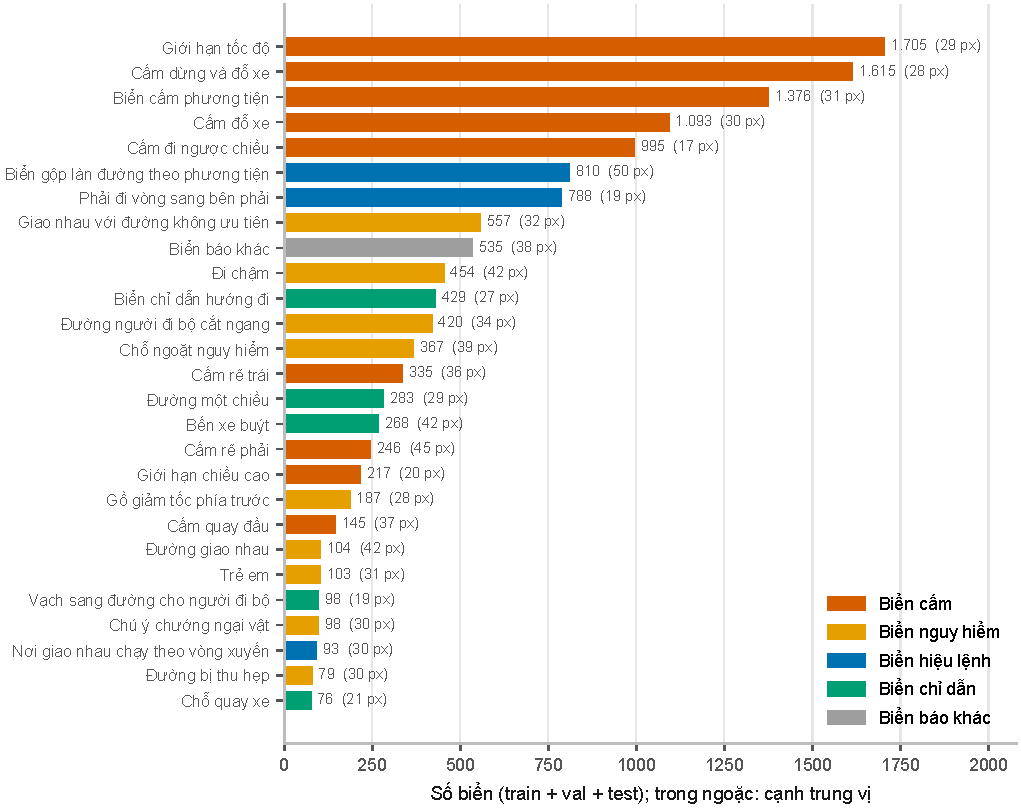
\includegraphics[width=.92\textwidth]{figures/ch2_eda_lop.pdf}
\caption{Số biển của 27 lớp theo nhóm biển; trong ngoặc là cạnh tương đương trung vị}
\label{fig:eda_class}
\end{figure}

\subsection{Dữ liệu chữ và video}
Nhãn lớp và khung bao không đủ để đo khả năng đọc nội dung: cần bản chép đúng của giá trị số và chữ, kể cả dấu tiếng Việt. Vì dữ liệu được đóng băng, đề tài không có nhãn chữ; khả năng đọc chữ chỉ được đánh giá định tính trên ảnh của tập kiểm thử. Video chỉ dùng để minh hoạ chức năng theo vết; ghép ảnh tĩnh thành video không hợp lệ cho việc đo độ ổn định nhãn vì cảnh thay đổi sau mỗi vài khung hình.

\section{Kiến trúc tổng thể}
\label{sec:architecture}

Hình~\ref{fig:system_pipeline} là kiến trúc của hệ thống chính, được dùng chung cho API ảnh, xử lý video nền và webcam~\cite{utci_thietke}. Mỗi khâu được gắn nhãn theo loại phương pháp: CV cho xử lý ảnh và đặc trưng thủ công, DL cho học sâu. Mỗi khâu có cờ bật/tắt trong tệp cấu hình để đo đóng góp riêng.

\begin{figure}[H]
\centering
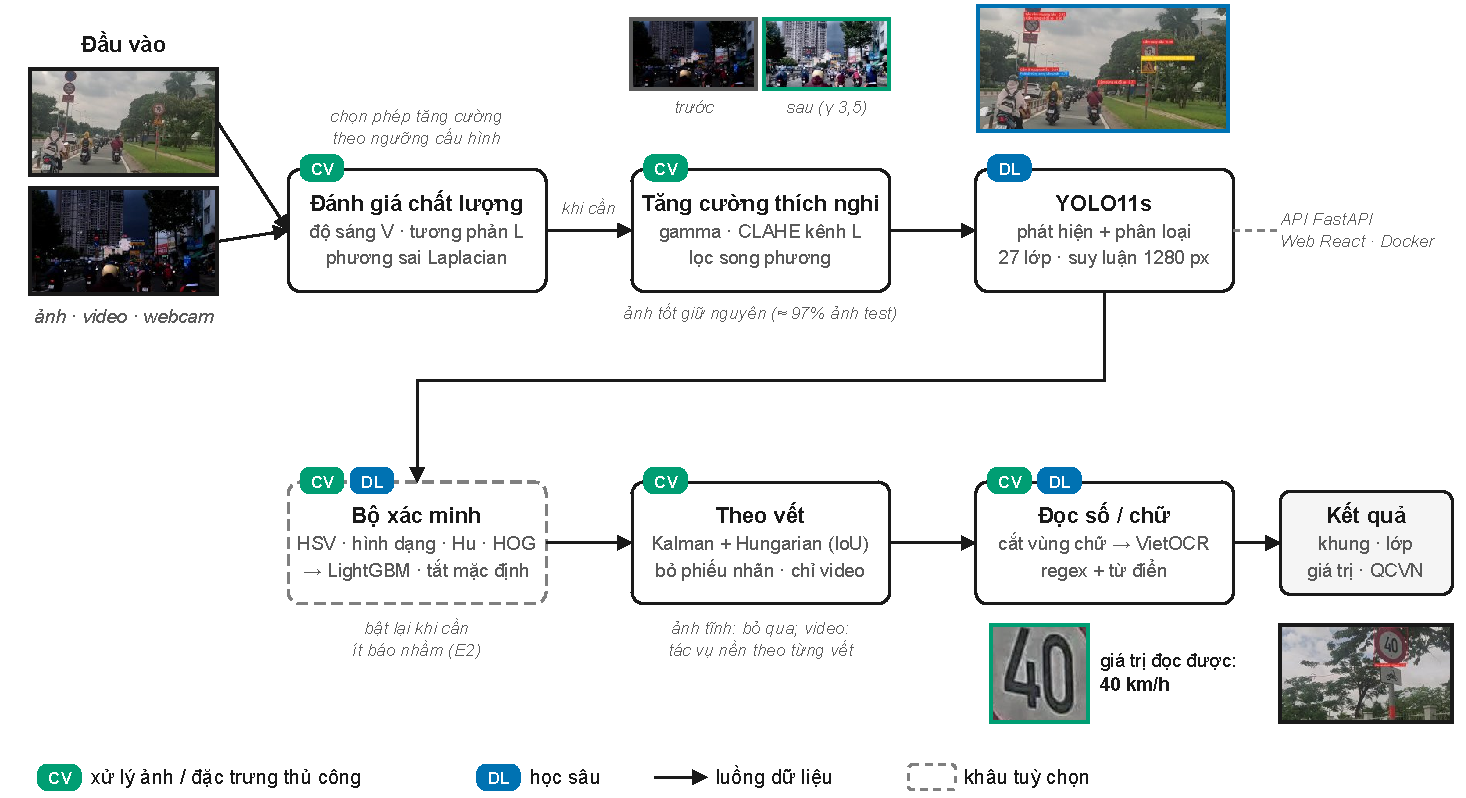
\includegraphics[width=\textwidth]{figures/Fig_pipeline_he_thong.pdf}
\caption[Kiến trúc hệ thống nhận diện biển báo]{Kiến trúc hệ thống nhận diện biển báo: đánh giá chất lượng và tăng cường thích nghi [CV] $\rightarrow$ YOLO11s [DL] $\rightarrow$ bộ xác minh (tuỳ chọn) $\rightarrow$ theo vết [CV] $\rightarrow$ đọc số, chữ [CV + DL]}
\label{fig:system_pipeline}
\fignote{Ảnh nhỏ là kết quả trung gian thật của hệ thống trên ảnh thuộc tập kiểm thử.}
\end{figure}

Luồng xử lý một khung hình gồm năm bước:
\begin{enumerate}
 \item Đánh giá chất lượng [CV]: đo độ sáng, tương phản và độ nét trên ảnh thu nhỏ; chỉ khi các chỉ báo vượt ngưỡng mới tăng cường. Ảnh tốt đi thẳng qua.
 \item Phát hiện và phân loại [DL]: YOLO11s trả khung bao, lớp và điểm tin cậy cho 27 lớp.
 \item Xác minh [CV + DL, tuỳ chọn]: LightGBM trên đặc trưng thủ công và ngữ cảnh YOLO đánh giá lại từng phát hiện. Khâu này tắt mặc định dựa trên kết quả thử nghiệm (Mục~\ref{sec:t1}).
 \item Theo vết [CV]: với video, ghép phát hiện qua các khung hình bằng Kalman và Hungarian, bỏ phiếu nhãn theo vết.
 \item Đọc số, chữ [CV + DL]: cắt vùng chữ bằng xử lý ảnh, đọc bằng VietOCR, kiểm tra bằng biểu thức chính quy và từ điển; ghép với thông tin QCVN của lớp để trả kết quả.
\end{enumerate}
Với ảnh tĩnh, các khâu chạy tuần tự. Với video, xác minh và đọc chữ chạy nền theo từng vết (khi vết mới xuất hiện hoặc sau mỗi 10 khung hình), nên không chặn luồng phát hiện.

Song song với hệ thống chính, nhóm xây dựng một hệ thống đối chứng chỉ dùng thị giác máy tính truyền thống (Mục~\ref{sec:cv_pipeline}). Hệ thống đối chứng không dùng trong sản phẩm; nó dùng để so sánh hai phương pháp trên cùng ảnh và cùng tập kiểm thử (Chương~\ref{chap:chuong3}).

\section{Phương pháp học sâu}
\label{sec:deep}

\subsection{Mô hình phát hiện YOLO11s}
Nhóm chọn YOLO11 của Ultralytics~\cite{ultralytics_yolo11,khanam2024yolo11}, biến thể nhỏ YOLO11s, khởi tạo từ trọng số học trên COCO~\cite{lin2014coco} rồi tinh chỉnh toàn bộ mạng trên tập huấn luyện. Một mô hình đảm nhiệm cả tìm vị trí và phân loại, nên hệ thống không cần mạng phân loại biển riêng. Bảng~\ref{tab:ch2_detector_config} là cấu hình dùng cho lần huấn luyện được chọn~\cite{utci_cauhinh}.

\begin{table}[H]
\centering
\caption{Cấu hình huấn luyện và suy luận của YOLO11s}
\label{tab:ch2_detector_config}
\small
\begin{tabularx}{\textwidth}{|>{\raggedright\arraybackslash}p{3.6cm}|>{\raggedright\arraybackslash}X|}
\toprule
\textbf{Thành phần} & \textbf{Giá trị} \\
\midrule
Trọng số khởi tạo & YOLO11s đã huấn luyện trước trên COCO \\ \hline
Kích thước ảnh huấn luyện & 960 px (cạnh dài), giữ tỉ lệ và đệm theo thư viện \\ \hline
Số epoch, kích thước lô & 80 epoch; 8 ảnh mỗi lô \\ \hline
Tối ưu & AdamW, tốc độ học ban đầu $0{,}001$, lịch cosine, 3 epoch khởi động \\ \hline
Tăng cường dữ liệu & Mặc định của thư viện; tắt lật ngang (tránh đổi nghĩa biển trái--phải); tắt mosaic ở 15 epoch cuối \\ \hline
Chọn trọng số & Epoch có mAP@50:95 cao nhất trên tập xác thực \\ \hline
Môi trường & Google Colab, Tesla T4; Ultralytics 8.4.183; 2 giờ 52 phút \\ \hline
Suy luận & 1280 px (chọn theo thí nghiệm T3), ngưỡng điểm $0{,}25$, NMS với IoU $0{,}5$, FP16 trên GPU \\
\bottomrule
\end{tabularx}
\end{table}

Mô hình được huấn luyện ở 960 px nhưng suy luận ở 1280 px. Phóng to ảnh khi suy luận làm biển nhỏ chiếm nhiều điểm ảnh hơn trên bản đồ đặc trưng mà không cần huấn luyện lại; thí nghiệm T3 (Mục~\ref{sec:t3}) cho thấy cách này tăng recall biển nhỏ mà không giảm precision. Hệ thống cũng có tuỳ chọn cắt ô $640\times640$ chồng lấn theo ý tưởng SAHI~\cite{akyon2022sahi} cho ảnh độ phân giải cao.

\subsection{Đọc chữ và giá trị số}
Nhận dạng ký tự quang học (OCR) gồm bước tìm vùng chữ và bước nhận dạng nội dung (Hình~\ref{fig:ocr_basic})~\cite{paddleocr_overview}. Hệ thống tách hai bước theo hai loại phương pháp: vùng chữ được cắt bằng xử lý ảnh [CV], nội dung được đọc bằng VietOCR với cấu hình VGG-Transformer (trích đặc trưng VGG, giải mã Transformer) [DL]~\cite{vietocr_repo}.

\begin{figure}[H]
\centering
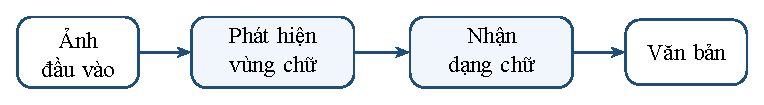
\includegraphics[width=.9\textwidth]{figures/fig_1_6_ocr.pdf}
\caption[Kiến trúc OCR cơ bản]{Kiến trúc OCR cơ bản: phát hiện vùng chữ và nhận dạng nội dung}
\label{fig:ocr_basic}
\end{figure}

\begin{itemize}
 \item Biển có giá trị số (tốc độ, chiều cao): cắt đĩa phía trong viền đỏ (78\% đường kính), phóng to 3 lần, yêu cầu chiều cao vùng tối thiểu 40~px.
 \item Dòng chữ và biển phụ: tìm tấm chữ nhật sáng phía dưới biển chính (vùng tìm cao 1,2 lần biển chính), tách dòng bằng chiếu histogram theo hàng, tăng tương phản bằng CLAHE và chỉnh nghiêng trước khi đọc.
 \item Hậu xử lý: biểu thức chính quy tách số và đơn vị; giá trị tốc độ phải thuộc danh sách hợp lệ (5--120 km/h), chiều cao trong khoảng 1,5--6 m; chữ được so với từ điển bằng độ tương đồng chuỗi (ngưỡng 80/100). Dòng có độ tin cậy VietOCR dưới 0,75 bị bỏ.
\end{itemize}
Chuỗi gốc và chuỗi sau xử lý đều được lưu. Quy tắc sửa không được ``đoán'': nếu ảnh chưa phân biệt được 50 và 60, danh sách giá trị hợp lệ không đủ căn cứ để chọn, và kết quả để trống. Với video, vùng đọc được chọn từ khung hình có tích diện tích và độ nét lớn nhất của vết.

\section{Phương pháp thị giác máy tính truyền thống}
\label{sec:classic}

\subsection{Đánh giá chất lượng và tăng cường ảnh thích nghi}
\label{sec:enhance}
Ảnh được thu nhỏ về chiều rộng 320 px rồi đo ba chỉ báo: độ sáng trung bình $\mu_V$ của kênh V (HSV), độ lệch chuẩn $\sigma_L$ của kênh L (Lab) và phương sai đáp ứng Laplacian $\sigma^2_{\nabla^2}$ trên ảnh xám. Tập phép tăng cường được chọn theo quy tắc:
\begin{equation}
 \mathcal{O}=
 \begin{cases}
  \{\text{gamma},\text{CLAHE}\} & \text{nếu } \mu_V<0{,}30,\\
  \{\text{CLAHE}\} & \text{nếu } \sigma_L<0{,}13,\\
  \{\text{lọc song phương}\} & \text{nếu } \sigma^2_{\nabla^2}>4000,
 \end{cases}
 \label{eq:enhance_rule}
\end{equation}
(lấy hợp của các điều kiện thoả mãn). Các ngưỡng được chọn từ thống kê dữ liệu ở Sprint 1, trước khi có tập kiểm thử của các thí nghiệm; ảnh không thoả điều kiện nào được giữ nguyên.

Gamma tự động đưa độ sáng trung bình về $0{,}5$:
\begin{equation}
 \gamma=\operatorname{clip}\!\left(\frac{\ln\mu_V}{\ln0{,}5},\,0{,}4,\,3{,}0\right),\qquad
 I'(x,y)=255\left(\frac{I(x,y)}{255}\right)^{1/\gamma}.
 \label{eq:gamma}
\end{equation}
Với ảnh tối ($\mu_V<0{,}5$) ta có $\gamma>1$, nên số mũ $1/\gamma<1$ làm sáng ảnh. CLAHE~\cite{zuiderveld1994clahe} được áp trên kênh L của không gian Lab (giới hạn tương phản 2,0, lưới $8\times8$), tăng tương phản cục bộ mà không làm lệch màu đỏ, xanh, vàng của biển. Lọc song phương~\cite{tomasi1998bilateral} (đường kính 5, $\sigma_{\text{màu}}=\sigma_{\text{không gian}}=50$) giảm nhiễu nhưng giữ biên. Thiết kế ``chỉ tăng cường khi cần'' xuất phát từ quan sát rằng áp dụng mọi phép cho mọi ảnh có thể làm hại ảnh tốt hoặc ảnh nhiễu; thí nghiệm T4 (Mục~\ref{sec:t4}) kiểm chứng điều này.

\subsection{Pipeline đối chứng: màu, hình dạng, HOG và SVM}
\label{sec:cv_pipeline}
Pipeline đối chứng giải toàn bộ bài toán phát hiện và phân loại mà không dùng mạng nơ-ron (Hình~\ref{fig:cv_pipeline}). Nó kế thừa hướng màu--hình dạng của các công trình kinh điển~\cite{escalera1997road,maldonado2007svm} và đặc trưng HOG~\cite{dalal2005hog}.

\begin{figure}[H]
\centering
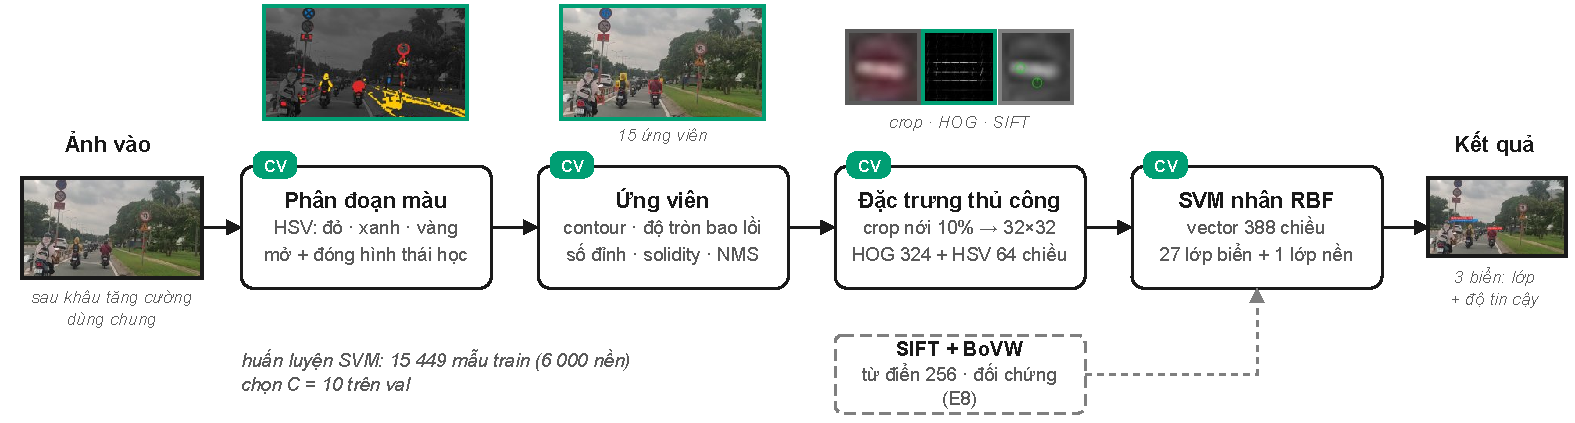
\includegraphics[width=\textwidth]{figures/Fig_pipeline_cv.pdf}
\caption[Pipeline CV truyền thống đối chứng]{Pipeline CV truyền thống đối chứng: phân đoạn màu HSV $\rightarrow$ ứng viên theo hình dạng $\rightarrow$ HOG + histogram HSV $\rightarrow$ SVM có lớp nền}
\label{fig:cv_pipeline}
\end{figure}

\paragraph{Phân đoạn màu.} Ảnh được chuyển sang HSV và lấy ngưỡng theo ba màu quy chuẩn: đỏ (hai dải $H\in[0,10]\cup[160,179]$ vì sắc đỏ nằm ở hai đầu vòng màu, $S\ge70$, $V\ge50$), xanh ($H\in[95,130]$) và vàng ($H\in[15,35]$). Mỗi mặt nạ được mở rồi đóng bằng phần tử cấu trúc $3\times3$ để bỏ điểm nhiễu và nối viền bị đứt.

\paragraph{Ứng viên theo hình dạng.} Với mỗi đường bao ngoài có diện tích từ 60~px$^2$ đến 25\% ảnh, hệ thống tính tỉ lệ khung $a=w/h$, số đỉnh $k$ sau xấp xỉ đa giác (sai số $0{,}04$ chu vi), độ đặc $\rho=A/A_{\text{bao lồi}}$ và độ tròn của bao lồi
\begin{equation}
 C_{\text{hull}}=\frac{4\pi A_{\text{hull}}}{P_{\text{hull}}^2}.
 \label{eq:hull_circularity}
\end{equation}
Viền đỏ của biển cấm là một vòng rỗng nên độ tròn của chính đường bao thấp; dùng bao lồi khắc phục điều này. Vùng được nhận là \textit{tròn} nếu $0{,}6\le a\le1{,}6$ và $C_{\text{hull}}\ge0{,}75$; \textit{tam giác} nếu màu đỏ hoặc vàng, $k=3$, $0{,}7\le a\le1{,}5$, $\rho>0{,}6$; \textit{chữ nhật} nếu màu xanh, $4\le k\le6$, $0{,}5\le a\le3$, $\rho>0{,}8$. Các ứng viên trùng nhau được loại bằng NMS (IoU $0{,}3$) và loại mảnh màu nằm trong một biển lớn hơn.

\paragraph{Đặc trưng thủ công.} Mỗi ứng viên được cắt nới 10\% mỗi phía và đưa về $32\times32$. HOG trên ảnh xám dùng 9 hướng, ô $8\times8$, khối $2\times2$, cho vector 324 chiều mô tả ký hiệu bên trong biển. Histogram HSV $16\times4$ (16 mức sắc độ, 4 mức bão hoà) chuẩn hoá tổng bằng 1, cho 64 chiều mô tả màu. Vector ghép có 388 chiều. Hai loại đặc trưng bổ sung cho nhau: HOG trên ảnh xám bỏ qua màu, trong khi màu lại là thông tin quy chuẩn phân biệt biển cấm, nguy hiểm và hiệu lệnh.

\paragraph{Phân loại bằng SVM.} SVM nhân RBF~\cite{cortes1995svm} sau bước chuẩn hoá đặc trưng phân loại 28 lớp: 27 lớp biển và một lớp \textit{nền}. Mẫu nền là các ứng viên màu--hình dạng trên ảnh huấn luyện không trùng biển thật nào (IoU $<0{,}1$); nhờ lớp này, SVM loại được vùng màu giả như áo, xe, mái tôn. Tập huấn luyện có 15\,449 mẫu (6\,000 nền), trọng số lớp cân bằng; $C\in\{1,10\}$ được chọn trên tập xác thực (3\,509 mẫu), kết quả $C=10$. Ứng viên có xác suất dưới 0,30 không được hiển thị. Hình~\ref{fig:cv_steps} minh hoạ các bước trên một ảnh của tập kiểm thử.

\begin{figure}[H]
\centering
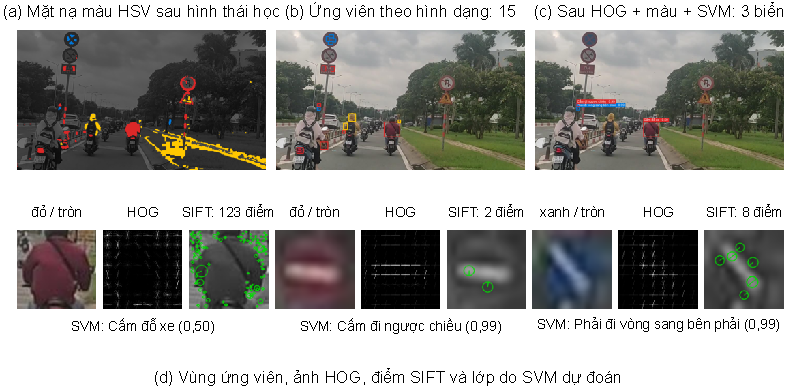
\includegraphics[width=\textwidth]{figures/ch2_cv_buoc.pdf}
\caption{Các bước của pipeline CV truyền thống trên một ảnh của tập kiểm thử}
\label{fig:cv_steps}
\fignote{Vùng thứ nhất ở (d) là áo đỏ bị nhận nhầm thành ``Cấm đỗ xe'' với xác suất 0,50 --- một dạng báo động giả điển hình của hướng màu--hình dạng.}
\end{figure}

\paragraph{SIFT kết hợp túi từ thị giác (đối chứng âm).} Để kiểm chứng việc chọn HOG, nhóm cài thêm SIFT~\cite{lowe2004sift} trên vùng biển phóng về $64\times64$, lượng tử hoá thành từ điển 256 từ bằng k-means (MiniBatch) và biểu diễn mỗi vùng bằng histogram từ~\cite{csurka2004bovw}, sau đó dùng cùng SVM. Biển báo có ít kết cấu, nên dự kiến SIFT sẽ kém HOG; thí nghiệm E8 kiểm chứng dự kiến này.

\subsection{Bộ xác minh}
\label{sec:verifier}
Bộ xác minh đánh giá lại một phát hiện của YOLO bằng đặc trưng thủ công của vùng đó. Với vùng $b_j$, lớp $c_j$ và điểm $s_j^{\mathrm{det}}$:
\begin{equation}
 z_j=\varphi(I,b_j,c_j,s_j^{\mathrm{det}}),\qquad
 q_j=g_{\psi}(z_j).
 \label{eq:verifier_problem}
\end{equation}
Hàm $\varphi$ trích vector $z_j$ gồm ngữ cảnh YOLO (điểm, lớp, kích thước, vị trí), tỉ lệ màu HSV, đặc trưng hình học, bảy moment Hu~\cite{hu1962moments} và HOG giảm chiều bằng PCA (16 thành phần); $g_\psi$ là LightGBM~\cite{ke2017lightgbm} (400 cây, tốc độ học $0{,}05$, 31 lá, cân bằng lớp) kèm hiệu chỉnh xác suất isotonic. Nhãn huấn luyện lấy từ các phát hiện của YOLO trên tập xác thực với ngưỡng thấp $0{,}10$: phát hiện đúng lớp và có IoU $\ge0{,}5$ với một biển thật là mẫu dương, còn lại là mẫu âm. Ý tưởng này theo hướng ``theo vết rồi lọc bằng mô hình phân biệt riêng'' của Šegvić và cộng sự~\cite{segvic2014temporal}. Thí nghiệm T1 cho thấy bộ xác minh không vượt được điểm tin cậy của chính YOLO, nên khâu này được tắt mặc định (Mục~\ref{sec:t1}).

\subsection{Theo vết và tổng hợp nhãn}
Theo vết liên kết các phát hiện của cùng một biển qua nhiều khung hình theo cách của SORT~\cite{bewley2016sort}. Bộ lọc Kalman~\cite{kalman1960filter} ước lượng trạng thái 8 chiều gồm tâm $(c_x,c_y)$, kích thước $(w,h)$ của khung và vận tốc biến đổi của bốn đại lượng này trên ảnh; bước dự đoán ước lượng vị trí ở khung tiếp theo, bước cập nhật kết hợp dự đoán với phát hiện mới. Phát hiện mới được ghép với vết đang có bằng thuật toán Hungarian~\cite{kuhn1955hungarian} sao cho tổng IoU giữa khung dự đoán và khung phát hiện lớn nhất; cặp có IoU dưới $0{,}3$ bị loại.

Vết được xác nhận sau 3 lần quan sát và bị xoá sau 15 khung hình không xuất hiện lại. Nhãn hiển thị của vết là lớp có tổng điểm lớn nhất trong cửa sổ 10 quan sát gần nhất, giúp giảm hiện tượng nhãn nhảy giữa các khung do mờ hoặc che khuất. Cửa sổ dài làm nhãn ổn định hơn nhưng chậm sửa một nhãn sai. Các đại lượng của bộ lọc mô tả chuyển động biểu kiến trên ảnh, không phải tốc độ hay khoảng cách vật lý của biển.

\section{Tổ chức huấn luyện và đánh giá}
\label{sec:protocol}

\subsection{Huấn luyện riêng từng mô hình}
Bốn mô hình được huấn luyện riêng với dữ liệu và mục tiêu khác nhau (Hình~\ref{fig:data_flow}b): YOLO11s trên ảnh huấn luyện; SVM của pipeline đối chứng trên vùng cắt từ ảnh huấn luyện; bộ xác minh trên phát hiện của YOLO ở tập xác thực; VietOCR dùng trọng số huấn luyện trước, không tinh chỉnh. Mỗi lần huấn luyện và mỗi lần đánh giá được ghi vào sổ đăng ký thí nghiệm gồm mã thí nghiệm, commit, cấu hình, môi trường và kết quả, để mọi con số trong Chương~\ref{chap:chuong3} truy được về một lần chạy cụ thể.

\subsection{Các chỉ số đánh giá phát hiện biển báo}
\label{sec:detection_metrics}
Độ giao trên hợp (IoU) đo mức chồng lấn giữa khung dự đoán $B_p$ và khung đúng $B_g$:
\begin{equation}
 \operatorname{IoU}(B_p,B_g)=\frac{|B_p\cap B_g|}{|B_p\cup B_g|}.
 \label{eq:iou}
\end{equation}
Tại một ngưỡng điểm và ngưỡng IoU, dự đoán đúng lớp và khớp với một nhãn thật chưa ghép là phát hiện đúng (TP); dự đoán sai lớp, không khớp hoặc trùng lặp là phát hiện sai (FP); biển thật chưa được phát hiện là bỏ sót (FN):
\begin{equation}
 \operatorname{P}=\frac{TP}{TP+FP},\qquad
 \operatorname{R}=\frac{TP}{TP+FN},\qquad
 F_1=\frac{2\,\mathrm{P}\,\mathrm{R}}{\mathrm{P}+\mathrm{R}}.
 \label{eq:precision_recall}
\end{equation}
Thay đổi ngưỡng điểm tạo đường precision--recall; AP tóm tắt đường này cho một lớp, mAP lấy trung bình giữa $C$ lớp~\cite{tailieu_bai9}:
\begin{equation}
 \operatorname{mAP}_{\tau}=\frac{1}{C}\sum_{c=1}^{C}AP_{c,\tau},\qquad
 \operatorname{mAP}_{50:95}=\frac{1}{10}\sum_{j=0}^{9}\operatorname{mAP}_{0.50+0.05j}.
 \label{eq:map}
\end{equation}
mAP@50 dùng ngưỡng IoU $0{,}5$; mAP@50:95 xét các ngưỡng từ $0{,}5$ đến $0{,}95$ nên đòi hỏi khung khớp chặt hơn~\cite{coco_evaluation,ultralytics_metrics}.

\subsection{Giao thức đánh giá}
Để kết quả phản ánh đúng hệ thống khi chạy thật và so sánh được giữa các cấu hình, nhóm cố định giao thức sau:
\begin{itemize}
 \item Điểm vận hành. Chỉ số chính là P, R, $F_1$ tại ngưỡng hiển thị của hệ thống (điểm $0{,}25$), đúng lớp và IoU $\ge0{,}5$. Precision ở ngưỡng tối ưu theo $F_1$ do thư viện báo cáo không phải điều người dùng nhìn thấy. Ma trận nhầm lẫn mặc định của Ultralytics~8.4 ghép cả dự đoán điểm $0{,}001$ nên không được dùng làm bằng chứng.
 \item Theo kích thước và theo lớp. Recall được tính riêng cho bốn nhóm kích thước và cho từng lớp, vì giá trị trung bình che lấp điểm yếu ở biển nhỏ và lớp hiếm.
 \item Khoảng tin cậy. CI 95\% của chỉ số toàn tập được ước lượng bằng bootstrap theo ảnh~\cite{efron1993bootstrap} (500--2\,000 lần lấy mẫu lặp; ghép cặp khi so hai cấu hình trên cùng ảnh); CI của tỉ lệ theo lớp dùng khoảng Wilson~\cite{wilson1927}. Hai cấu hình chỉ được coi là khác nhau khi CI của hiệu không chứa 0.
 \item Mức tương đồng với tập huấn luyện. Ảnh kiểm thử được chia ba nhóm theo khoảng cách pHash tới ảnh huấn luyện gần nhất ($\le10$, 11--14, $\ge15$ bit). Nhóm ``khác train'' cho ước lượng gần hơn với ảnh mới, thay cho tập ngoài phân phối mà đề tài không có.
 \item Ảnh xấu giả lập. Ảnh tối: $I'=255\,(I/255)^{\gamma}$ với $\gamma=2{,}5$ hoặc $3{,}5$; nhiễu Gauss $\sigma=15$; mờ chuyển động ngang với nhân 9~px.
 \item Tốc độ. Ghi rõ phần cứng, kích thước ảnh và các khâu được tính thời gian.
\end{itemize}

\subsection{Các thí nghiệm}
Bảng~\ref{tab:experiments} liệt kê các thí nghiệm, câu hỏi mỗi thí nghiệm trả lời và mục trình bày kết quả.

\begin{table}[H]
\centering
\caption{Danh sách thí nghiệm}
\label{tab:experiments}
\small
\begin{tabularx}{\textwidth}{|>{\centering\arraybackslash}p{1.1cm}|>{\raggedright\arraybackslash}X|>{\raggedright\arraybackslash}p{4.4cm}|>{\centering\arraybackslash}p{1.5cm}|}
\toprule
\textbf{Mã} & \textbf{Câu hỏi} & \textbf{Thiết kế} & \textbf{Mục} \\
\midrule
S1 & YOLO11s học tốt đến đâu trên dữ liệu cùng nguồn? & Huấn luyện 960 px; mAP, CI bootstrap, theo lớp, kích thước, tương đồng & \ref{sec:baseline} \\ \hline
T0, T1 & Đặc trưng thủ công có giúp loại phát hiện sai của YOLO? & Ablation tập đặc trưng của bộ xác minh; P ở cùng recall & \ref{sec:t1} \\ \hline
T3 & Tăng recall biển nhỏ mà không huấn luyện lại? & Suy luận 960 / 1280 / cắt ô 640 & \ref{sec:t3} \\ \hline
T4, E4 & Tăng cường thích nghi có giúp khi ảnh xấu? & Ảnh tối, nhiễu, mờ; không xử lý / thích nghi / luôn áp & \ref{sec:t4} \\ \hline
E8 & Đặc trưng thủ công + SVM so với YOLO ở phân loại? & Cùng 2\,017 biển; theo kích thước; ghép cặp & \ref{sec:e8} \\ \hline
E1, E2 & Hệ thống mặc định đạt bao nhiêu; mỗi khâu đóng góp gì? & Cấu hình mặc định; ablation bật từng khâu & \ref{sec:e1} \\
\bottomrule
\end{tabularx}
\end{table}

\subsection{Đánh giá đọc chữ, tốc độ và độ ổn định}
Khả năng đọc chữ nên được đo bằng tỉ lệ lỗi ký tự $\operatorname{CER}=(S+D+I)/N$ và tỉ lệ khớp hoàn toàn~\cite{torchmetrics_cer}, trong đó $S,D,I$ là số phép thay, xoá, chèn và $N$ là độ dài chuỗi tham chiếu. Do không có nhãn chữ, đề tài chỉ đánh giá định tính. Số khung hình mỗi giây $\mathrm{FPS}=n/T$ và độ trễ từ lúc nhận ảnh đến lúc có kết quả được đo riêng cho khâu phát hiện, cho API ảnh và cho luồng WebSocket. Với video, độ ổn định nhãn được định nghĩa là tỉ lệ khung hình mà nhãn hiển thị của cùng một vết bị đổi; công cụ đo đã có nhưng chưa có video đường phố thật để đo.

\chapter{KẾT QUẢ THỰC HIỆN BÀI TOÁN}
\label{chap:chuong3}

Chương này trình bày thiết lập thực nghiệm, kết quả huấn luyện YOLO11s, các thí nghiệm về biển nhỏ, ảnh xấu, so sánh phương pháp truyền thống với học sâu, bộ xác minh, kết quả của hệ thống đầy đủ, tốc độ, chương trình demo và phần thảo luận. Mọi con số được tính bằng script của dự án từ các lần chạy đã ghi trong sổ đăng ký thí nghiệm; các biểu đồ được sinh tự động từ cùng tệp số liệu, không có con số nào chép tay. Trừ khi ghi khác, kết quả được đo trên tập kiểm thử \texttt{processed/v1} (826 ảnh, 2\,017 biển) theo giao thức ở Mục~\ref{sec:protocol}.

\section{Thiết lập thực nghiệm}
\label{sec:setup}

Bảng~\ref{tab:env} tóm tắt môi trường. YOLO11s được huấn luyện một lần (hạt giống 42) trên Google Colab; mọi đánh giá và đo tốc độ chạy trên máy cá nhân của nhóm. Dữ liệu, trọng số và cấu hình của từng lần chạy được ghi lại để tái lập (Phụ lục~\ref{app:code}).

\begin{table}[H]
\centering
\caption{Môi trường thực nghiệm}
\label{tab:env}
\small
\begin{tabularx}{\textwidth}{|>{\raggedright\arraybackslash}p{3.4cm}|>{\raggedright\arraybackslash}X|}
\toprule
\textbf{Hạng mục} & \textbf{Giá trị} \\
\midrule
Huấn luyện YOLO11s & Google Colab, GPU Tesla T4; Python 3.13, PyTorch 2.11 + CUDA 13.0, Ultralytics 8.4.183 \\ \hline
Đánh giá, đo tốc độ & Máy tính xách tay, GPU RTX 4060 Laptop; PyTorch + CUDA 12.6 \\ \hline
Triển khai & Docker Compose (profile CPU và GPU), FastAPI, React 19, Nginx \\ \hline
Thư viện CV / ML & OpenCV 4.14, scikit-image (HOG), scikit-learn 1.9 (SVM), LightGBM 4.7, VietOCR \\ \hline
Dữ liệu & \texttt{processed/v1}, 27 lớp; tập kiểm thử chưa dùng cho bất kỳ lựa chọn nào \\
\bottomrule
\end{tabularx}
\end{table}

\section{Kết quả huấn luyện YOLO11s}
\label{sec:baseline}

\subsection{Quá trình hội tụ}
Hình~\ref{fig:training} cho thấy hàm mất mát khung bao và phân loại trên cả tập huấn luyện lẫn tập xác thực giảm đều đến epoch 80; mất mát xác thực không tăng trở lại, nên không có dấu hiệu quá khớp. Bước giảm đột ngột của mất mát huấn luyện quanh epoch 66 là do tắt tăng cường mosaic ở 15 epoch cuối. mAP@50:95 trên tập xác thực tăng từ 0,645 (epoch 30) lên 0,672 (epoch 50) và 0,685 (epoch 80); 15 epoch cuối chỉ thêm 0,003, tức mô hình gần bão hoà trên dữ liệu hiện có. Thời gian huấn luyện là 2 giờ 52 phút.

\begin{figure}[H]
\centering
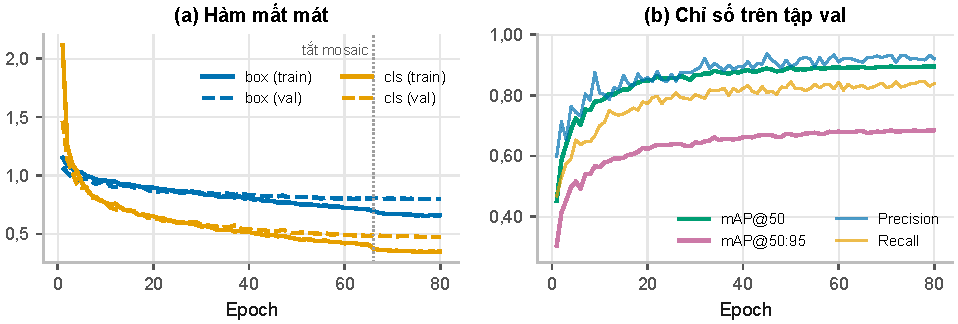
\includegraphics[width=\textwidth]{figures/ch3_huan_luyen.pdf}
\caption{Hàm mất mát (a) và các chỉ số trên tập xác thực (b) của YOLO11s theo epoch}
\label{fig:training}
\end{figure}

\subsection{Kết quả tổng}
Bảng~\ref{tab:baseline} so sánh chỉ số do thư viện báo cáo với chỉ số nhóm tính lại kèm CI 95\% bootstrap 500 lần theo ảnh. Hai cách tính lệch khoảng 0,01 do khác cách đệm ảnh khi suy luận, nên kết quả được báo cáo là mAP@50 $\approx$ 0,89--0,91. Kết quả trên tập xác thực (mAP@50 0,894; mAP@50:95 0,683) tương đương tập kiểm thử, cho thấy việc chọn epoch không quá khớp tập xác thực. Precision 0,920 mà thư viện báo cáo là ở ngưỡng tối ưu theo $F_1$; tại ngưỡng hiển thị $0{,}25$ của hệ thống, precision là 0,860.

\begin{table}[H]
\centering
\caption{Kết quả YOLO11s (suy luận 960 px) trên tập kiểm thử}
\label{tab:baseline}
\small
\begin{tabularx}{\textwidth}{|>{\raggedright\arraybackslash}X|>{\centering\arraybackslash}p{3cm}|>{\centering\arraybackslash}p{3cm}|>{\centering\arraybackslash}p{3.4cm}|}
\toprule
\textbf{Chỉ số} & \textbf{Ultralytics} & \textbf{Tính lại} & \textbf{CI 95\% (bootstrap)} \\
\midrule
mAP@50 & 0,905 & 0,892 & [0,868; 0,917] \\ \hline
mAP@50:95 & 0,684 & 0,676 & [0,657; 0,702] \\ \hline
Precision tại điểm $0{,}25$ & -- & 0,860 & [0,842; 0,878] \\ \hline
Recall tại điểm $0{,}25$ & -- & 0,893 & [0,875; 0,913] \\
\bottomrule
\end{tabularx}
\end{table}

\subsection{Theo kích thước biển}
Bảng~\ref{tab:size_s1} phân tích từng biển thật của tập xác thực và kiểm thử tại ngưỡng $0{,}25$. Với biển từ 16~px trở lên, khoảng 95\% được nhận đúng; lỗi tập trung ở biển dưới 16~px: chỉ 61,7\% được nhận đúng và 32,8\% bị bỏ sót. Nhầm lớp chiếm tỉ lệ nhỏ ở mọi nhóm. Điều này xác định điểm yếu chính của mô hình là \textit{tìm} biển nhỏ, không phải \textit{phân loại} sai.

\begin{table}[H]
\centering
\caption{Kết quả của YOLO11s theo kích thước biển (val + test, ngưỡng $0{,}25$)}
\label{tab:size_s1}
\small
\begin{tabularx}{\textwidth}{|>{\raggedright\arraybackslash}X|>{\centering\arraybackslash}p{2.2cm}|>{\centering\arraybackslash}p{2.2cm}|>{\centering\arraybackslash}p{2.2cm}|>{\centering\arraybackslash}p{2.2cm}|}
\toprule
\textbf{Cạnh biển} & \textbf{Số biển} & \textbf{Đúng lớp} & \textbf{Sai lớp} & \textbf{Bỏ sót} \\
\midrule
$<16$ px & 702 & 0,617 & 0,056 & \textbf{0,328} \\ \hline
$16$--$32$ px & 1\,427 & 0,922 & 0,036 & 0,043 \\ \hline
$32$--$64$ px & 1\,261 & 0,964 & 0,013 & 0,023 \\ \hline
$\ge64$ px & 636 & 0,975 & 0,003 & 0,022 \\
\bottomrule
\end{tabularx}
\end{table}

\subsection{Theo lớp}
Hình~\ref{fig:per_class} cho recall của 27 lớp kèm CI Wilson. 24/27 lớp có recall từ 0,81 trở lên. Ba lớp yếu nhất đều có nguyên nhân xác định:
\begin{itemize}
 \item \textit{Vạch sang đường cho người đi bộ} (recall 0,57, $n=30$) và \textit{Giới hạn chiều cao} (0,68, $n=65$): 57\% và 34\% số biển nhỏ hơn 16~px; với biển từ 16~px trở lên, recall đạt 1,00 và 0,84.
 \item \textit{Biển chỉ dẫn hướng đi} (recall 0,70, precision 0,60): nhãn gốc gộp cả bảng chỉ dẫn chữ nhật lẫn biển tròn xanh, nên định nghĩa lớp không nhất quán; vấn đề nằm ở dữ liệu, không thể sửa vì dữ liệu đã đóng băng.
\end{itemize}
Số lượng dữ liệu tương quan yếu với chất lượng lớp (hệ số Spearman 0,16--0,32 giữa số cụm cảnh và recall/AP). Các lớp hiếm vẫn đạt recall 0,81--0,97 nhưng CI rộng vì chỉ có 23--31 biển để đánh giá. Các cặp nhầm lẫn lớn nhất chỉ chiếm tối đa 6\% số biển của lớp: Biển gộp làn đường $\leftrightarrow$ Biển chỉ dẫn hướng đi, Cấm dừng và đỗ xe $\leftrightarrow$ Cấm đỗ xe, Giới hạn tốc độ $\rightarrow$ Biển cấm phương tiện.

\begin{figure}[H]
\centering
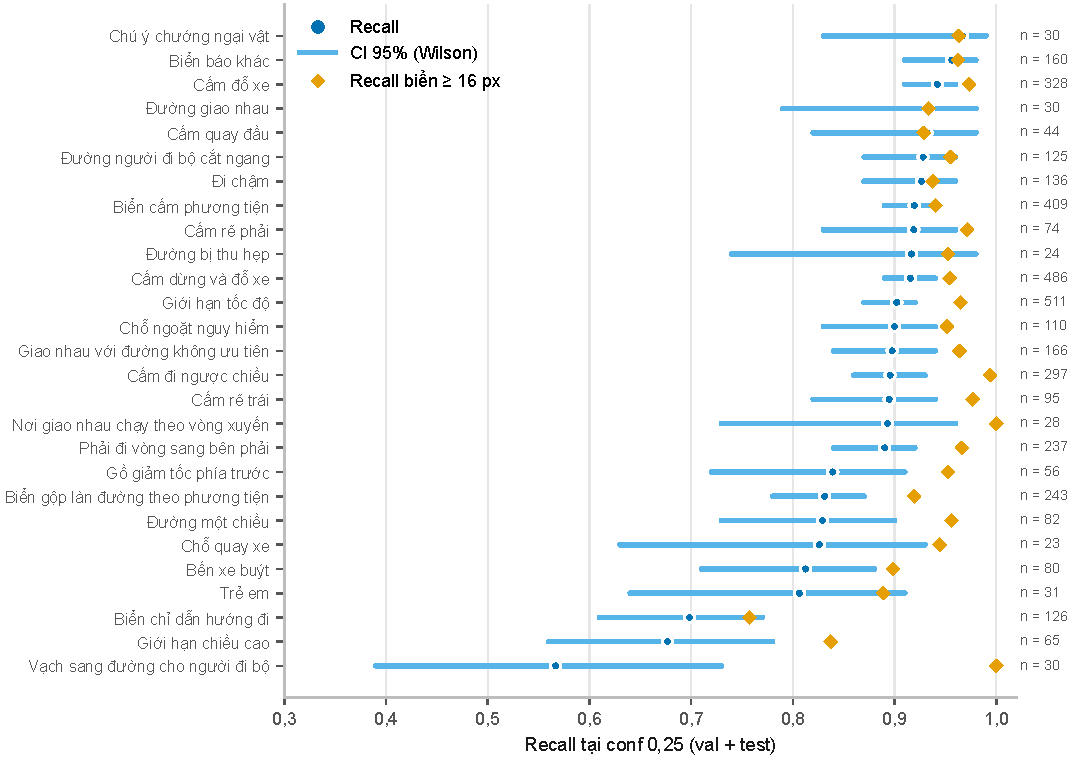
\includegraphics[width=.94\textwidth]{figures/ch3_theo_lop.pdf}
\caption{Recall theo lớp của YOLO11s (val + test, ngưỡng $0{,}25$) kèm CI 95\% Wilson}
\label{fig:per_class}
\end{figure}

\subsection{Theo mức tương đồng với tập huấn luyện}
\label{sec:similarity}
Dù dữ liệu được chia theo cụm và không ảnh kiểm thử nào gần trùng ảnh huấn luyện (khoảng cách pHash $\le6$), khoảng một phần ba ảnh kiểm thử vẫn khá giống ảnh huấn luyện (cùng tuyến đường, cùng camera). Hình~\ref{fig:similarity} chia ảnh kiểm thử theo khoảng cách pHash tới ảnh huấn luyện gần nhất. Kết quả giảm rõ khi cảnh càng khác: recall từ 0,978 xuống 0,805 và precision từ 0,942 xuống 0,749. Ngay cả khi chỉ xét biển từ 16~px trở lên, recall vẫn giảm từ 0,978 xuống 0,893, và precision giảm mạnh nhất: cảnh lạ sinh nhiều phát hiện sai trên nền. Kết quả trên nhóm ``khác train'' là ước lượng gần hơn cho ảnh của tuyến đường mới.

\begin{figure}[H]
\centering
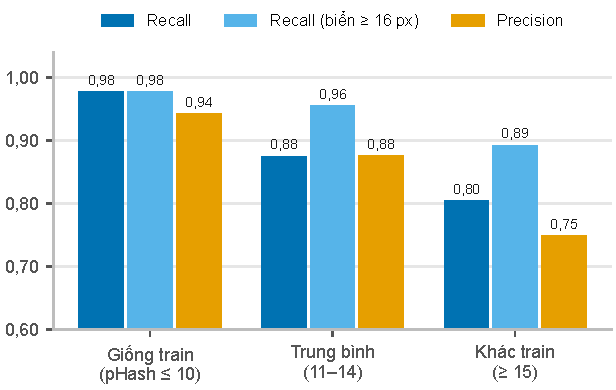
\includegraphics[width=.72\textwidth]{figures/ch3_tuong_dong.pdf}
\caption{Kết quả của YOLO11s theo mức tương đồng của ảnh kiểm thử với tập huấn luyện}
\label{fig:similarity}
\fignote{Số ảnh / số biển: 243 / 667 (giống), 271 / 746 (trung bình), 265 / 604 (khác).}
\end{figure}

\section{Biển nhỏ: độ phân giải suy luận và cắt ô (T3)}
\label{sec:t3}

Vì không thể bổ sung dữ liệu, nhóm thử hai cách tăng recall biển nhỏ mà không cần huấn luyện lại: tăng kích thước ảnh khi suy luận lên 1280 px và cắt ảnh thành các ô 640 px chồng lấn theo kiểu SAHI~\cite{akyon2022sahi}. Kết quả ở Bảng~\ref{tab:t3} và Hình~\ref{fig:t3}.

\begin{table}[H]
\centering
\caption{Ảnh hưởng của cách suy luận đến biển nhỏ (cùng trọng số huấn luyện ở 960 px)}
\label{tab:t3}
\small
\begin{tabularx}{\textwidth}{|>{\raggedright\arraybackslash}X|>{\centering\arraybackslash}p{1.9cm}|>{\centering\arraybackslash}p{1.6cm}|>{\centering\arraybackslash}p{1.6cm}|>{\centering\arraybackslash}p{2.3cm}|>{\centering\arraybackslash}p{1.9cm}|}
\toprule
\textbf{Cách suy luận} & \textbf{Precision} & \textbf{Recall} & \textbf{$F_1$} & \textbf{Recall $<16$ px} & \textbf{ms / ảnh} \\
\midrule
960 px (như khi huấn luyện) & 0,861 & 0,893 & 0,877 & 0,634 & 18,6 \\ \hline
\textbf{1280 px (mặc định)} & \textbf{0,861} & 0,917 & \textbf{0,888} & 0,737 & 21,4 \\ \hline
960 px + cắt ô 640 & 0,749 & \textbf{0,932} & 0,831 & \textbf{0,784} & 46,5 \\
\bottomrule
\end{tabularx}
\tablenote{GPU RTX 4060 Laptop; thời gian chỉ gồm khâu phát hiện.}
\end{table}

\begin{figure}[H]
\centering
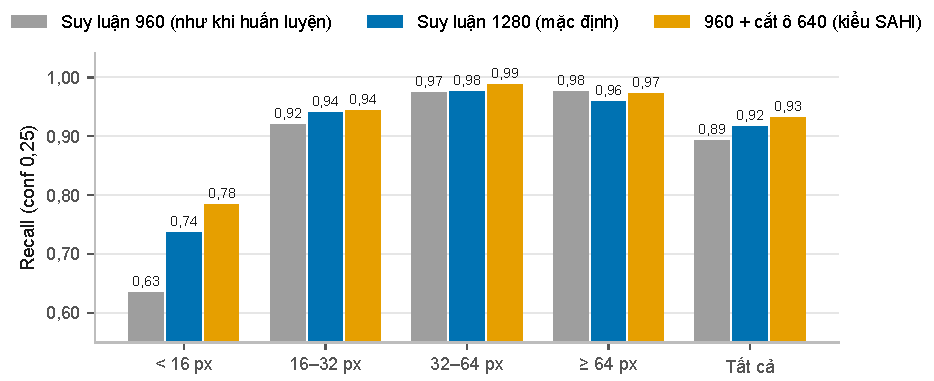
\includegraphics[width=\textwidth]{figures/ch3_t3_kich_thuoc.pdf}
\caption{Recall theo kích thước biển với ba cách suy luận}
\label{fig:t3}
\end{figure}

Suy luận ở 1280 px tăng recall biển dưới 16~px thêm 10,3 điểm (0,634 $\rightarrow$ 0,737) mà precision giữ nguyên và chỉ chậm thêm khoảng 15\%; recall biển từ 64~px giảm nhẹ (0,976 $\rightarrow$ 0,958) vì một số biển lớn bị phóng quá kích thước mô hình đã học. Cắt ô cho recall cao nhất nhưng precision giảm 0,11 do ô cắt làm mất ngữ cảnh và tạo nhiều phát hiện sai ở mép ô, đồng thời chậm 2,5 lần. Nhóm chọn 1280 px làm mặc định và giữ cắt ô làm tuỳ chọn cho ảnh tĩnh độ phân giải cao.

\section{Tăng cường ảnh khi điều kiện xấu (T4, E4)}
\label{sec:t4}

826 ảnh kiểm thử được làm xấu nhân tạo rồi đưa qua YOLO11s (960 px) theo ba chế độ: không xử lý, tăng cường thích nghi của hệ thống (Mục~\ref{sec:enhance}) và luôn áp gamma + CLAHE cho mọi ảnh (đối chứng). Bảng~\ref{tab:t4} cho kết quả kèm CI bootstrap ghép cặp 1\,000 lần theo ảnh.

\begin{table}[H]
\centering
\caption{Recall của YOLO11s khi ảnh bị làm xấu, với ba chế độ tăng cường}
\label{tab:t4}
\small
\begin{tabularx}{\textwidth}{|>{\raggedright\arraybackslash}p{2.6cm}|>{\centering\arraybackslash}p{1.8cm}|>{\centering\arraybackslash}X|>{\centering\arraybackslash}X|}
\toprule
\textbf{Điều kiện} & \textbf{Không xử lý} & \textbf{Thích nghi: \% ảnh xử lý; R; $\Delta$R (CI 95\%)} & \textbf{Luôn gamma + CLAHE: R; $\Delta$R (CI 95\%)} \\
\midrule
Ảnh gốc & 0,893 & 2,8\%; 0,892; $-0{,}001$ ($-0{,}003$; $0{,}000$) & 0,890; $-0{,}003$ ($-0{,}010$; $+0{,}004$) \\ \hline
Tối ($\gamma$ 2,5) & 0,810 & 68,2\%; 0,853; $\mathbf{+0{,}044}$ ($+0{,}032$; $+0{,}056$) & 0,873; $+0{,}063$ ($+0{,}049$; $+0{,}077$) \\ \hline
Rất tối ($\gamma$ 3,5) & 0,686 & 80,5\%; \textbf{0,822}; $\mathbf{+0{,}136}$ ($+0{,}116$; $+0{,}155$) & 0,854; $+0{,}168$ ($+0{,}147$; $+0{,}188$) \\ \hline
Nhiễu ($\sigma$ 15) & 0,799 & 2,8\%; 0,799; $0{,}000$ ($-0{,}001$; $+0{,}001$) & 0,706; $\mathbf{-0{,}093}$ ($-0{,}109$; $-0{,}077$) \\ \hline
Mờ chuyển động & 0,748 & 2,8\%; 0,748; $0{,}000$ ($-0{,}001$; $+0{,}002$) & 0,734; $-0{,}014$ ($-0{,}024$; $-0{,}004$) \\
\bottomrule
\end{tabularx}
\end{table}

\begin{figure}[H]
\centering
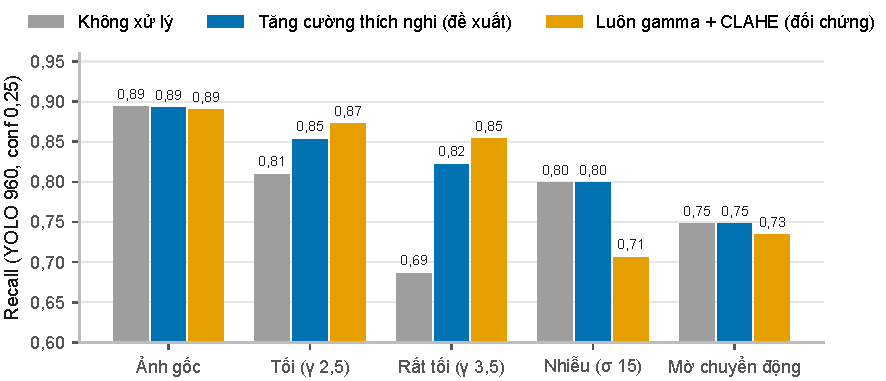
\includegraphics[width=\textwidth]{figures/ch3_t4_tang_cuong.pdf}
\caption{Recall của YOLO11s trên ảnh bị làm xấu với ba chế độ tăng cường}
\label{fig:t4}
\end{figure}

Ba nhận xét rút ra từ Bảng~\ref{tab:t4} và Hình~\ref{fig:t4}:
\begin{enumerate}
 \item \textbf{Tăng cường truyền thống có tác dụng rõ với ảnh tối.} Chế độ thích nghi khôi phục 53\% ($\gamma$ 2,5) và 66\% ($\gamma$ 3,5) phần recall bị mất, có ý nghĩa thống kê, và đạt yêu cầu recall $\ge0{,}80$ trên ảnh rất tối. Precision giảm nhẹ (khoảng 0,02) vì ảnh sáng hơn làm lộ thêm vật thể giống biển.
 \item \textbf{Bước đánh giá chất lượng là cần thiết.} Áp CLAHE cho mọi ảnh làm hại ảnh nhiễu (recall giảm 0,093) và ảnh mờ, vì CLAHE khuếch đại cả nhiễu. Chế độ thích nghi không kích hoạt ở các trường hợp này nên không gây hại, và gần như không chạm vào ảnh tốt (2,8\% ảnh gốc).
 \item \textbf{Hạn chế.} Ngưỡng tối $\mu_V<0{,}30$ bỏ sót 20--32\% ảnh đã làm tối, nên chế độ thích nghi kém hơn ``luôn áp'' trên ảnh tối. Phương sai Laplacian không phân biệt được nhiễu Gauss với chi tiết thật như tán lá, nên lọc song phương chưa được kích hoạt trong thí nghiệm này; chưa có bằng chứng về tác dụng khử nhiễu.
\end{enumerate}

Khi đưa vào hệ thống đầy đủ (E4, suy luận 1280 px, ảnh tối $\gamma$ 2,5), hệ thống đạt precision 0,884, recall 0,866 và $F_1$ 0,875. Hình~\ref{fig:dark} minh hoạ trên một ảnh làm tối $\gamma$ 3,5: sau khi bộ đánh giá chất lượng chọn gamma và CLAHE ($\mu_V=0{,}14$), YOLO11s tìm thêm các biển ở mép phải ảnh mà ảnh tối bỏ sót.

\begin{figure}[H]
\centering
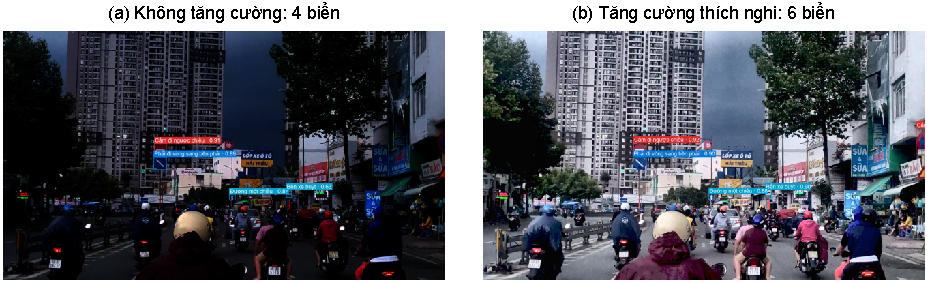
\includegraphics[width=\textwidth]{figures/ch3_anh_toi.pdf}
\caption{Ảnh kiểm thử làm tối ($\gamma$ 3,5) trước và sau tăng cường thích nghi}
\label{fig:dark}
\end{figure}

\section{So sánh đặc trưng thủ công và học sâu (E8)}
\label{sec:e8}

\subsection{Thiết kế so sánh}
Theo cách tách đánh giá của GTSRB và GTSDB~\cite{stallkamp2012gtsrb,houben2013gtsdb}, thí nghiệm E8 so sánh riêng khâu \textit{phân loại} trên cùng 2\,017 biển kiểm thử. Các phương pháp truyền thống (HOG + SVM, HOG + màu + SVM, SIFT-BoVW + SVM) được huấn luyện trên 9\,449 vùng biển của tập huấn luyện, chọn $C$ trên 2\,009 vùng của tập xác thực và được \textit{cho sẵn vị trí biển} (vùng cắt từ nhãn thật, nới 10\%). YOLO11s phải tự tìm biển: lớp của nó là lớp của dự đoán có điểm cao nhất với IoU $\ge0{,}5$; nếu không có thì tính là sai. Vì phương pháp truyền thống có lợi thế được cho vị trí, phép so sánh công bằng là trên 1\,956 biển mà YOLO tìm thấy (cùng tập mẫu cho mọi phương pháp).

\subsection{Kết quả}

\begin{table}[H]
\centering
\caption{Phân loại biển: đặc trưng thủ công + SVM so với YOLO11s (tập kiểm thử)}
\label{tab:e8}
\small
\begin{tabularx}{\textwidth}{|>{\raggedright\arraybackslash}X|>{\centering\arraybackslash}p{3.0cm}|>{\centering\arraybackslash}p{1.6cm}|>{\centering\arraybackslash}p{2.5cm}|>{\centering\arraybackslash}p{1.6cm}|}
\toprule
\textbf{Phương pháp} & \textbf{Accuracy (CI 95\%)} & \textbf{Macro-$F_1$} & \textbf{Acc.\ trên biển YOLO tìm thấy} & \textbf{ms / vùng} \\
\midrule
SIFT-BoVW + SVM & 0,711 (0,691--0,730) & 0,662 & 0,724 & 2,7 \\ \hline
HOG + SVM & 0,888 (0,874--0,901) & 0,852 & 0,901 & 1,6 \\ \hline
HOG + màu + SVM & 0,910 (0,897--0,922) & 0,872 & 0,920 & 2,0 \\ \hline
\textbf{YOLO11s} & \textbf{0,924} (0,912--0,935) & \textbf{0,917} & \textbf{0,953} & 22$^{*}$ \\
\bottomrule
\end{tabularx}
\tablenote{$^{*}$ms trên mỗi ảnh, gồm cả tìm biển (GPU); các phương pháp truyền thống chạy trên CPU.}
\end{table}

\begin{figure}[H]
\centering
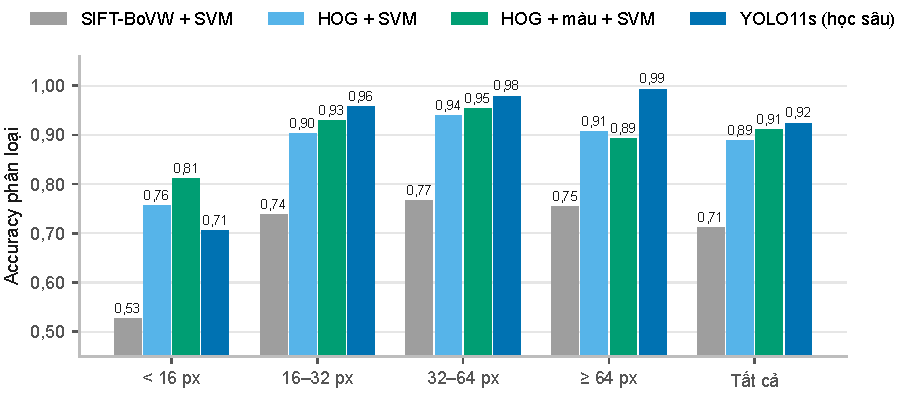
\includegraphics[width=\textwidth]{figures/ch3_e8_phan_loai.pdf}
\caption{Accuracy phân loại theo kích thước biển của bốn phương pháp}
\label{fig:e8}
\fignote{Phương pháp truyền thống được cho sẵn vị trí biển; YOLO11s bị tính sai cả khi bỏ sót biển.}
\end{figure}

\begin{figure}[H]
\centering
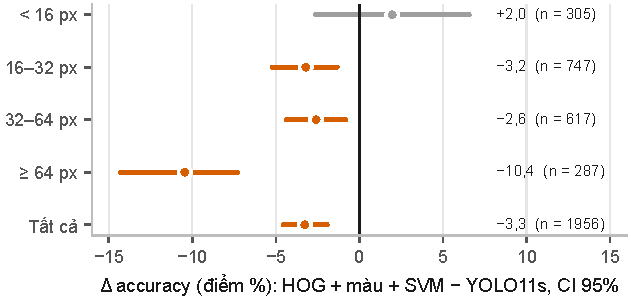
\includegraphics[width=.8\textwidth]{figures/ch3_e8_ghep_cap.pdf}
\caption{Chênh lệch accuracy ghép cặp giữa HOG + màu + SVM và YOLO11s trên các biển YOLO tìm thấy (bootstrap 2\,000 lần)}
\label{fig:e8_paired}
\fignote{Màu đỏ: CI 95\% không chứa 0 (khác biệt có ý nghĩa); màu xám: không khác biệt.}
\end{figure}

Từ Bảng~\ref{tab:e8}, Hình~\ref{fig:e8} và Hình~\ref{fig:e8_paired}:
\begin{enumerate}
 \item \textbf{Đặc trưng thủ công cạnh tranh được ở khâu phân loại.} HOG + màu + SVM chỉ kém YOLO11s 1,4 điểm accuracy tổng. Thêm histogram màu HSV vào HOG tăng 2,2 điểm: màu là thông tin quy chuẩn mà HOG trên ảnh xám bỏ qua. Kết quả 91,0\% cùng mức với HOG-SVM trên GTSRB (89,65--91,25\%~\cite{vieira2025hogsvm}), dù không so sánh trực tiếp được vì khác dữ liệu.
 \item \textbf{Với biển nhỏ, điểm yếu của YOLO là tìm biển, không phải phân loại.} YOLO bỏ sót 15,5\% số biển dưới 16~px. Trên các biển nhỏ mà YOLO tìm thấy, hai phương pháp ngang nhau: chênh lệch $+2{,}0$ điểm, CI 95\% từ $-2{,}6$ đến $+6{,}6$. Khi được cho vị trí, HOG + màu đúng 81,2\% số biển nhỏ, so với 70,6\% của YOLO (tính cả biển bỏ sót).
 \item \textbf{Biển lớn là nơi đặc trưng thủ công thua rõ nhất} ($-10{,}4$ điểm, CI từ $-14{,}3$ đến $-7{,}3$). Thu vùng về $32\times32$ làm mất chi tiết của biển chỉ dẫn và biển có chữ, trong khi CNN học đặc trưng ở nhiều tỉ lệ.
 \item \textbf{SIFT không phù hợp với biển báo.} SIFT-BoVW kém HOG 17,7 điểm. Số điểm SIFT trung vị chỉ là 1 với biển dưới 16~px (93\% số biển có dưới 5 điểm), 8 với biển 16--32~px và 74 với biển từ 64~px. Biển báo là vùng phẳng với ký hiệu đơn giản, ít điểm góc và kết cấu, nên điểm khoá chủ yếu nằm trên viền tròn chung của nhiều lớp.
 \item \textbf{Đặc trưng thủ công rẻ} (1,6--2,7 ms mỗi vùng trên CPU) nhưng cần một bước định vị riêng --- chính là phần YOLO làm tốt.
\end{enumerate}

\subsection{So sánh hai hệ thống trên cùng ảnh}
Khác với E8, Hình~\ref{fig:qualitative} so sánh \textit{toàn bộ} hai hệ thống, gồm cả bước định vị: YOLO11s và pipeline đối chứng (màu + hình dạng + HOG + SVM). Trên ảnh có 16 biển được gán nhãn (hàng đầu), YOLO11s trả 22 phát hiện, còn pipeline truyền thống chỉ trả 8; số phát hiện của YOLO lớn hơn số nhãn vì có cả biển ở xa không được gán nhãn và một số phát hiện trùng. Pipeline truyền thống gộp các biển cùng màu đứng sát nhau thành một vùng, bỏ sót biển chỉ dẫn nhiều màu và biển rất nhỏ, và báo nhầm trên vùng đỏ như áo người đi xe máy (hàng giữa). Khi YOLO11s cung cấp vị trí, HOG + màu + SVM đồng ý với YOLO ở 14/22 biển của ảnh hàng đầu. Như vậy, trong hệ thống truyền thống, bước định vị bằng màu--hình dạng mới là nút thắt, không phải bước phân loại.

\begin{figure}[H]
\centering
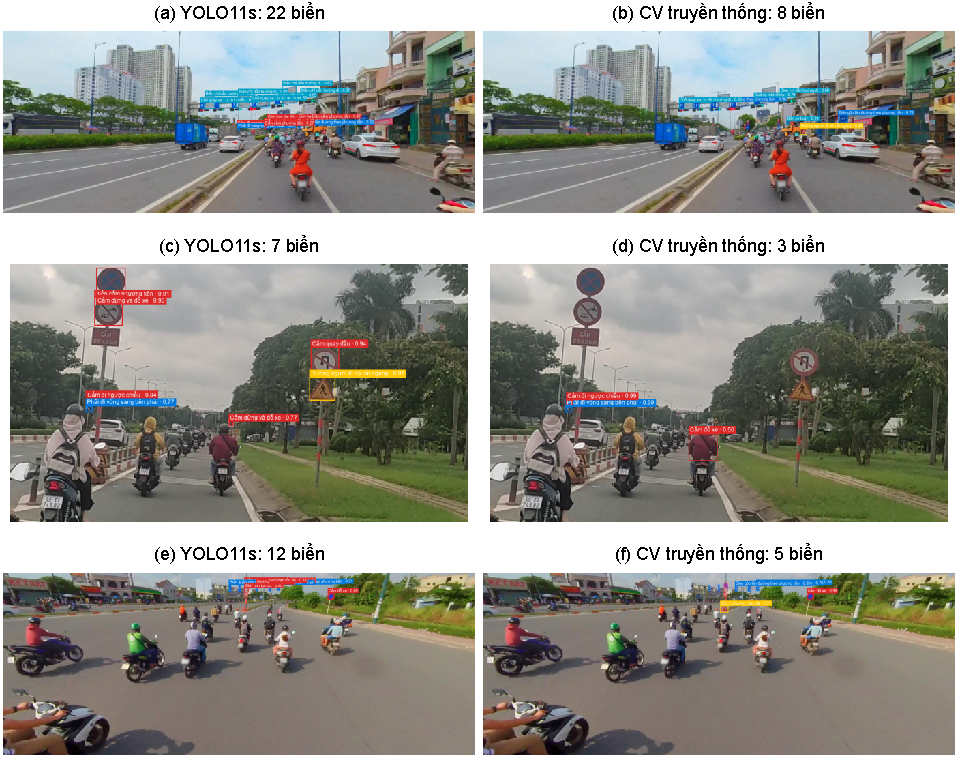
\includegraphics[width=\textwidth]{figures/ch3_dinh_tinh.pdf}
\caption{Kết quả của YOLO11s (trái) và pipeline CV truyền thống (phải) trên ba ảnh của tập kiểm thử}
\label{fig:qualitative}
\fignote{Cùng ảnh đầu vào, cùng khâu tăng cường thích nghi; số biển là số phát hiện mà mỗi hệ thống trả về.}
\end{figure}

\section{Bộ xác minh bằng đặc trưng thủ công (T0, T1)}
\label{sec:t1}

Thí nghiệm T0 cho thấy dư địa lý thuyết của bộ xác minh là lớn: 68--71\% phát hiện sai của YOLO11s là vùng nền (phần còn lại là sai lớp 21--25\% và định vị kém 4--8\%, tuỳ tập và ngưỡng) --- đúng loại lỗi mà màu và hình dạng có thể nhận ra. Tuy nhiên, chính điểm tin cậy của YOLO đã phân biệt phát hiện đúng và sai rất tốt (AUC 0,941). Thí nghiệm T1 học LightGBM trên phát hiện của tập xác thực với các tập đặc trưng khác nhau và đánh giá trên tập kiểm thử (Bảng~\ref{tab:t1}).

\begin{table}[H]
\centering
\caption{Ablation tập đặc trưng của bộ xác minh (học trên val, đánh giá trên test)}
\label{tab:t1}
\small
\begin{tabularx}{\textwidth}{|>{\raggedright\arraybackslash}X|>{\centering\arraybackslash}p{1.4cm}|>{\centering\arraybackslash}p{2.2cm}|>{\centering\arraybackslash}p{3.3cm}|}
\toprule
\textbf{Tập đặc trưng} & \textbf{AUC} & \textbf{P cùng recall (R 0,893)} & \textbf{P / R với ngưỡng chọn trên val} \\
\midrule
Điểm YOLO (không xác minh) & \textbf{0,941} & 0,864 & 0,864 / 0,893 \\ \hline
Ngữ cảnh YOLO (điểm, lớp, kích thước, vị trí) & 0,929 & 0,864 & 0,886 / 0,879 \\ \hline
\quad + màu HSV & 0,933 & 0,863 & 0,880 / 0,881 \\ \hline
\quad + màu + hình học + Hu & 0,935 & 0,859 & 0,875 / 0,888 \\ \hline
\quad + màu + hình học + Hu + HOG & 0,935 & \textbf{0,876} & 0,873 / 0,895 \\ \hline
Đầy đủ (thêm độ nét, độ sáng) & 0,934 & 0,866 & 0,878 / 0,891 \\ \hline
Chỉ đặc trưng thủ công (không có điểm YOLO) & 0,856 & 0,832 & 0,842 / 0,888 \\
\bottomrule
\end{tabularx}
\end{table}

Ở cùng recall với YOLO, chênh lệch precision của bộ xác minh đầy đủ là $+0{,}005$ với CI 95\% từ $-0{,}012$ đến $+0{,}022$, tức không có ý nghĩa thống kê; mục tiêu ban đầu là precision $\ge0{,}90$ không đạt. Đặc trưng thủ công có tín hiệu (AUC 0,856 khi đứng một mình, xa mức ngẫu nhiên 0,5) nhưng trùng lặp với thông tin mạng tích chập đã học: biển được YOLO cho điểm cao hầu như luôn có màu và hình dạng đúng. Bộ xác minh còn thiếu mẫu âm để học (chỉ khoảng 500 phát hiện sai trên tập xác thực so với 1\,828 phát hiện đúng), và không thể thêm ảnh nền khó vì dữ liệu đã đóng băng. Vì vậy, bộ xác minh được giữ như một kết quả ablation trung thực và tắt mặc định trong hệ thống.

\section{Hệ thống đầy đủ (E1) và đóng góp của từng khâu (E2)}
\label{sec:e1}

Cấu hình mặc định sau các thí nghiệm là: tăng cường thích nghi bật, YOLO11s suy luận 1280 px, bộ xác minh tắt, đọc chữ bật. Bảng~\ref{tab:e1} cho kết quả của cấu hình này.

\begin{table}[H]
\centering
\caption{Kết quả của hệ thống với cấu hình mặc định (E1)}
\label{tab:e1}
\small
\begin{tabularx}{\textwidth}{|>{\raggedright\arraybackslash}X|>{\centering\arraybackslash}p{1.1cm}|>{\centering\arraybackslash}p{1.1cm}|>{\centering\arraybackslash}p{1.1cm}|>{\centering\arraybackslash}p{1.2cm}|>{\centering\arraybackslash}p{1.2cm}|>{\centering\arraybackslash}p{1.2cm}|>{\centering\arraybackslash}p{1.2cm}|>{\centering\arraybackslash}p{1.3cm}|}
\toprule
\textbf{Tập} & \textbf{P} & \textbf{R} & \textbf{$F_1$} & \textbf{R $<16$} & \textbf{R 16--32} & \textbf{R 32--64} & \textbf{R $\ge64$} & \textbf{ms/ảnh} \\
\midrule
Test & 0,862 & \textbf{0,917} & \textbf{0,889} & \textbf{0,734} & 0,941 & 0,976 & 0,958 & 22,5 \\ \hline
Test làm tối ($\gamma$ 2,5) & 0,884 & 0,866 & 0,875 & 0,662 & 0,860 & 0,948 & 0,958 & 34,8 \\
\bottomrule
\end{tabularx}
\tablenote{GPU RTX 4060 Laptop; thời gian gồm đánh giá chất lượng, tăng cường (khi cần) và phát hiện.}
\end{table}

So với YOLO11s ở 960 px không tăng cường, recall tăng từ 0,893 lên 0,917 và recall biển dưới 16~px từ 0,634 lên 0,734 (đạt mục tiêu $\ge0{,}70$), precision giữ nguyên. Bảng~\ref{tab:e2} là thí nghiệm ablation bật lần lượt từng khâu, đo ở 960 px trước khi đổi mặc định sang 1280 px; theo vết không áp dụng cho ảnh tĩnh nên không có hàng riêng.

\begin{table}[H]
\centering
\caption{Ablation: đóng góp của từng khâu (YOLO 960 px)}
\label{tab:e2}
\small
\begin{tabularx}{\textwidth}{|>{\raggedright\arraybackslash}X|>{\centering\arraybackslash}p{1.25cm}|>{\centering\arraybackslash}p{1.25cm}|>{\centering\arraybackslash}p{1.25cm}|>{\centering\arraybackslash}p{1.3cm}|>{\centering\arraybackslash}p{1.25cm}|>{\centering\arraybackslash}p{1.25cm}|>{\centering\arraybackslash}p{1.25cm}|}
\toprule
\multirow{2}{*}{\textbf{Cấu hình}} & \multicolumn{4}{c|}{\textbf{Test gốc}} & \multicolumn{3}{c|}{\textbf{Test làm tối ($\gamma$ 2,5)}} \\ \cline{2-8}
 & \textbf{P} & \textbf{R} & \textbf{$F_1$} & \textbf{R $<16$} & \textbf{P} & \textbf{R} & \textbf{$F_1$} \\
\midrule
YOLO11s & 0,861 & \textbf{0,893} & 0,877 & \textbf{0,634} & 0,905 & 0,813 & 0,856 \\ \hline
+ tăng cường thích nghi [CV] & 0,860 & \textbf{0,893} & 0,876 & \textbf{0,634} & 0,885 & \textbf{0,854} & 0,869 \\ \hline
+ bộ xác minh [CV + DL] & \textbf{0,946} & 0,841 & \textbf{0,891} & 0,526 & \textbf{0,960} & 0,796 & \textbf{0,871} \\
\bottomrule
\end{tabularx}
\end{table}

Tăng cường thích nghi không thay đổi kết quả trên ảnh thường (chỉ kích hoạt ở khoảng 3\% ảnh) và tăng recall 0,041 trên ảnh tối, khớp với T4. Bộ xác minh tăng precision 0,085 nhưng giảm recall 0,052, riêng biển dưới 16~px giảm 0,108; đây là sự dịch chuyển điểm vận hành, không phải cải thiện thật (T1 cho thấy ở cùng recall nó không hơn điểm YOLO). Bộ xác minh có thể bật lại trên giao diện khi người dùng ưu tiên ít báo nhầm hơn là tìm đủ biển.

Lưu ý: mAP tính trên \textit{đầu ra} của hệ thống (đã cắt ở ngưỡng $0{,}25$) là 0,869 (mAP@50) và 0,667 (mAP@50:95), thấp hơn mAP của mô hình ở Bảng~\ref{tab:baseline} vì đường precision--recall bị cắt ở ngưỡng hiển thị. Giá trị này chỉ dùng để so giữa các cấu hình, không dùng để so với mAP của các công trình khác.

\section{Đọc số và chữ}
\label{sec:ocr_result}
Do không có nhãn chữ, khả năng đọc chỉ được đánh giá định tính. Trên ảnh kiểm thử, hệ thống đọc đúng ``40 km/h'' và ``60 km/h'' trên biển giới hạn tốc độ và ``2,0 m'' trên biển giới hạn chiều cao; Hình~\ref{fig:system_pipeline} có một ví dụ vùng số được cắt và đọc. Chữ trên biển nhỏ thường bị loại vì độ tin cậy của VietOCR dưới 0,75: ngưỡng này được đặt để tránh trả về chuỗi rác, đổi lại hệ thống để trống nội dung thay vì đoán. Đo định lượng bằng CER và tỉ lệ khớp hoàn toàn cần một tập nhãn chữ riêng --- đây là việc cần làm khi có thể bổ sung dữ liệu.

\section{Tốc độ và triển khai}
\label{sec:speed}

Bảng~\ref{tab:speed} tổng hợp các phép đo tốc độ.

\begin{table}[H]
\centering
\caption{Tốc độ của hệ thống}
\label{tab:speed}
\small
\begin{tabularx}{\textwidth}{|>{\raggedright\arraybackslash}X|>{\centering\arraybackslash}p{4.6cm}|}
\toprule
\textbf{Phép đo} & \textbf{Kết quả} \\
\midrule
Khâu phát hiện, 960 px, FP16, GPU RTX 4060 Laptop & 18,3 ms (54,6 FPS) \\ \hline
Đánh giá chất lượng + tăng cường + phát hiện, 1280 px, cùng GPU & 22,5 ms / ảnh \\ \hline
Ảnh tĩnh qua API trong Docker CPU, gồm đọc chữ & 0,9--1,6 s / ảnh \\ \hline
Pipeline CV truyền thống trên CPU, các ảnh mẫu & 50--225 ms / ảnh \\ \hline
Webcam qua WebSocket, CPU, 960 px & 9,3 FPS \\ \hline
Webcam qua WebSocket, Docker CPU, 1280 px & 3,5 FPS \\ \hline
Xử lý video nền 30 khung hình (Docker CPU) & 10 s \\ \hline
Khởi động API, nạp 4 mô hình, không cần mạng & 11 s \\
\bottomrule
\end{tabularx}
\end{table}

Khâu phát hiện đủ nhanh cho thời gian thực trên GPU tầm trung, và ảnh tĩnh qua API trên CPU đạt yêu cầu dưới 3 giây kể cả đọc chữ. Trên CPU, luồng webcam chỉ đạt 3,5--9,3 FPS; webcam thời gian thực cần chạy với GPU, phép đo này chưa được thực hiện qua giao diện web. Thời gian của pipeline truyền thống phụ thuộc số ứng viên vì SVM nhân RBF phải chạy trên từng vùng.

\section{Chương trình demo và giao diện}
\label{sec:demo}

Nhóm xây dựng ứng dụng web để trình diễn và kiểm tra trực tiếp hệ thống. Phần máy chủ là FastAPI dùng lại đúng mã nguồn của pipeline; phần giao diện là React; toàn bộ được đóng gói bằng Docker Compose với hai cấu hình CPU và GPU, chạy được khi không có mạng. Bảng~\ref{tab:demo_pages} tóm tắt các trang chức năng.

\begin{table}[H]
\centering
\caption{Các trang chức năng của ứng dụng web}
\label{tab:demo_pages}
\small
\begin{tabularx}{\textwidth}{|>{\raggedright\arraybackslash}p{3.4cm}|X|}
\toprule
\textbf{Trang} & \textbf{Chức năng chính} \\
\midrule
Mô tả dữ liệu & Thống kê chia tập, 27 lớp, nhóm biển, kích thước, số biển trên ảnh, bản đồ nhiệt vị trí, độ phân giải, kết quả kiểm tra dữ liệu \\ \hline
Pipeline hệ thống & Sơ đồ tương tác của hai hệ thống; chạy một ảnh để xem chỉ số chất lượng, ảnh tăng cường, kết quả YOLO, vùng số và kết quả cuối \\ \hline
Demo học sâu & Chọn ảnh mẫu hoặc tải ảnh; bật/tắt từng khâu (tăng cường, xác minh, cắt ô), đổi kích thước suy luận, mô phỏng ảnh tối, nhiễu, mờ; so sánh trước/sau; lịch sử các lần chạy; xuất JSON và ảnh \\ \hline
Demo CV truyền thống & Từng bước: mặt nạ HSV, vùng ứng viên, kết quả; ảnh HOG, điểm SIFT và lớp SVM của từng ứng viên \\ \hline
So sánh CV -- DL & Chạy hai hệ thống trên cùng ảnh; bảng phân loại của HOG + màu + SVM trên từng biển YOLO tìm thấy; biểu đồ E8 và T4 \\ \hline
Kết quả thực nghiệm & Đường cong huấn luyện, CI 95\%, E1, E2, T3, kết quả theo lớp, theo mức tương đồng, sổ đăng ký thí nghiệm \\ \hline
Video, Webcam, Thư viện biển & Xử lý video nền có theo vết; webcam qua WebSocket; tra cứu 27 lớp theo QCVN \\
\bottomrule
\end{tabularx}
\end{table}

Hình~\ref{fig:web_pipeline} là trang Pipeline hệ thống khi chạy một ảnh có biển giới hạn tốc độ: sơ đồ hai hệ thống ở trên, bên dưới là chỉ số chất lượng ảnh (độ sáng 0,48, tương phản 0,23, nên không cần tăng cường) và kết quả YOLO11s kèm giá trị đọc được ``40 km/h''.

\begin{figure}[H]
\centering
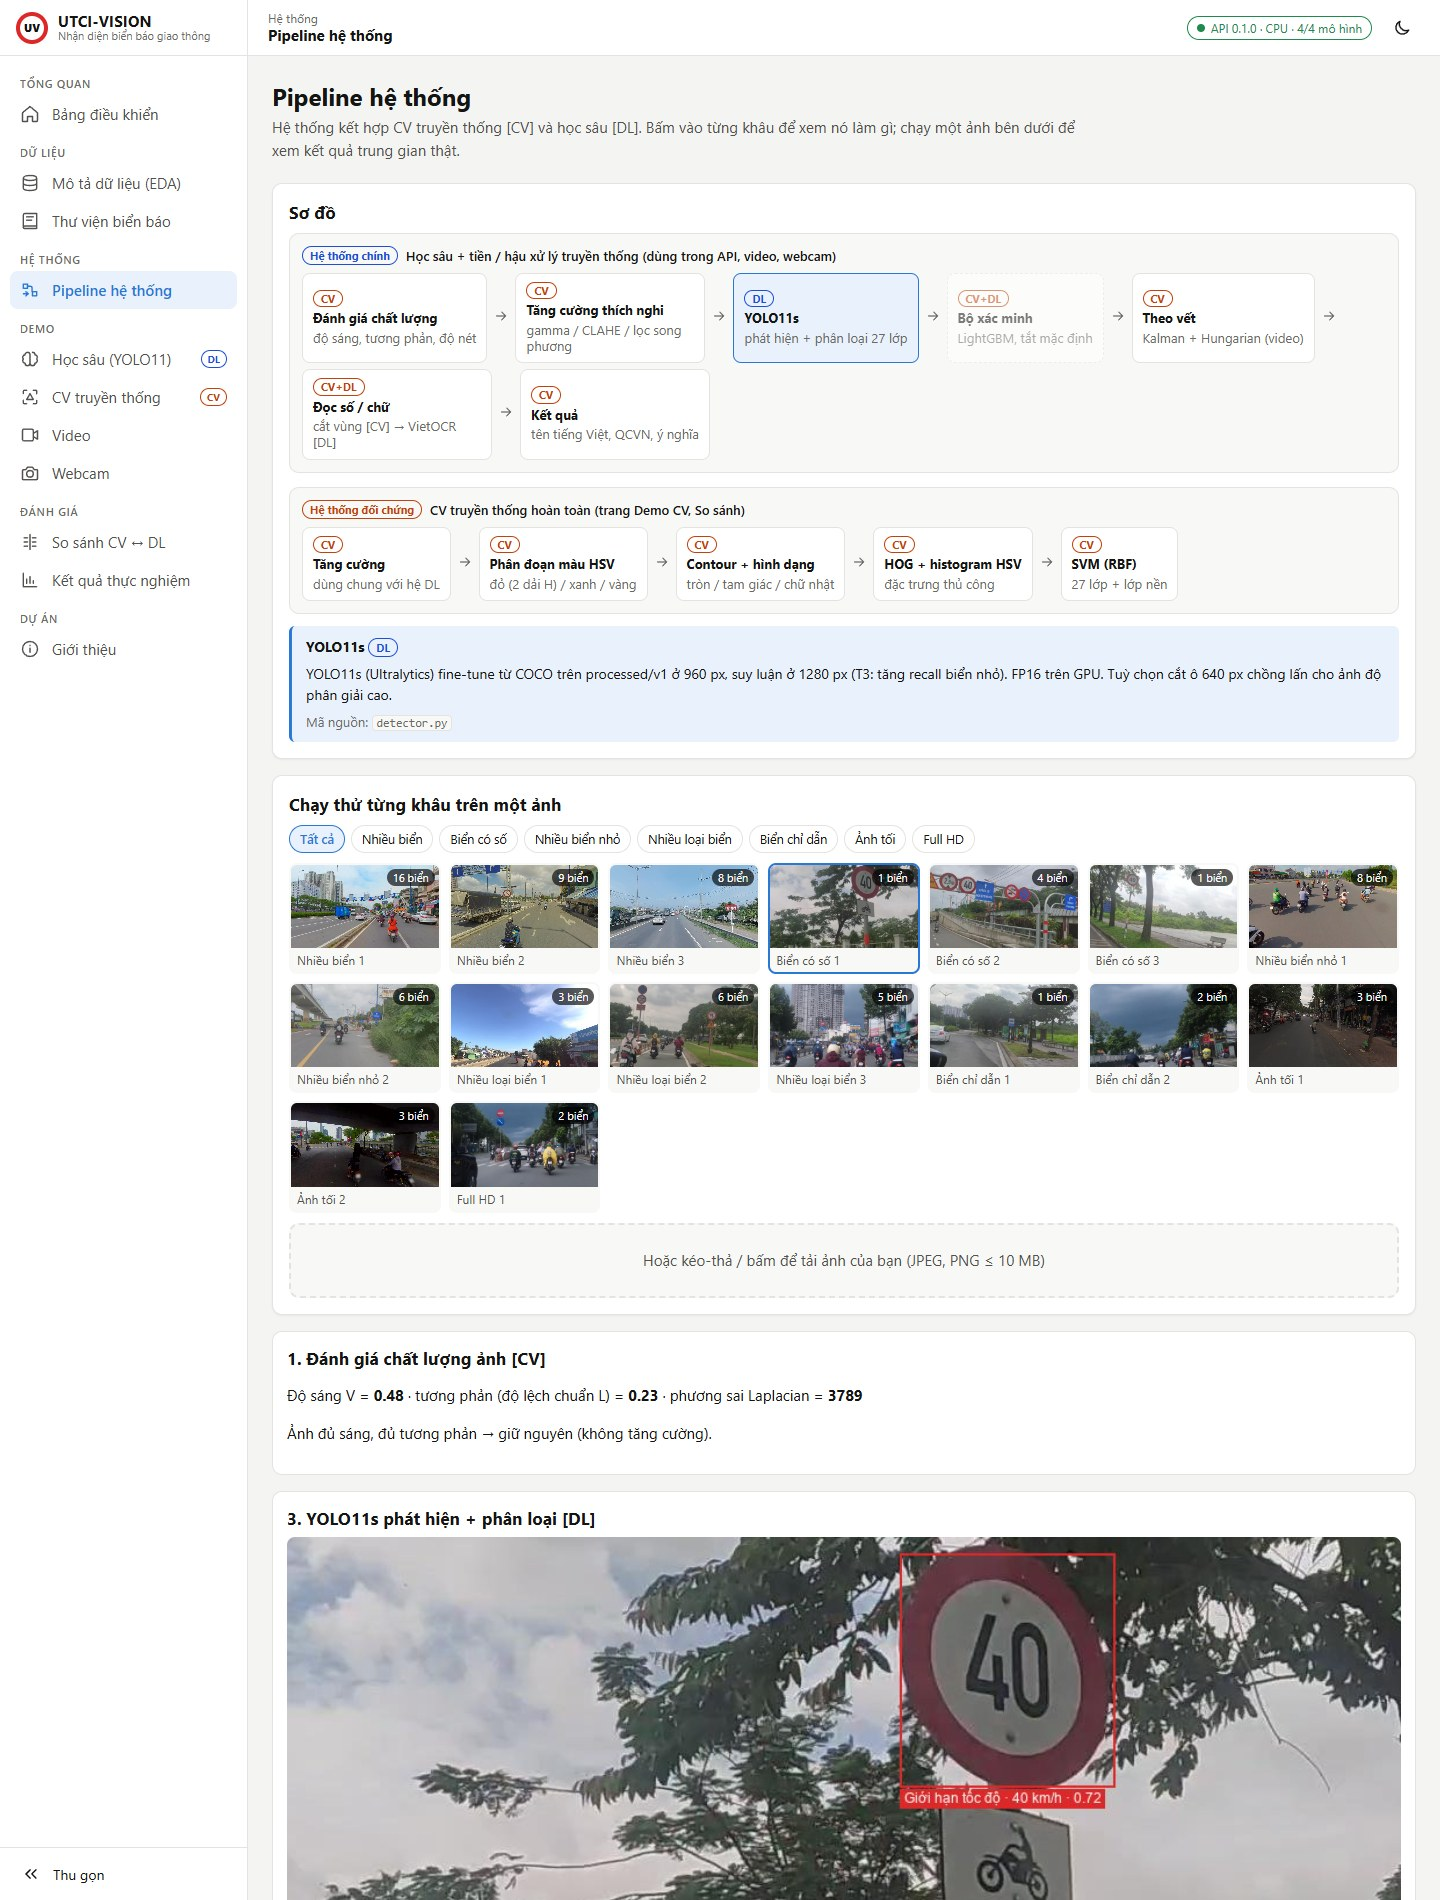
\includegraphics[width=.86\textwidth]{figures/web_pipeline.jpg}
\caption{Trang Pipeline hệ thống: sơ đồ tương tác và kết quả trung gian của từng khâu}
\label{fig:web_pipeline}
\end{figure}

Hình~\ref{fig:web_dl} là trang Demo học sâu với ảnh có nhiều biển nhỏ: người dùng chọn kích thước suy luận, bật/tắt từng khâu và mô phỏng điều kiện xấu; kết quả hiển thị danh sách biển theo nhóm, mã QCVN và thời gian của từng khâu. Đây là cách trình diễn trực tiếp các thí nghiệm T3, T4 và E2.

\begin{figure}[H]
\centering
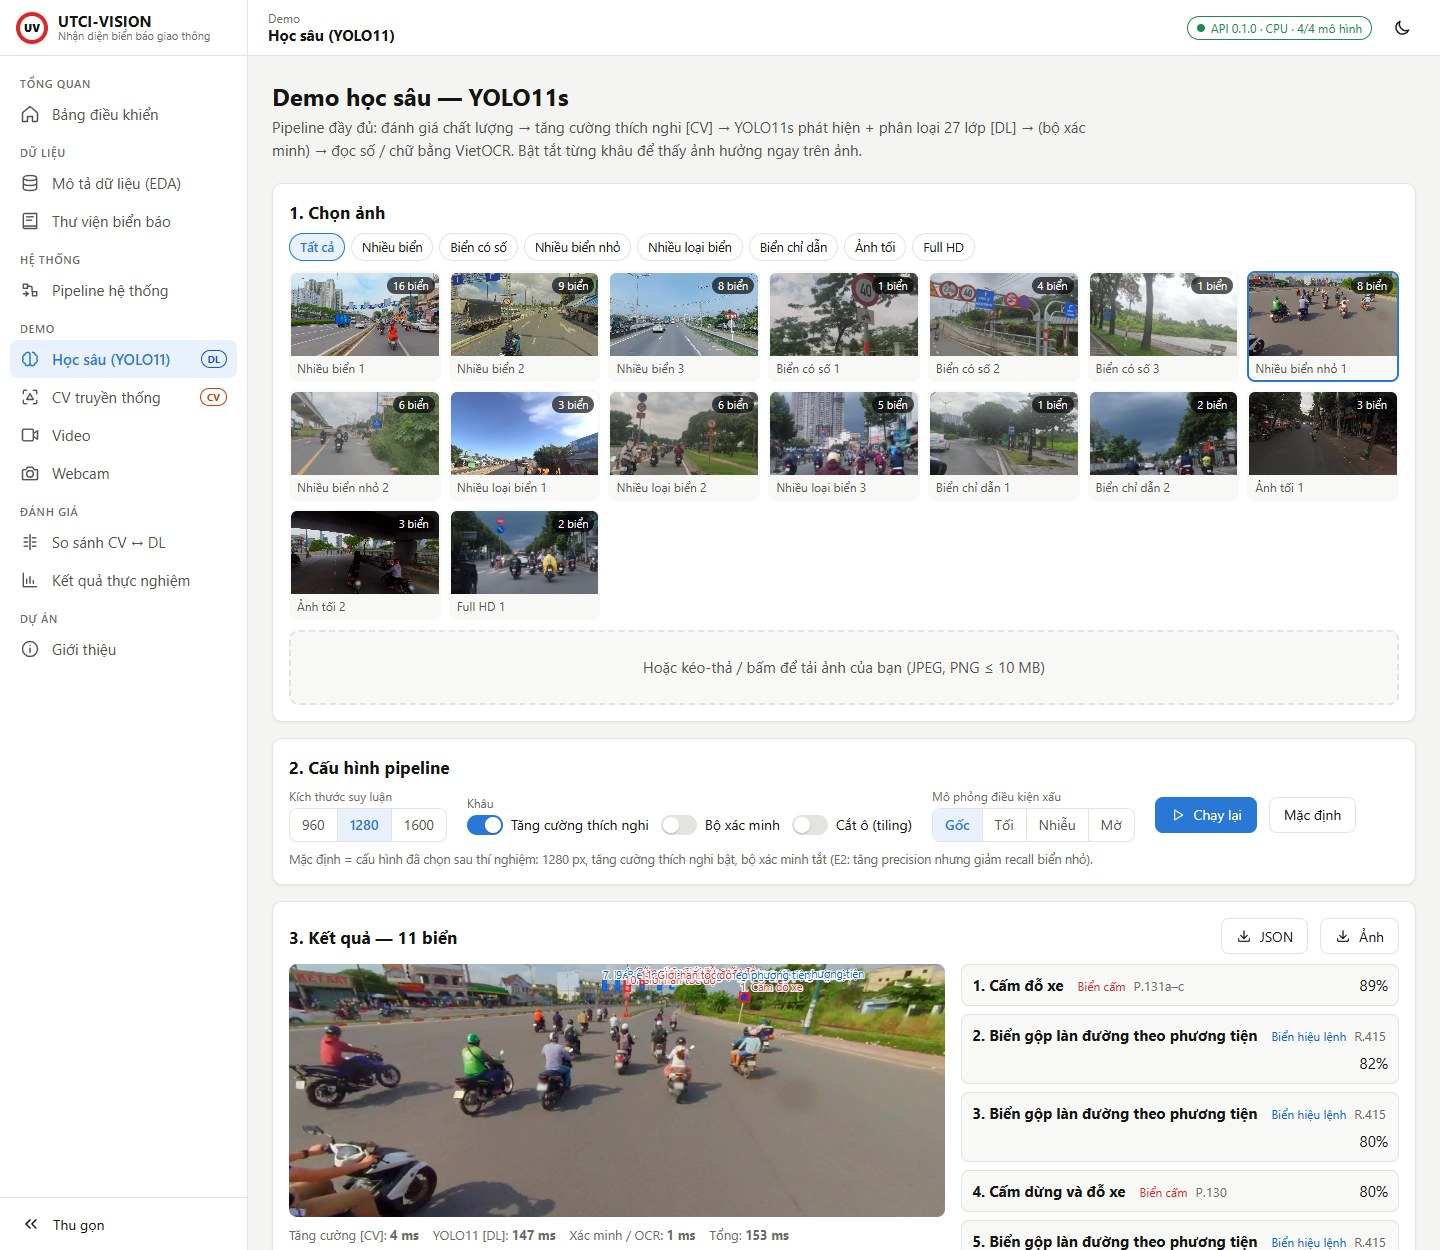
\includegraphics[width=.86\textwidth]{figures/web_dl.jpg}
\caption{Trang Demo học sâu: cấu hình pipeline và kết quả trên ảnh có nhiều biển nhỏ}
\label{fig:web_dl}
\end{figure}

Hình~\ref{fig:web_cv} là trang Demo CV truyền thống, hiển thị lần lượt ảnh đầu vào, mặt nạ màu HSV, vùng ứng viên và kết quả; thời gian từng bước và chỉ số chất lượng ảnh được ghi ngay dưới ảnh. Hình~\ref{fig:web_compare} là trang So sánh, chạy cả hai hệ thống trên cùng ảnh và lập bảng so khớp trên từng biển mà YOLO tìm thấy.

\begin{figure}[H]
\centering
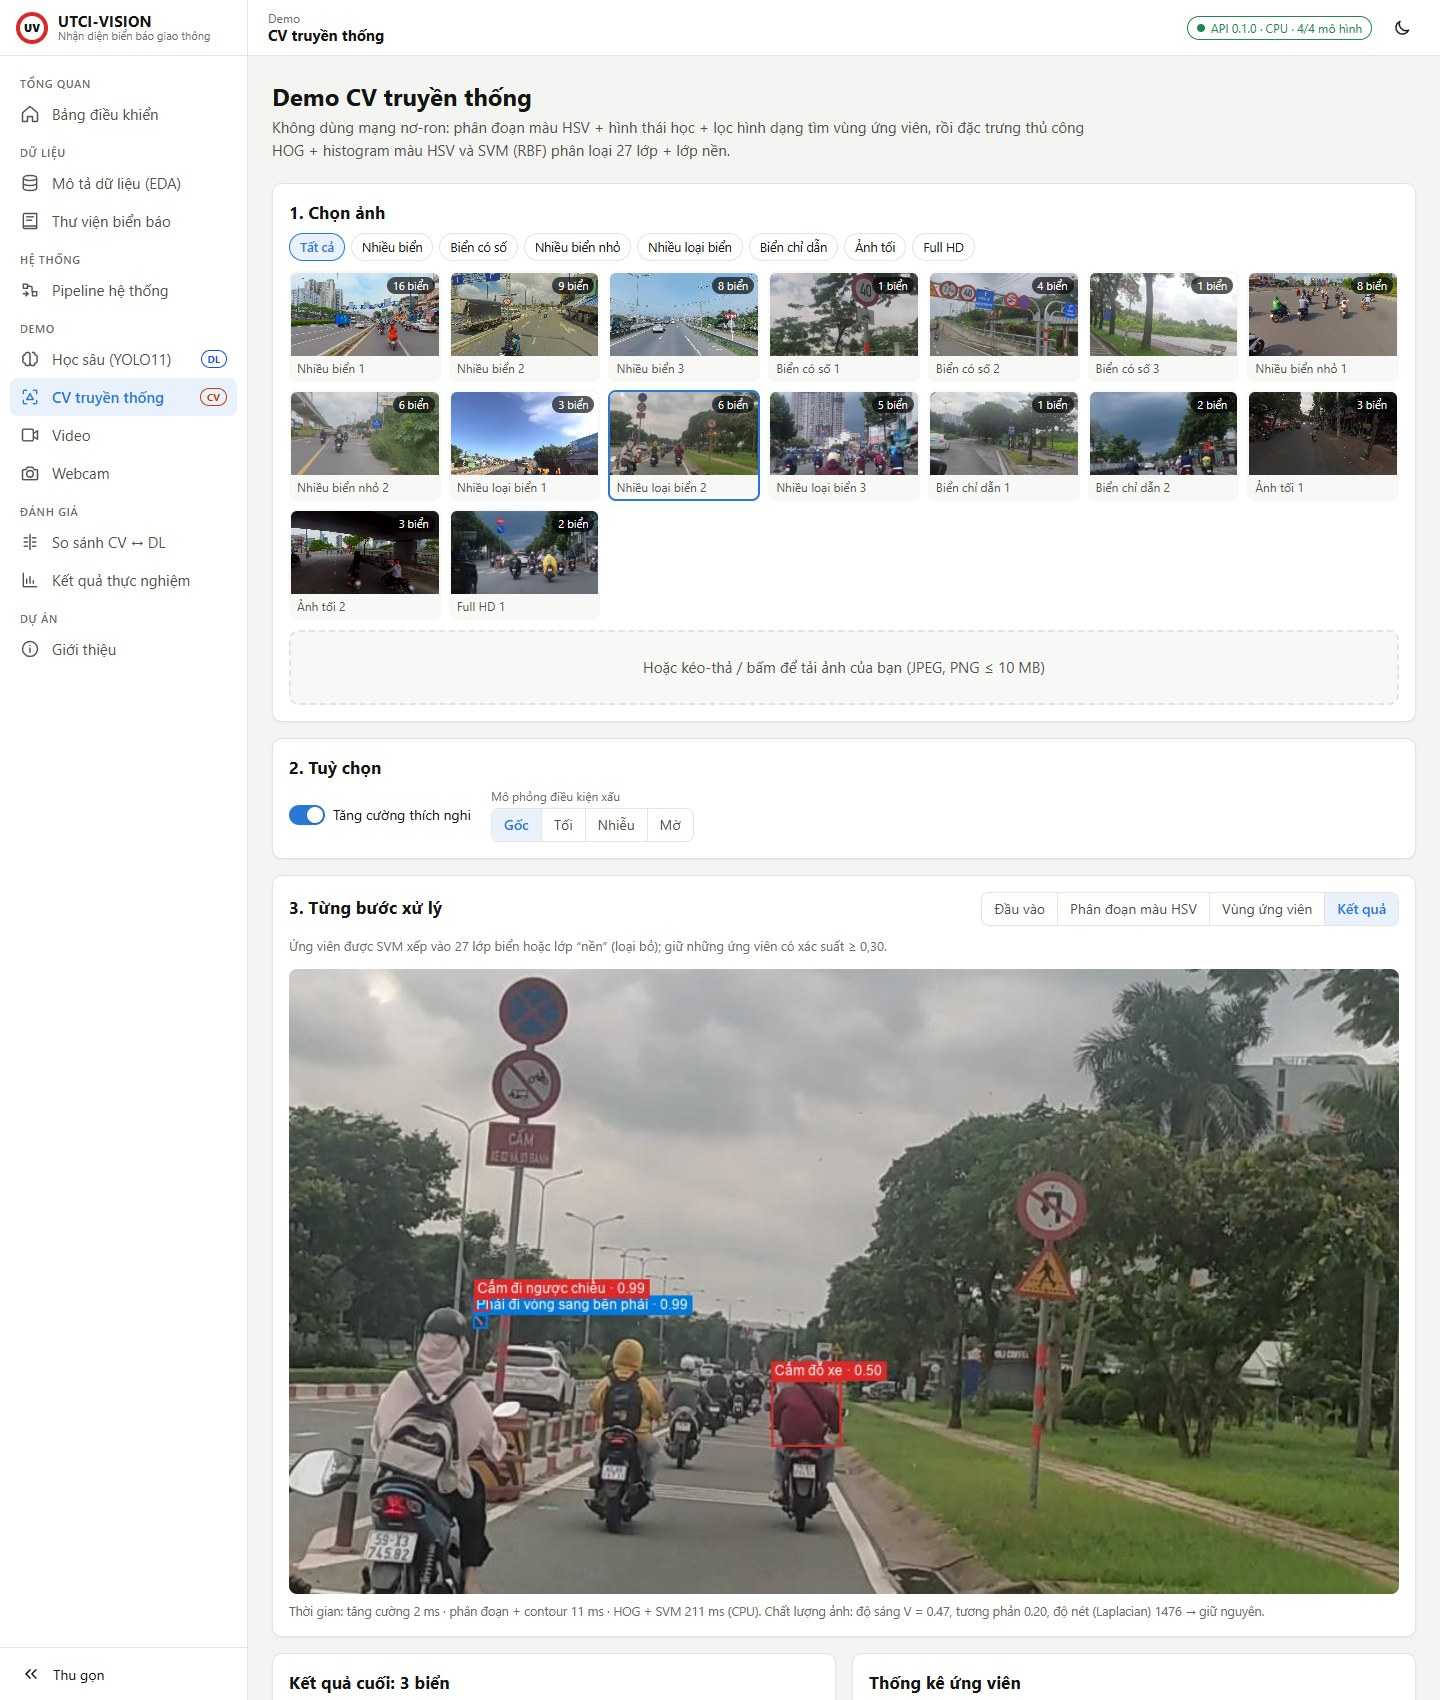
\includegraphics[width=.86\textwidth]{figures/web_cv.jpg}
\caption{Trang Demo CV truyền thống: kết quả của pipeline màu + hình dạng + HOG + SVM}
\label{fig:web_cv}
\end{figure}

\begin{figure}[H]
\centering
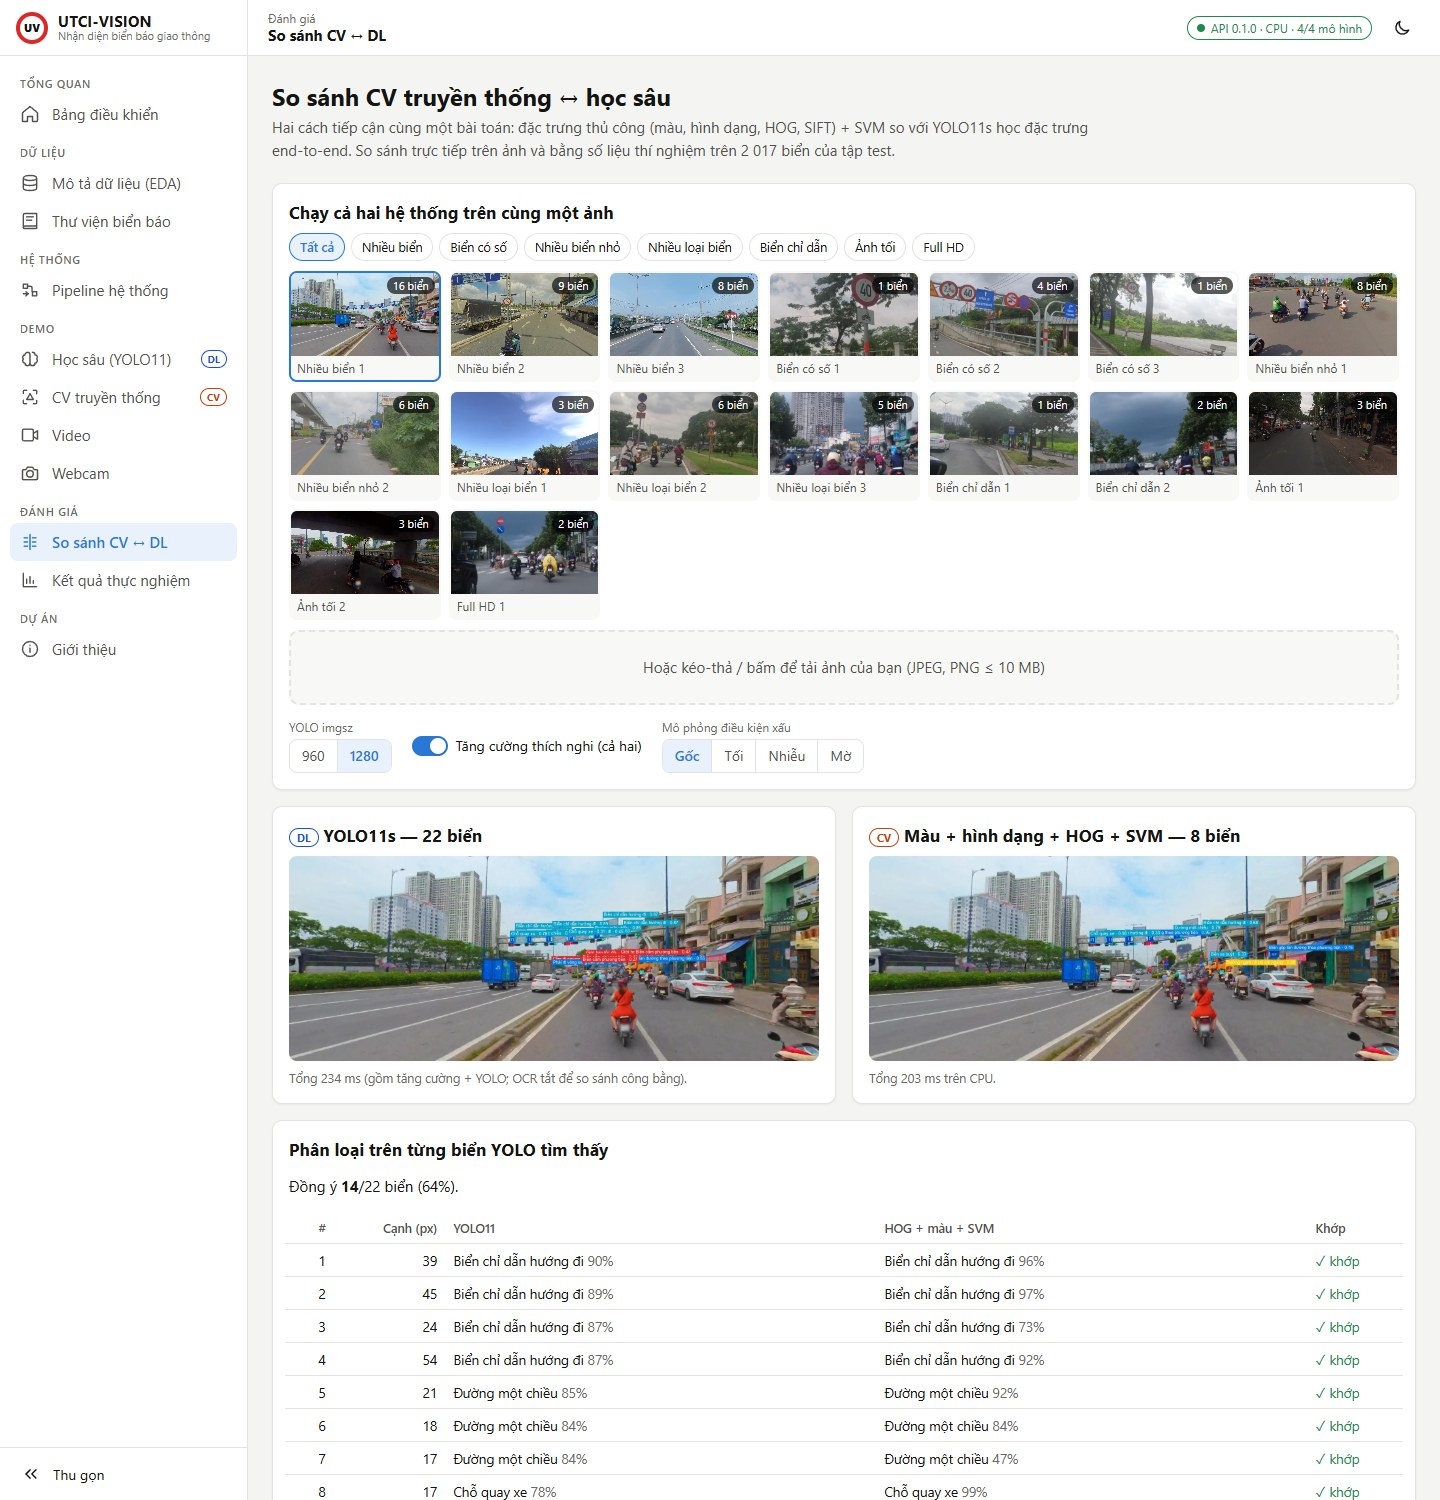
\includegraphics[width=.86\textwidth]{figures/web_compare.jpg}
\caption{Trang So sánh CV -- DL: hai hệ thống trên cùng ảnh và bảng so khớp từng biển}
\label{fig:web_compare}
\end{figure}

\section{Thảo luận}
\label{sec:discussion}

\subsection{Trả lời các câu hỏi đặt ra}
\begin{itemize}
 \item \textbf{Học sâu hay đặc trưng thủ công?} Ở khâu phân loại, HOG + màu + SVM chỉ kém YOLO11s 1,4 điểm và ngang YOLO trên biển nhỏ đã được định vị. Khoảng cách lớn nằm ở khâu định vị: phân đoạn màu và lọc hình dạng sinh nhiều báo động giả và bỏ sót biển. Vì vậy, YOLO11s là lõi của hệ thống, còn đặc trưng thủ công là phương pháp đối chứng có giá trị giải thích.
 \item \textbf{Xử lý ảnh truyền thống đóng góp gì trong hệ thống học sâu?} Tăng cường thích nghi là đóng góp đo được rõ nhất (recall ảnh rất tối 0,686 $\rightarrow$ 0,822), với điều kiện có bước đánh giá chất lượng đứng trước. Bộ xác minh bằng đặc trưng thủ công không cải thiện thật. Theo vết và cắt vùng chữ là các khâu cần thiết về chức năng nhưng chưa đo định lượng được.
 \item \textbf{Cải thiện biển nhỏ khi không thể thêm dữ liệu?} Suy luận ở độ phân giải cao hơn độ phân giải huấn luyện là cách rẻ và hiệu quả nhất (+10,3 điểm recall biển nhỏ, không mất precision); cắt ô tăng recall thêm nhưng đổi lại precision và tốc độ.
\end{itemize}

\subsection{Về việc đánh giá}
Kết quả cho thấy cần thận trọng với con số tổng. Precision của thư viện (0,920) khác precision tại ngưỡng thật (0,860); mAP trên dữ liệu cùng nguồn (khoảng 0,89--0,91) khác kết quả trên cảnh ít tương đồng (precision 0,749); một khâu tăng precision có thể chỉ là dịch điểm vận hành. Đánh giá theo kích thước, theo lớp, theo mức tương đồng và so sánh ở cùng recall với khoảng tin cậy giúp tránh các kết luận sai này. Các con số của công trình khác (ví dụ YOLOv5 trên biển Việt Nam~\cite{tung2024vietnam,cu2024vietnamese}) dùng dữ liệu, cách chia và chỉ số khác nên không so sánh trực tiếp với kết quả của đề tài.

\subsection{Hạn chế}
\label{sec:limitations}
\begin{itemize}
 \item \textbf{Một lần huấn luyện, một trọng số.} Chưa có nhiều hạt giống để ước lượng biến động do huấn luyện; tập xác thực đã dùng để chọn epoch YOLO và học bộ xác minh.
 \item \textbf{Dữ liệu cùng nguồn, đã đóng băng.} Không có tập kiểm thử ngoài phân phối; nhãn có lỗi hệ thống đã biết (lớp ``Biển chỉ dẫn hướng đi''); không có nhãn chữ nên không đo được độ chính xác đọc số và chữ.
 \item \textbf{Ảnh xấu là giả lập.} Ảnh làm tối khác ảnh đêm thật (đèn xe, đèn đường, nhiễu cảm biến); ngưỡng tối $\mu_V<0{,}30$ còn bỏ sót ảnh tối và nên được chọn lại trên tập xác thực.
 \item \textbf{Video và webcam.} Độ ổn định nhãn khi có theo vết chưa đo được vì chưa có video đường phố thật; webcam thời gian thực cần GPU và chưa thử với camera thật.
 \item \textbf{Phiên bản quy chuẩn.} Danh mục lớp và ý nghĩa biển theo QCVN~41:2019/BGTVT; quy chuẩn này đã được thay bằng QCVN~41:2024/BGTVT từ ngày 01/01/2025~\cite{qcvn41_2019}, nên phần ý nghĩa và mã hiệu cần được rà soát lại.
\end{itemize}

\unnumberedchapter{KẾT LUẬN}
\label{chap:conclusion}

\plainheading{1. Kết quả đạt được}
\label{sec:accomplishments}

Đề tài đã xây dựng hệ thống nhận diện biển báo giao thông Việt Nam chạy được từ đầu đến cuối, kết hợp học sâu với xử lý ảnh truyền thống. Đối chiếu với bốn mục tiêu ở phần Mở đầu:
\begin{itemize}
 \item (M1) Hệ thống hoàn chỉnh. Ảnh, video và webcam đi qua đánh giá chất lượng, tăng cường thích nghi, YOLO11s, theo vết và đọc số bằng VietOCR; kết quả kèm tên tiếng Việt và mã QCVN. Hệ thống có API FastAPI, giao diện web trình bày dữ liệu, pipeline, demo hai phương pháp và kết quả thực nghiệm, được đóng gói Docker chạy được khi không có mạng.
 \item (M2) Hai phương pháp. Trên 2\,017 biển kiểm thử, HOG + màu + SVM phân loại đúng 91,0\% so với 92,4\% của YOLO11s, và ngang YOLO trên biển nhỏ đã được định vị; SIFT-BoVW chỉ đạt 71,1\%. Tăng cường thích nghi tăng recall trên ảnh rất tối từ 0,686 lên 0,822 mà không làm hại ảnh tốt hay ảnh nhiễu. Bộ xác minh bằng đặc trưng thủ công không vượt được điểm tin cậy của YOLO và được báo cáo như một kết quả âm.
 \item (M3) Biển nhỏ và ảnh xấu. Suy luận ở 1280 px tăng recall biển dưới 16~px từ 0,634 lên 0,737 mà không giảm precision và không cần huấn luyện lại. Hệ thống mặc định đạt precision 0,862, recall 0,917, $F_1$ 0,889 trên tập kiểm thử.
 \item (M4) Đánh giá. Dữ liệu được chia theo cụm ảnh gần trùng; kết quả được báo cáo tại ngưỡng vận hành, theo kích thước, theo lớp, theo mức tương đồng với tập huấn luyện, kèm khoảng tin cậy bootstrap và Wilson. Mọi lần chạy được ghi vào sổ đăng ký thí nghiệm.
\end{itemize}

\plainheading{2. Bài học kinh nghiệm}
\label{sec:lessons}

\begin{enumerate}
 \item Đo trước khi thêm khâu. Thí nghiệm khả thi T0/T1 cho thấy bộ xác minh không đạt mục tiêu trước khi tích hợp vào hệ thống, giúp nhóm chuyển nỗ lực sang những khâu có tác dụng đo được như tăng cường thích nghi và độ phân giải suy luận.
 \item Xử lý ảnh truyền thống cần điều kiện áp dụng. Áp CLAHE cho mọi ảnh làm hại ảnh nhiễu; chỉ khi có bước đánh giá chất lượng đứng trước, phép tăng cường mới giúp ảnh tối mà không làm hại các ảnh khác.
 \item So sánh công bằng phải tách khâu. So toàn hệ thống thì phương pháp truyền thống thua xa; tách riêng khâu phân loại mới thấy đặc trưng thủ công cạnh tranh được và điểm yếu thật nằm ở khâu định vị.
 \item Con số tổng dễ gây hiểu nhầm. Precision ở ngưỡng tối ưu của thư viện, mAP trên dữ liệu cùng nguồn hay một khâu ``tăng precision'' đều có thể làm kết luận sai nếu không xem kèm ngưỡng vận hành, mức tương đồng và so sánh ở cùng recall.
\end{enumerate}

\plainheading{3. Tác động dự kiến}
\label{sec:impact}

\paragraph{Về học thuật và giáo dục.} Bộ thí nghiệm so sánh trực tiếp đặc trưng thủ công với học sâu theo kích thước biển, cùng giao diện cho phép bật/tắt từng khâu và xem kết quả trung gian, có thể dùng làm tài liệu thực hành cho học phần Thị giác máy tính. Mã nguồn, cấu hình, sổ đăng ký thí nghiệm và script sinh hình được tổ chức để tái lập trên một máy cá nhân.

\paragraph{Về ứng dụng.} Hệ thống có thể dùng để kiểm kê biển báo từ video ghi trên tuyến đường hoặc tra cứu biển trong ảnh. Trước khi dùng cho cảnh báo người lái, cần đánh giá trên video đường phố thật ở nhiều điều kiện và cập nhật danh mục theo QCVN~41:2024/BGTVT.

\plainheading{4. Hướng phát triển}
\label{sec:future}

\begin{enumerate}
 \item Dữ liệu. Thu tập kiểm thử ngoài phân phối từ tuyến đường mới; gán nhãn chữ để đo CER và tỉ lệ đọc đúng; định nghĩa lại lớp ``Biển chỉ dẫn hướng đi''; bổ sung ảnh nền khó để huấn luyện lại bộ xác minh.
 \item Biển nhỏ. Huấn luyện YOLO trên ô cắt hoặc ở độ phân giải cao hơn, thêm đầu phát hiện độ phân giải cao như các cải tiến trên TT100K.
 \item Ảnh xấu. Chọn lại ngưỡng đánh giá chất lượng trên tập xác thực; dùng chỉ báo nhiễu tốt hơn phương sai Laplacian; kiểm chứng bằng ảnh đêm thật.
 \item Video. Đo độ ổn định nhãn với và không có theo vết trên video thật; đo webcam thời gian thực trên GPU.
 \item Mô hình. Huấn luyện lặp với nhiều hạt giống; thử các kích cỡ YOLO11 khác và xuất ONNX để chạy nhanh hơn trên CPU.
\end{enumerate}

Do thời gian có hạn, báo cáo không tránh khỏi thiếu sót; chúng em rất mong nhận được góp ý của thầy cô và các bạn để báo cáo được hoàn thiện hơn.


% ------------------------------------------------------------------------------
% 4. TÀI LIỆU THAM KHẢO
% ------------------------------------------------------------------------------
\clearpage
\printbibliography[heading=bibintoc,title={TÀI LIỆU THAM KHẢO}]

% ------------------------------------------------------------------------------
% 5. PHỤ LỤC
% ------------------------------------------------------------------------------
\clearpage
\appendix
\addtocontents{toc}{\protect\renewcommand*{\protect\chaptername}{PHỤ LỤC}}
\chapter{MÃ NGUỒN VÀ TÁI LẬP}
\label{app:code}

\section{Tổ chức mã nguồn}
Mã nguồn được công bố tại \url{https://github.com/HoanBuCon/UTCI-Vision}. Thư viện chính \texttt{utci\_vision} chứa từng khâu của pipeline dưới dạng một mô-đun; các script chạy thí nghiệm và công cụ dữ liệu nằm trong \texttt{scripts/} (Bảng~\ref{tab:code_structure}). Dữ liệu, trọng số và video không được đưa vào kho mã; chúng được tạo lại hoặc tải theo hướng dẫn ở Mục~\ref{sec:reproduce}.

\begin{table}[H]
\centering
\caption{Cấu trúc mã nguồn}
\label{tab:code_structure}
\footnotesize
\begin{tabularx}{\textwidth}{|>{\ttfamily\raggedright\arraybackslash}p{6.1cm}|X|}
\toprule
\textbf{\normalfont Tệp / thư mục} & \textbf{Chức năng} \\
\midrule
src/utci\_vision/enhance.py & [CV] Đánh giá chất lượng; gamma tự động, CLAHE kênh L, lọc song phương \\ \hline
src/utci\_vision/detector.py & [DL] YOLO11s: suy luận, FP16, cắt ô chồng lấn \\ \hline
src/utci\_vision/tracking.py & [CV] Kalman + Hungarian theo IoU, bỏ phiếu nhãn theo vết \\ \hline
src/utci\_vision/verifier.py & [CV + DL] Đặc trưng HSV, hình học, Hu, HOG + ngữ cảnh YOLO $\rightarrow$ LightGBM \\ \hline
src/utci\_vision/ocr.py & [CV + DL] Cắt vùng số, dòng chữ, biển phụ; VietOCR; regex + từ điển \\ \hline
src/utci\_vision/traditional.py & [CV] Pipeline đối chứng: HSV $\rightarrow$ hình thái học $\rightarrow$ hình dạng $\rightarrow$ HOG + màu $\rightarrow$ SVM \\ \hline
src/utci\_vision/pipeline.py & Ghép các khâu theo cấu hình; dùng chung cho API, video, webcam, đánh giá \\ \hline
src/utci\_vision/api/ & FastAPI: ảnh, video nền, WebSocket, so sánh, ảnh mẫu \\ \hline
src/utci\_vision/evaluation/ & Ghép dự đoán, mAP, bootstrap, Wilson, ảnh xấu giả lập \\ \hline
configs/*.yaml & Cấu hình lớp (QCVN), dữ liệu, YOLO, pipeline, bộ xác minh, OCR, pipeline truyền thống \\ \hline
scripts/data.py, eda.py & Kiểm tra, tìm ảnh gần trùng, chia theo cụm, đóng gói; phân tích dữ liệu \\ \hline
scripts/analyze\_run.py & Đánh giá S1: CI bootstrap, theo kích thước, lớp, mức tương đồng \\ \hline
scripts/verifier\_feasibility.py & T0, T1 \\ \hline
scripts/compare\_traditional\_dl.py & E8 \\ \hline
scripts/enhance\_robustness.py & T4 \\ \hline
scripts/evaluate.py & E1, E2 (\texttt{--ablation}), E4 (\texttt{--degrade dark}), T3 (\texttt{small}), tốc độ \\ \hline
scripts/train\_hog\_svm.py, fit\_verifier.py & Huấn luyện SVM của pipeline đối chứng và bộ xác minh \\ \hline
notebooks/train/ & Ba notebook tinh chỉnh YOLO11 (máy cá nhân, Colab, Kaggle) \\ \hline
web/ & Giao diện React + TypeScript \\ \hline
experiments/registry.csv & Sổ đăng ký mọi lần chạy và đánh giá \\ \hline
tests/ & Kiểm thử đơn vị và kiểm thử hợp đồng API (pytest) \\
\bottomrule
\end{tabularx}
\end{table}

\section{Cài đặt lõi}
Đoạn mã~\ref{lst:enhance} là quy tắc chọn phép tăng cường và gamma tự động (Mục~\ref{sec:enhance}); Đoạn mã~\ref{lst:candidates} là phần lọc hình dạng của pipeline đối chứng (Mục~\ref{sec:cv_pipeline}).

\begin{lstlisting}[language=Python, caption={Chọn phép tăng cường và gamma tự động (rút gọn từ \texttt{enhance.py}).}, label={lst:enhance}]
def needed_ops(q, cfg):
    ops = set()
    if q.mean_v < cfg["dark_mean_v"]:            # 0.30
        ops |= {"gamma", "clahe"}
    if q.std_l < cfg["low_contrast_std_l"]:      # 0.13
        ops.add("clahe")
    if q.laplacian_var > cfg["noisy_laplacian"]: # 4000
        ops.add("denoise")
    return ops

def auto_gamma(img, target=0.5, lo=0.4, hi=3.0):
    mean = np.clip(cv2.cvtColor(img, cv2.COLOR_BGR2HSV)[..., 2].mean() / 255, 1e-3, 0.999)
    return float(np.clip(np.log(mean) / np.log(target), lo, hi))   # out = in^(1/gamma)
\end{lstlisting}

\begin{lstlisting}[language=Python, caption={Lọc ứng viên theo hình dạng (rút gọn từ \texttt{traditional.py}).}, label={lst:candidates}]
hull = cv2.convexHull(c)
hull_circ = 4 * np.pi * cv2.contourArea(hull) / cv2.arcLength(hull, True) ** 2
if 0.6 <= aspect <= 1.6 and hull_circ >= 0.75:
    shape = "circle"        # red ring of prohibitory signs is hollow -> use convex hull
elif color in ("red", "yellow") and vertices == 3 and 0.7 <= aspect <= 1.5 and solidity > 0.6:
    shape = "triangle"
elif color == "blue" and 4 <= vertices <= 6 and 0.5 <= aspect <= 3.0 and solidity > 0.8:
    shape = "rectangle"
\end{lstlisting}

\section{Hướng dẫn tái lập}
\label{sec:reproduce}

\paragraph{Cài đặt.} Cần Python 3.11 trở lên, Node.js và (tuỳ chọn) GPU NVIDIA. Các lệnh chính:
\begin{lstlisting}[language=bash]
git clone https://github.com/HoanBuCon/UTCI-Vision.git && cd UTCI-Vision
make env && make venv          # .env (custom ports) and virtual environment
# install torch matching the GPU / CPU, then:
make install && make check-env
\end{lstlisting}

\paragraph{Dữ liệu và trọng số.} Tải bộ dữ liệu gốc từ Roboflow~\cite{roboflow_dataset} vào \texttt{dataset/raw}, rồi tạo lại \texttt{processed/v1} bằng \texttt{python scripts/data.py audit --dedup} và \texttt{python scripts/data.py split}; mã băm SHA-256 của gói dữ liệu được ghi trong hồ sơ dữ liệu. Trọng số YOLO11s được nhập bằng \texttt{scripts/import\_run.py --promote}; SVM của pipeline đối chứng và bộ xác minh được tạo lại bằng \texttt{scripts/train\_hog\_svm.py} (khoảng 5 phút trên CPU) và \texttt{scripts/fit\_verifier.py}. VietOCR tự tải trọng số ở lần chạy đầu.

\paragraph{Tái lập số liệu.} Bảng~\ref{tab:reproduce} ánh xạ từng bảng và hình của Chương~\ref{chap:chuong3} tới lệnh tạo ra nó. Hình và biểu đồ của báo cáo được sinh bằng các script trong \texttt{BaoCao/Nhom07/figures/source/}; sơ đồ được vẽ bằng draw.io và có tệp nguồn \texttt{.drawio} trong \texttt{figures/drawio/}.

\begin{table}[H]
\centering
\caption{Lệnh tái lập các kết quả trong Chương~\ref{chap:chuong3}}
\label{tab:reproduce}
\footnotesize
\begin{tabularx}{\textwidth}{|>{\raggedright\arraybackslash}p{3.6cm}|>{\ttfamily\raggedright\arraybackslash}X|}
\toprule
\textbf{Kết quả} & \textbf{\normalfont Lệnh} \\
\midrule
Bảng~\ref{tab:baseline}, \ref{tab:size_s1}; Hình~\ref{fig:per_class}, \ref{fig:similarity} & python scripts/analyze\_run.py \\ \hline
Bảng~\ref{tab:t3}; Hình~\ref{fig:t3} & python scripts/evaluate.py small \\ \hline
Bảng~\ref{tab:t4}; Hình~\ref{fig:t4} & python scripts/enhance\_robustness.py \\ \hline
Bảng~\ref{tab:e8}; Hình~\ref{fig:e8}, \ref{fig:e8_paired} & python scripts/compare\_traditional\_dl.py \\ \hline
Bảng~\ref{tab:t1} & python scripts/verifier\_feasibility.py \\ \hline
Bảng~\ref{tab:e1}, \ref{tab:e2} & python scripts/evaluate.py detect [-{}-ablation] [-{}-degrade dark] \\ \hline
Biểu đồ, ảnh định tính & python scripts/export\_web\_data.py; python BaoCao/Nhom07/figures/source/make\_charts.py; make\_qualitative.py \\
\bottomrule
\end{tabularx}
\end{table}

\paragraph{Chạy hệ thống.} \texttt{make up} (CPU) hoặc \texttt{make up-gpu} khởi động API và giao diện web trong Docker; mở \url{http://localhost:18080}. Trước khi tạo yêu cầu hợp nhất mã, \texttt{make ci} chạy kiểm tra định dạng, kiểm thử đơn vị và kiểm thử hợp đồng API.

\section{Hồ sơ nguồn gốc dữ liệu}
Bộ dữ liệu gốc \textit{merge\_Real-time Viet Nam Traffic Dtctn 2} (phiên bản 1, xuất ngày 21/10/2026) được công bố trên Roboflow Universe với giấy phép CC BY 4.0~\cite{roboflow_dataset}; theo kho mã tham khảo cùng nguồn, dữ liệu gộp từ bộ biển báo Việt Nam trên Kaggle và Zalo AI Challenge 2020~\cite{zalo2020tsd}. Báo cáo ghi nguồn theo yêu cầu của giấy phép. Bảng~\ref{tab:data_provenance} tóm tắt các thay đổi của nhóm so với bản gốc.

\begin{table}[H]
\centering
\caption{Thay đổi so với dữ liệu gốc}
\label{tab:data_provenance}
\small
\begin{tabularx}{\textwidth}{|>{\raggedright\arraybackslash}p{3.8cm}|X|}
\toprule
\textbf{Bước} & \textbf{Nội dung} \\
\midrule
Loại ảnh & 12 ảnh lỗi nội dung và 55 ảnh còn biển chưa gán nhãn (danh sách có lý do) \\ \hline
Gộp lớp (ADR-009) & Cấm đi thẳng và rẽ phải; Cấm rẽ trái và phải; Cấm rẽ trái và quay đầu xe; Giao nhau với đường sắt có rào chắn; Giới hạn trọng lượng; Kiểm tra $\rightarrow$ ``Biển báo khác'' \\ \hline
Chia lại & Bỏ bản chia gốc (4 cụm gần trùng vắt qua nhiều tập, 6/32 lớp không có trong tập kiểm thử); chia lại 70/15/15 theo cụm pHash \\ \hline
Nhãn & Không sửa nhãn; các lỗi nhãn đã biết được báo cáo như hạn chế \\
\bottomrule
\end{tabularx}
\end{table}

\section{Kết quả bổ sung}
Hình~\ref{fig:web_eda} và Hình~\ref{fig:web_results} là hai trang tổng hợp số liệu của ứng dụng web: mô tả dữ liệu và kết quả thực nghiệm. Số liệu trên các trang này được xuất từ cùng tệp kết quả dùng cho Chương~\ref{chap:chuong3}.

\begin{figure}[H]
\centering
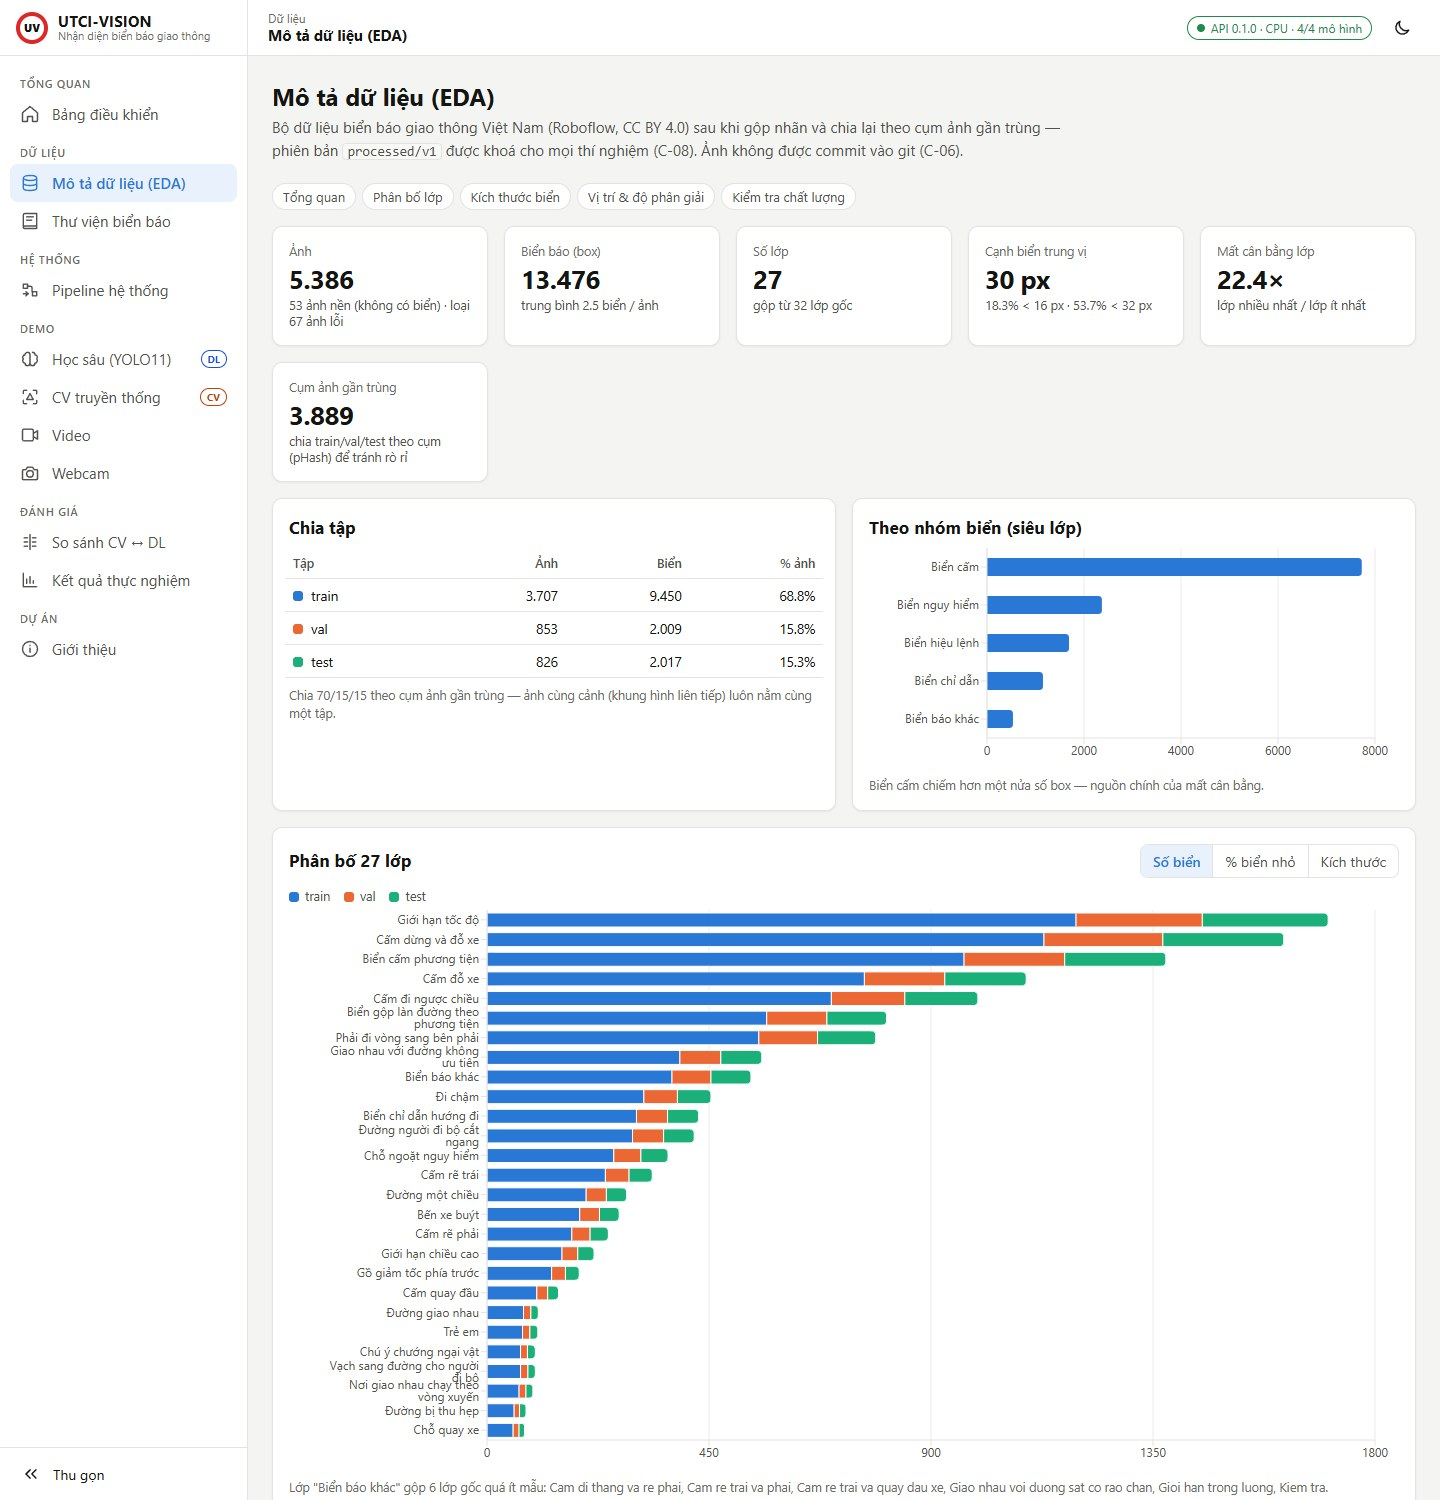
\includegraphics[width=.8\textwidth]{figures/web_eda.jpg}
\caption{Trang Mô tả dữ liệu của ứng dụng web}
\label{fig:web_eda}
\end{figure}

\begin{figure}[H]
\centering
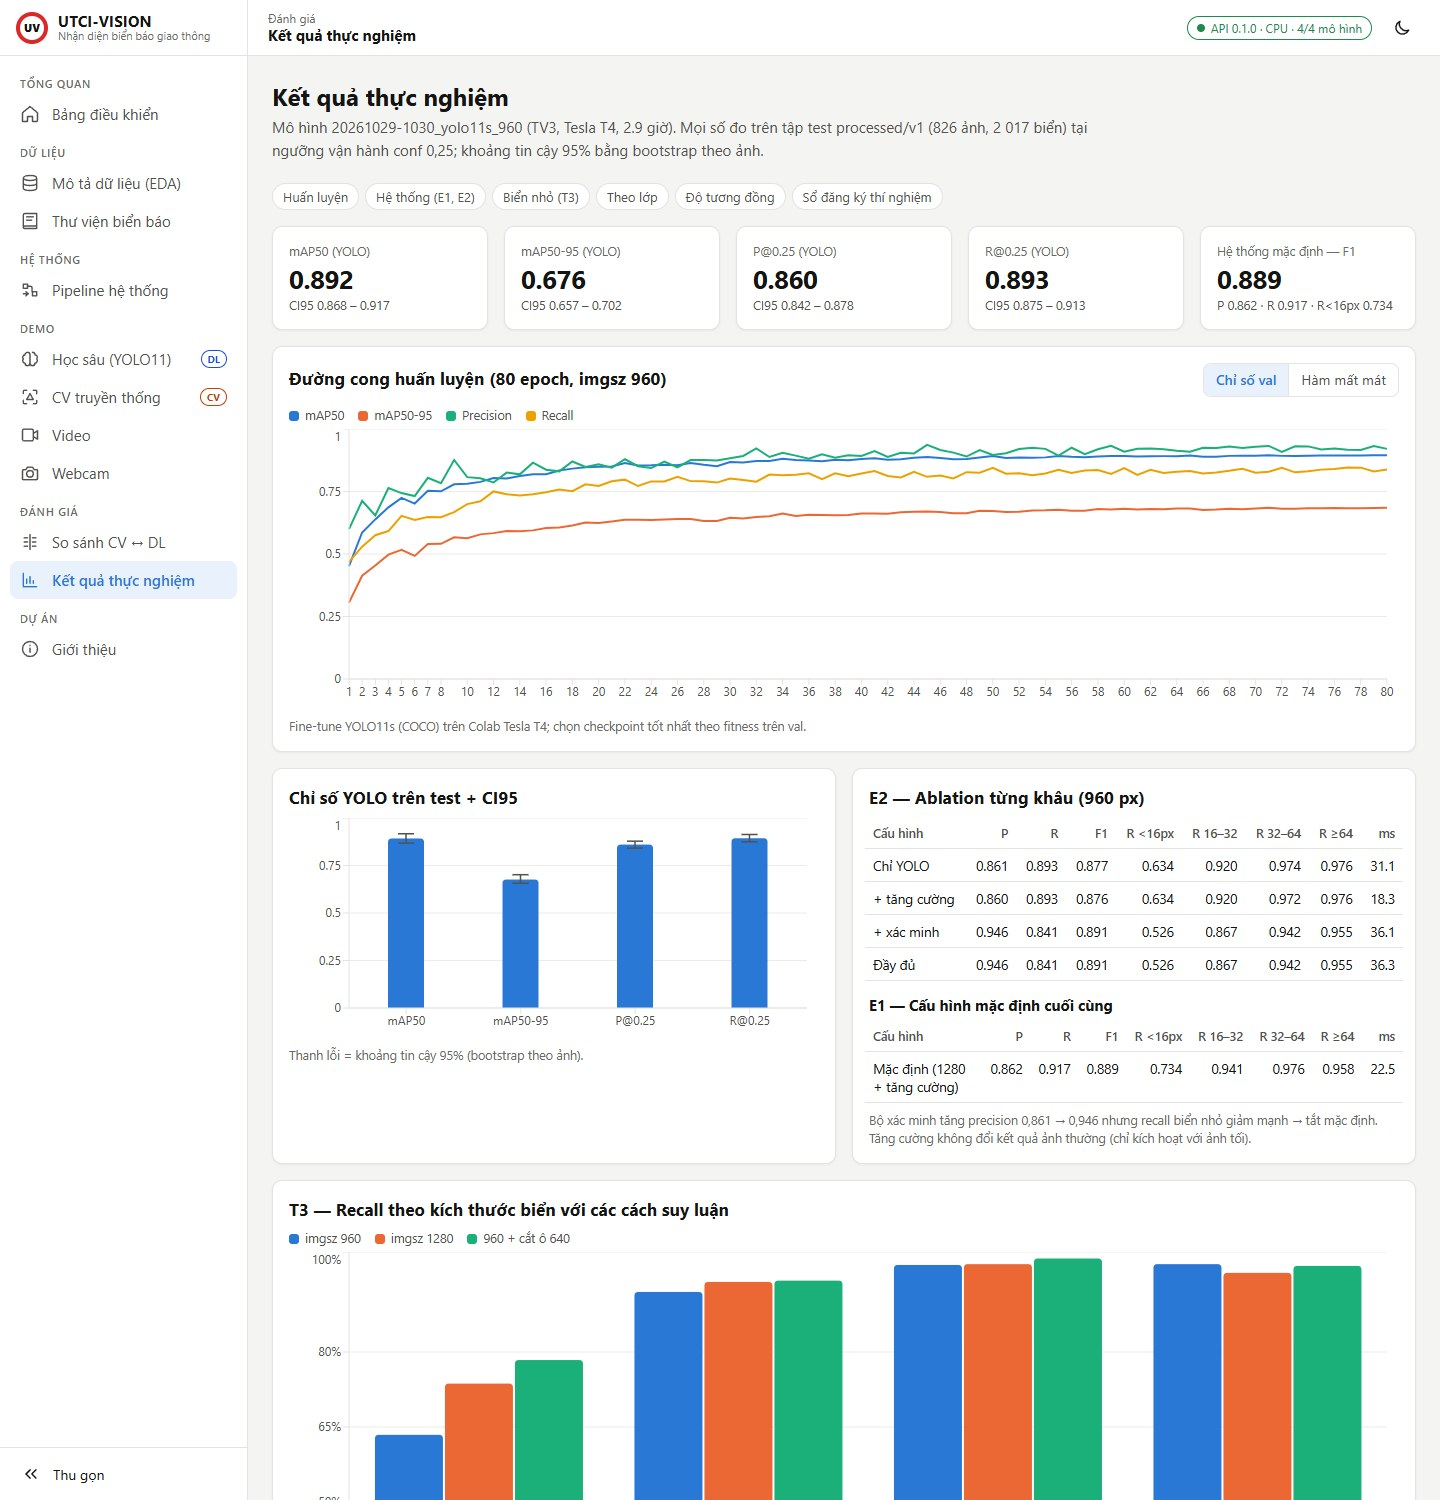
\includegraphics[width=.8\textwidth]{figures/web_results.jpg}
\caption{Trang Kết quả thực nghiệm của ứng dụng web}
\label{fig:web_results}
\end{figure}


\end{document}
